% IMPORT SETTINGS
\documentclass[12pt,a4paper,twoside]{thesisreport}

% Number of people who responded to the survey
\newcommand{\participantCount}{55}


% BASIC SETTINGS
\usepackage{moreverb}								% List settings
\usepackage{textcomp}								% Fonts, symbols etc.
\usepackage{lmodern}								% Latin modern font
\usepackage{helvet}									% Enables font switching
\usepackage[T1]{fontenc}							% Output settings
\usepackage[english]{babel}							% Language settings
\usepackage[utf8]{inputenc}							% Input settings
\usepackage{amsmath}								% Mathematical expressions (American mathematical society)
\usepackage{amssymb}								% Mathematical symbols (American mathematical society)
\usepackage{graphicx}								% Figures
\usepackage{subfig}									% Enables subfigures
\numberwithin{equation}{chapter}					% Numbering order for equations
\numberwithin{figure}{chapter}						% Numbering order for figures
\numberwithin{table}{chapter}						% Numbering order for tables
\usepackage{listings}								% Enables source code listings
\usepackage{chemfig}								% Chemical structures
\usepackage[top=3cm, bottom=3cm,
			inner=3cm, outer=3cm]{geometry}			% Page margin lengths			
\usepackage{eso-pic}								% Create cover page background
% \usepackage{todonotes} % To add in-document comments
\usepackage{enumitem} % For list customisation, used in appendix 1

\newcommand{\backgroundpic}[3]{
	\put(#1,#2){
	\parbox[b][\paperheight]{\paperwidth}{
	\centering
	\includegraphics[width=\paperwidth,height=\paperheight,keepaspectratio]{#3}}}}
\usepackage{float} 									% Enables object position enforcement using [H]

% DEFINE THESIS TYPE
\def\ThesisType{M} % M - master, B - bachelor

% COLOR FOR HEADERS
\definecolor{headerBrown}{RGB}{144,102,78}
\if\ThesisType B
\definecolor{thesisHeaderColor}{RGB}{126,180,56} % Green
\fi
\if\ThesisType M
\definecolor{thesisHeaderColor}{cmyk}{0.14,0,0,0.65} % Gray
\fi


% Caption settings (aligned left with bold name)
\usepackage[labelfont=bf, textfont=normal,
			justification=justified,
			singlelinecheck=false]{caption} 		

		  	
% Activate clickable links in table of contents  	
\usepackage{hyperref}
\hypersetup{
    colorlinks,
    citecolor  = blue, % If you want citation links to be blue as well
    filecolor  = blue, % Color for URLs which open local files
    linkcolor  = black, % Color for internal links (sections, pages, etc.)
    urlcolor   = blue,  % Color for linked URLs
    pdfpagemode=FullScreen
}

% Define the number of section levels to be included in the t.o.c. and numbered	(3 is default)	
\setcounter{tocdepth}{5}							
\setcounter{secnumdepth}{5}	


% Chapter title settings
\usepackage{titlesec}		
\titleformat{\chapter}[display]
  {\Huge\bfseries\filcenter}
  {{\fontsize{50pt}{1em}\vspace{-4.2ex}\selectfont \textnormal{\thechapter}}}{1ex}{}[]


% Header and footer settings (Select TWOSIDE or ONESIDE layout below)
\usepackage{fancyhdr}								
\pagestyle{fancy}  
\renewcommand{\chaptermark}[1]{\markboth{\thechapter.\space#1}{}} 


% Select one-sided (1) or two-sided (2) page numbering
\def\layout{2}	% Choose 1 for one-sided or 2 for two-sided layout
% Conditional expression based on the layout choice
\ifnum\layout=2	% Two-sided
    \fancyhf{}			 						
	\fancyhead[LE,RO]{\nouppercase{ \leftmark}}
	\fancyfoot[LE,RO]{\thepage}
	\fancypagestyle{plain}{			% Redefine the plain page style
	\fancyhf{}
	\renewcommand{\headrulewidth}{0pt} 		
	\fancyfoot[LE,RO]{\thepage}}	
\else			% One-sided  	
  	\fancyhf{}					
	\fancyhead[C]{\nouppercase{ \leftmark}}
	\fancyfoot[C]{\thepage}
\fi


\setlength{\marginparwidth}{2.5cm} 


% Supress warning from Texmaker about headheight
\setlength{\headheight}{15pt}		


% Tag command (invisible)
\newcommand{\tagtemp}{\textcolor{white}{, template by Kyriaki Antoniadou-Plytaria}}

% Allow a table to split
\usepackage{longtable}

% ALL VARIABLES USED IN THE THESIS: 
\newcommand{\authorp}{Prasannjeet Singh}
\newcommand{\authorm}{Muhammad Manssor Azeem}
\newcommand{\authort}{Mohsen Tafti}
\newcommand{\university}{Blekinge Institute Of Technology}
\newcommand{\dept}{Department of Industrial Economics}
\newcommand{\maintitle}{Evaluating the Impact of COVID-19 on Supply Chain Resilience for Perishable Goods: A Mixed-Methods Approach to Challenges and Strategic Responses}
\newcommand{\address}{Karlskrona, Sweden}
\newcommand{\site}{www.bth.se}
\newcommand{\subject}{IY2594 V24 Master's Thesis}
\newcommand{\supervisor}{Viroj Jienwatcharamongkhol}
\newcommand{\examiner}{Johanna Börrefors}
% 

% References %
\usepackage{csquotes} % Add this line to your preamble

\usepackage[
backend=biber,
style=apa, % Reference style (APA)
% sorting=none, % Sort references by first occurrence
uniquename=init,
giveninits
]{biblatex}
\addbibresource{references.bib}
\addbibresource{mendeley.bib}

% Automatically add "no date" for references without a given year
\newcommand{\mkbibnodate}{\GetTranslation{no-date}}
\AtEveryCitekey{\iffieldundef{labelyear}{\restorefield{labelyear}{\mkbibnodate}\restorefield{year}{\mkbibnodate}}{}}

\AtEveryBibitem{\iffieldundef{labelyear}{\restorefield{labelyear}{\mkbibnodate}\restorefield{year}{\mkbibnodate}}{}}


\usepackage{tabularx} % For tables auto fitting 

% Enable To-do notes
\usepackage[textsize=tiny]{todonotes}   % Include the option "disable" to hide all notes

% So that image captions are in the center
% \usepackage[justification=centering]{caption}
\usepackage{caption}

% To add colored box
\usepackage{tcolorbox}  
\usepackage{booktabs}


% Paragrap spacing
% \usepackage[parfill]{parskip}
% \setlength{\parindent}{0em} % Indent the first line of each paragraph
% \setlength{\parskip}{1 em}
% \setlength{\parskip}{10pt plus 1pt minus 1pt}

% \parskip = \baselineskip
% \multiply \parskip by 5
% \parskip = 2\baselineskip % no shrink and no stretch
% \setlength{\parskip}{\baselineskip}%
% \setlength\parskip{6pt}

% \usepackage[parfill]{parskip}
\setlength{\parindent}{0em}
% \setlength{\parskip}{2em}
% \setlength{\parskip}{1em}
% \parskip = \baselineskip


\begin{document} 

% If you write a bachelor thesis, change \def\ThesisType{M} to \def\ThesisType{B} in Settings.tex

% COVER PAGE, TITLE PAGE AND IMPRINT PAGE
\pagenumbering{roman}			% Roman numbering (starting with i (one)) until first main chapter
\ifx\ThesisType\undefined
Undefined Thesis type in settings.tex
\else
  \if\ThesisType M
    \else
    \if\ThesisType B
    \else
    Define \textbackslash ThesisType as M for master's thesis or B for bachelor thesis in settings.tex
    \fi
  \fi
\fi

% COVER PAGE
\begin{titlepage}
\newgeometry{top=3cm, bottom=1cm,
			left=2.25 cm, right=2.25cm}	% Temporarily change margins		
			
%Header Front Page
\ifx\ThesisType\undefined
\else
    \if\ThesisType M
    \vtop{
        \null\vspace{-25mm}
        \centerline{
\includegraphics[width=1.18\textwidth]{figure/auxiliary/GrayHeaderPattern.jpg}}
        \vspace{-2.3cm}
        \hbox{\hspace{0mm}
\includegraphics[height=18mm]{figure/auxiliary/logo_swe.png}}
        \centerline{\textcolor{headerBrown}{\rule{1.18\textwidth}{4pt}}}
        \vspace{\paperheight}\vspace{-85mm}
        \centerline{\textcolor{thesisHeaderColor}{\rule{1.1\textwidth}{0.8pt}}} % Rule after Department
        \vspace{-\paperheight}\vspace{85mm}
    }
    \fi
    \if\ThesisType B
    \vtop{
        \null\vspace{-25mm}
        \centerline{
\includegraphics[width=1.18\textwidth,height=80pt]{figure/auxiliary/GreenHeaderPattern.jpg}}
        \vspace{-2.3cm}
        \hbox{\hspace{0mm}\includegraphics[height=18mm]{figure/auxiliary/long_swe.png}}
        \centerline{\textcolor{headerBrown}{\rule{1.18\textwidth}{4pt}}}
        \vspace{\paperheight}\vspace{-85mm}
        \centerline{\textcolor{thesisHeaderColor}{\rule{1.1\textwidth}{0.8pt}}} % Rule after Department
        \vspace{-\paperheight}\vspace{85mm}
    }
    \fi
\fi

% Cover picture (replace with your own or delete)		
\begin{figure}[H]
\centering
\vspace{1cm}	% Adjust vertical spacing here
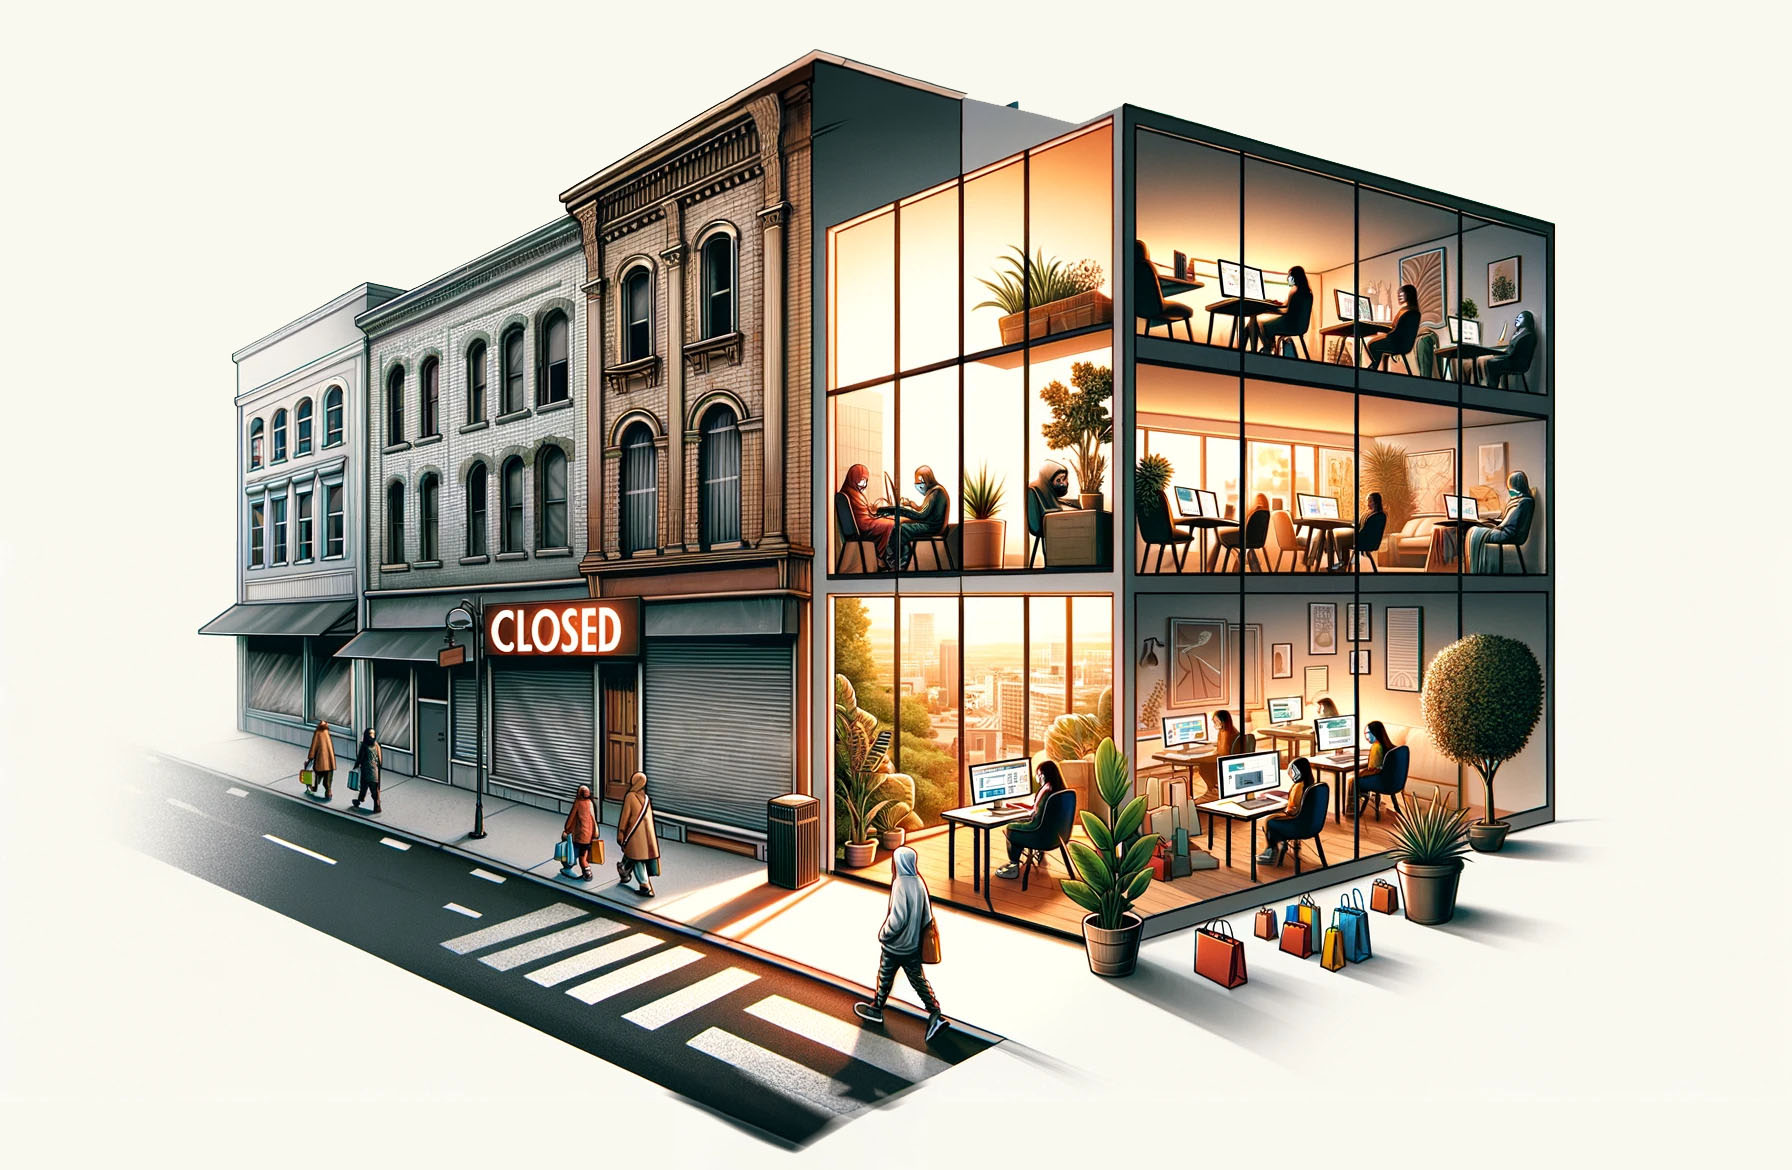
\includegraphics[width=0.9\linewidth]{figure/art2.jpg}
\end{figure}

% Cover text
\mbox{}
\vfill
\renewcommand{\familydefault}{\sfdefault} \normalfont % Set cover page font
\textbf{{\Huge 	\maintitle 	\\[0.2cm] }} 	\\[0.5cm]

% {\small \maintitle \\[0.2cm]}
    
% {\Large A Subtitle that can be Very Much Longer if Necessary}\\[0.5cm]
% Master's thesis in Master Programme Name \setlength{\parskip}{1cm}

\noindent
{\Large \authorm \\[0.18cm]
\authorp \\[0.1cm]
\authort
} \setlength{\parskip}{1.5cm}

\noindent
\textcolor{thesisHeaderColor}{\small\textbf{\textsc{\dept}}}
\setlength{\parskip}{1mm}

\textsc{\university} \\
{\small \address \the\year \\
\href{\site}{\site}}\vspace{1.7cm}

\renewcommand{\familydefault}{\rmdefault} \normalfont % Reset standard font
\end{titlepage}
% % BACK OF COVER PAGE (BLANK PAGE)
\newpage
\restoregeometry
\thispagestyle{empty}
\mbox{}


% TITLE PAGE
\newpage
\thispagestyle{empty}
\begin{center}
	\textsc{\large \subject \the\year}\\[4cm]
	\textbf{\Large \maintitle} \\[1cm]
	% {\large A Subtitle that can be Very Much Longer if Necessary}\\[1cm]
	{\large \authorm} \\[0.1cm]
        {\large \authorp} \\[0.1cm]
        {\large \authort}
	
	\vfill	
	% Logotype on titlepage	
	\begin{figure}[H]
	\centering
	% Remove this figure to remove the titlepage logotype
	\if\ThesisType M
    
\includegraphics[width=0.2\pdfpagewidth]{figure/auxiliary/logo_circle.png} \\
    \fi
    \if\ThesisType B
    
\includegraphics[width=0.2\pdfpagewidth]{figure/auxiliary/logo_circle.png} \\
    \fi

	\end{figure}	\vspace{5mm}	
	
	\dept \\
	% \emph{Division of Division name}\\
	% Name of research group (if applicable)\\
	\textsc{\university} \\
	\address \  \the\year \\
\end{center}

% IMPRINT PAGE (BACK OF TITLE PAGE)
\newpage
\thispagestyle{plain}
\vspace*{3.5cm}
\maintitle \\
% A Subtitle that can be Very Much Longer if Necessary\\
\\[0.1cm]
\authorm \\
\authorp \\
\authort
\setlength{\parskip}{1cm}

% \copyright ~ NAME FAMILYNAME, \the\year. \setlength{\parskip}{1cm}

Supervisor: \supervisor \\
Examiner: \examiner \setlength{\parskip}{1cm}

\subject \\	
\dept \\
% Division of Division name\\
% Name of research group (if applicable)\\
\university \\
\address \\
% Telephone +46 31 772 1000 
\setlength{\parskip}{0.5cm}


% \vfill
\vspace*{5.5cm}
% Caption for cover page figure if used, possibly with reference to further information in the report
Cover - \textbf{Contrast in Commerce:} A Generative Image of Closed Shops and Bustling Online Markets. \setlength{\parskip}{0.5cm}

Typeset in \LaTeX \tagtemp\\
% Printed by XXX \\
\address \ \the\year \\
\today

\newpage

% ABSTRACT
% \newpage
\thispagestyle{plain}			% Supress header 
% \setlength{\parskip}{0pt plus 1.0pt}
\section*{Abstract}

The COVID-19 pandemic has profoundly impacted global supply chains, particularly in the sectors of e-commerce and perishable goods. This study investigates the significant disruptions experienced by suppliers of perishable goods and the subsequent strategic adaptations made to enhance supply chain resilience. The pandemic catalyzed a rapid transformation in consumer behavior, leading to a surge in online shopping and an increased reliance on digital platforms. This shift exacerbated supply chain vulnerabilities, particularly during the initial stages of the pandemic, where inventory shortages, transportation delays, and logistical bottlenecks were prevalent. The challenges were further intensified by external events such as the Suez Canal blockage, which underscored the fragility of global supply chains and the necessity for rapid adjustments in inventory management strategies.

The study also highlights the contrasting effects of the pandemic across different regions, with significant disruptions observed in both the U.S. and Asia. In the U.S., e-commerce businesses faced additional fulfillment challenges due to lockdowns and restrictions, particularly in the distribution of non-essential products. In Asia, the pandemic led to factory shutdowns, causing delays in manufacturing and a shortage of critical items, particularly in the healthcare, automotive, and food industries. These disruptions were compounded by restrictions on movement, leading to delays and cancellations of shipments and further bottlenecks in cross-border trade.

In response to these challenges, suppliers of perishable goods have implemented a range of strategies to enhance supply chain resilience. These include local warehousing, diversification of suppliers, and increased collaboration across the supply chain. The adoption of technology for real-time data sharing and the creation of crisis management teams are indicative of a proactive approach to managing future disruptions. The evidence suggests a strategic shift towards more resilient and flexible supply chains, with a focus on improving robustness and preparedness in anticipation of future crises.

With a mixed-method approach of questionnaires and interviews we discuss the significant disruptions in the supply chain of perishable goods due to COVID-19 and provide methods and strategies the suppliers and supermarkets have used to minimize the impact on the supply chain and increase the resilience of it to future similar events. The study concludes that the pandemic has led to substantial changes in e-commerce strategies and logistics operations, emphasizing the need for continued adaptation to the evolving market and consumer needs in the post-pandemic era.











% KEYWORDS (MAXIMUM 10 WORDS)
\vfill
\begin{flushleft}
Keywords: Supply Chain, Disruption, Resilient Supply Chain, Digitalization, Long-term Strategy.
\end{flushleft}
\break
% References: \parencite{fryer_2020_understanding, zhao_2018_research, Musella2023TheFragilities}

% \newpage				% Create empty back of side
% \thispagestyle{empty}
% \mbox{}

% ACKNOWLEDGEMENTS
% \newpage
\thispagestyle{plain}			% Supress header
\section*{Acknowledgements}


\vspace{1.5cm}
\hfill
Name

% \newpage				% Create empty back of side
\thispagestyle{empty}
\mbox{}

% Acronyms
% \newpage
\addcontentsline{toc}{chapter}{List of Acronyms}
\input{include/frontmatter/Acronyms}

% Nomenclature
% \newpage
% \addcontentsline{toc}{chapter}{Nomenclature}
% \input{include/frontmatter/Nomenclature}

% TABLE OF CONTENTS
% \newpage
\setlength{\parskip}{0em}
\tableofcontents

% OTHER FRONTMATTER
% List of figures (add to table of contents)
% \cleardoublepage
\addcontentsline{toc}{chapter}{\listfigurename} 
\listoffigures
% List of tables (add to table of contents)
% \cleardoublepage
\addcontentsline{toc}{chapter}{\listtablename}  
\listoftables


% START OF MAIN DOCUMENT
% \cleardoublepage
\setcounter{page}{1}
\pagenumbering{arabic}

% INTRODUCTION
\parskip = 8pt plus 2pt minus 2pt
\setlength{\parindent}{5em}
\chapter{Background}

The novel coronavirus (COVID-19) pandemic has emerged as one of the most significant global health crises of the 21st century, affecting nations across the world irrespective of economic status or healthcare capacity. Originating in Wuhan, China, in late 2019, the virus has demonstrated the profound interconnectedness of modern societies, exposing vulnerabilities in public health systems, economies, and the fabric of global cooperation \parencite{Verma2021AReturns, Shrestha2020TheGlobalization, LegeseFeyisa2020TheReview, MaitalEllaBarzani2020EResearch}.  

\section{The Unprecedented Impact of COVID-19}

COVID-19 has underscored the fragility of the global economy, causing widespread economic disruptions, from the decimation of industries such as travel and tourism to unprecedented levels of unemployment and poverty \parencite{Verma2021AReturns, LegeseFeyisa2020TheReview}. The pandemic has catalyzed a deep recession, with the World Bank and the International Monetary Fund predicting a contraction in global GDP unparalleled in recent history \parencite{Verma2021AReturns, Shrestha2020TheGlobalization, LegeseFeyisa2020TheReview, MaitalEllaBarzani2020EResearch}. The abrupt halt in economic activity has led to a significant decline in stock markets worldwide, reflecting investor uncertainty and fear \parencite{Verma2021AReturns}.

The response to the pandemic has varied globally, with nations implementing lock-downs, social distancing measures, and mass testing in attempts to curb the spread of the virus. These measures, while necessary for public health, have further strained economies, leading to a comprehensive debate on balancing health outcomes with economic sustainability \parencite{Shrestha2020TheGlobalization, LegeseFeyisa2020TheReview}.

\section{Learning from History for Future Preparedness}

Historically, pandemics have been recurrent challenges for humanity, with the 1918 Spanish Flu being a notable reference point for COVID-19 due to its widespread impact and high mortality rate. Similar to past pandemics, COVID-19 has highlighted the critical need for robust healthcare systems, rapid response mechanisms, and global cooperation in surveillance and vaccine development \parencite{Shrestha2020TheGlobalization, MaitalEllaBarzani2020EResearch}. The pandemic has also emphasized the importance of non-pharmaceutical interventions, such as social distancing and hygiene practices, which have become the first line of defense in the absence of a vaccine \parencite{LegeseFeyisa2020TheReview, MaitalEllaBarzani2020EResearch}.

\section{The Role of Technology and Innovation}

The COVID-19 crisis has accelerated the adoption of technology and innovation across various sectors. Telemedicine, remote work, and e-learning have become the new norm, suggesting a long-term transformation in how societies operate. This shift presents an opportunity to re-imagine future responses to pandemics, with a focus on digital infrastructure, data analytics for disease surveillance, and a more agile healthcare delivery model \parencite{Shrestha2020TheGlobalization, MaitalEllaBarzani2020EResearch}.

\section{A Call for Global Solidarity and Preparedness}

The COVID-19 pandemic has served as a stark reminder of the global community's interconnectedness and the collective vulnerability to emerging pathogens. It underscores the necessity for a unified global response strategy, investments in healthcare infrastructure, and the importance of preparedness plans that are adaptable and scalable in the face of future pandemics. The lessons learned from COVID-19 should guide international policy, research, and cooperation, ensuring that the world is better equipped to face similar challenges in the future \parencite{Verma2021AReturns, Shrestha2020TheGlobalization, LegeseFeyisa2020TheReview, MaitalEllaBarzani2020EResearch}.

\section{Supply Chain Management and the Needs for Constant Improvement}

Supply chain management is a critical aspect of any industry, with the food industry being particularly sensitive due to the nature of its products and the importance of maintaining quality and safety. In today’s rapidly evolving global market, various vulnerabilities within the supply chain can have significant impacts on both businesses and consumers.

One of the pressing concerns is identifying specific vulnerabilities within supply chains. For instance, what happens if we encountered health-related problems in the food industry due to supply chain issues? Understanding these vulnerabilities is crucial for developing robust strategies to mitigate risks. If and when we encounter a real-world example of a health-related problem in the food industry. How was it caused, and what were the outcomes? These situations highlight the importance of having complete end-to-end visibility in the supply chain. However, achieving such transparency comes with its own set of challenges\parencite{Wagner2006AnVulnerability, Elleuch2016ResilienceReview}.

To address these vulnerabilities, avoiding over-reliance on single sources is a key strategy in mitigating risk. What are the strategies we can use to diversify our supply sources effectively? Furthermore, how adaptable and flexible the current supply chain is in responding to fluctuations in demand or supply\parencite{Yin2022SupplyFsQCA, Wang2024TheCOVID-19, Lin2021TheManufacturers}.

Balancing cost efficiency with other factors like safety and quality is another challenge, especially in the context of global operations such as temperature-controlled transport. What is the optimal inventory strategy to achieve this balance? How does this strategy apply on a global scale?

Collaboration with suppliers and partners is essential for improving transparency, trust, and joint risk management. During unprecedented events like pandemics, what kinds of collaboration have proven effective? Similarly, how can technologies like AI and IoT help solve tracking and traceability challenges, thereby enhancing the overall supply chain\parencite{Wang2024TheCOVID-19, Simatupang2002TheChain, Singh2023Post-COVIDVaccination, Ramanathan2014SupplyPartnerships, Chen2017SupplyAgenda}?

With increasing scrutiny of regulating and governing bodies such as EU-Parliament on environmental impacts and green supply chain \parencite{Amann2014DrivingUnion, Moazzem2022EnvironmentalProducts}, ensuring compliance with global regulations while maintaining a commitment to sustainability is another critical consideration. What strategies can be employed to reduce waste and ensure the proper use of resources? Moreover, do you have comprehensive crisis management plans that address supply chain disruptions, and how were these plans tested during the COVID-19 pandemic?

Rapid recovery from supply chain disruptions requires well-thought-out strategies. Can you provide examples of successful recovery strategies? During the COVID-19 pandemic, what were the most significant challenges faced, especially concerning perishable goods? Looking ahead, what are the main concerns regarding the potential impact of future pandemics on perishable goods, and what measures can the industry take to improve resilience\parencite{Chowdhury2021COVID-19Review, Paul2021SupplyPandemic, Ivanov2017LiteratureChain, Chen2019BuildingIndustry}? 

In conclusion, the resilience and adaptability of the supply chain are of paramount importance, especially in the face of unforeseen challenges. By exploring these questions, we can better understand the intricacies of supply chain management and develop strategies to ensure its robustness in the future.

% The COVID-19 pandemic has brought about unprecedented changes in consumer behavior and retail dynamics, presenting a compelling need for in-depth analysis. This research is motivated by several key factors:

% \begin{itemize}
%     \item \textbf{Transformation in Consumer Behavior}: The pandemic has radically altered how consumers shop, work, and live. New personal circumstances, such as changes in income and leisure time, have significantly influenced consumer attitudes and behaviors. Consumers have become more conscious of environmental, health, and cost factors, leading to a preference for locally-sourced products and neighborhood stores. Notably, there has been a significant rise in digital commerce, especially among new or low-frequency users, which is expected to continue post-pandemic \parencite{standish_2020_covid19}.

%     \item \textbf{Lasting Impact on Retail and E-Commerce}: The shifts in consumer behavior are not just transient reactions to the pandemic but are likely to have long-term implications for the retail industry. Companies have an opportunity to help shape the 'next normal' as many of the longer-term changes in consumer behavior are still forming. This presents a unique challenge and opportunity for retailers and consumer packaged goods companies to adapt and evolve in response to these changes \parencite{fabius_2020_how}.

%     \item \textbf{Need for Strategic Adaptation}: Understanding these behavioral shifts is crucial for businesses to develop effective strategies for the post-pandemic market. This includes rethinking supply chain management, marketing strategies, and logistics operations to align with the evolving consumer preferences and shopping habits.

%     \item \textbf{Resilience and Response to Future Uncertainties}: Analyzing how the pandemic has transformed consumer behavior and retail dynamics can provide insights into how businesses and consumers respond to uncertainties. This knowledge can be instrumental in preparing for future crises, ensuring more resilient and adaptable business models.
    
% \end{itemize}

% this research is vital for comprehending the extensive and potentially lasting changes brought about by the COVID-19 pandemic in the realm of consumer behavior and retail. It offers valuable insights for businesses to adapt to the evolving market and consumer needs in the post-pandemic era, and to prepare for future challenges. This is a citation \parencite[p.~12]{guo2022has}. \textcite[p.~12]{guo2022has} has proposed something. In Figure \ref{fig:covid_art2} there is covid art.

% \begin{figure}[htbp] % Positioning option: h=here, t=top, b=bottom, p=page of floats
%   \centering % Centers the image
%   \fbox{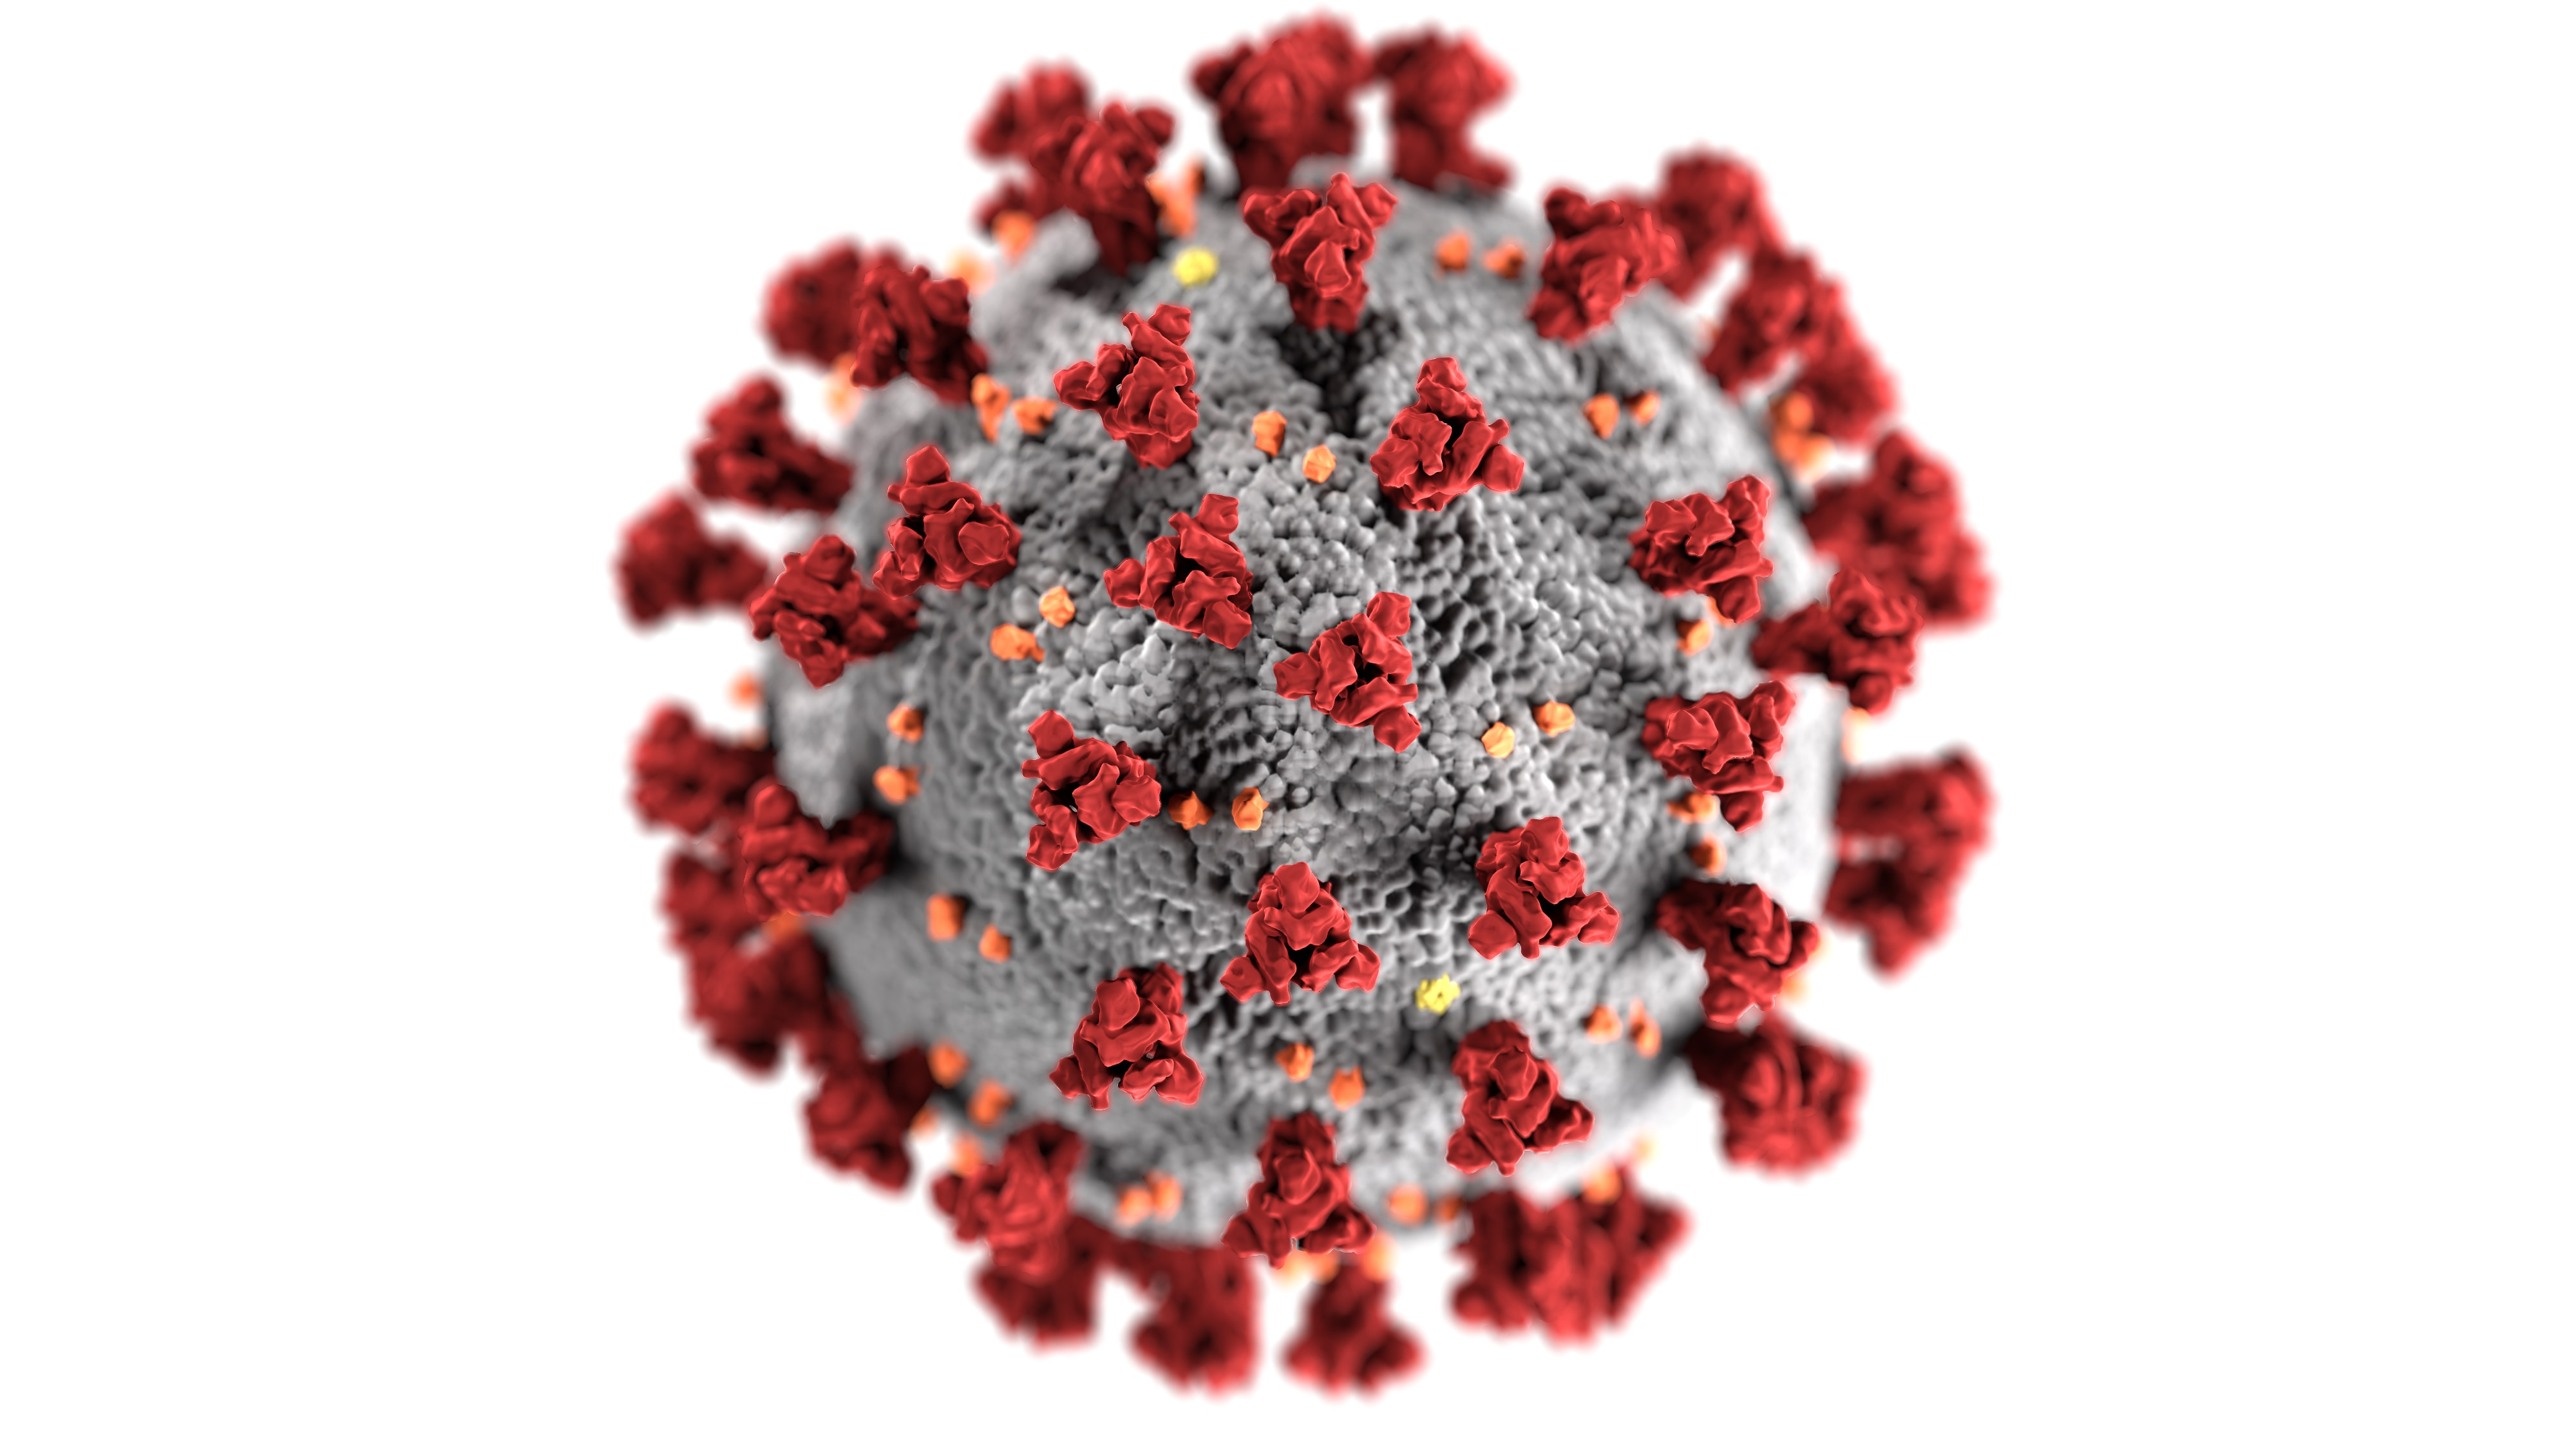
\includegraphics[width=0.8\textwidth]{figure/covid_art.jpg}}
%   \caption{Sample COVID art.}
%   \label{fig:covid_art} 
% \end{figure}

% \begin{figure}[htbp] % Positioning option: h=here, t=top, b=bottom, p=page of floats
%   \centering % Centers the image
%   \fbox{
\includegraphics[width=0.8\textwidth]{figure/art.jpg}}
%   \caption{Some caption.}
%   \label{fig:covid_art2} 
% \end{figure}

% \parencite{guo2022has}
% \textcite{guo2022has}
% \textcite[p.~12]{guo2022has}

% \begin{itemize}
%     \item Transformation in Consumer Behavior: The pandemic has radically altered how consumers shop, work, and live. New personal circumstances, such as changes in income and leisure time, have significantly influenced consumer attitudes and behaviors. Consumers have become more conscious of environmental, health, and cost factors, leading to a preference for locally-sourced products and neighborhood stores. Notably, there has been a significant rise in digital commerce, especially among new or low-frequency users, which is expected to continue post-pandemic (Standish, 2020).
    
%     \item Lasting Impact on Retail and E-Commerce: The shifts in consumer behavior are not just transient reactions to the pandemic but are likely to have long-term implications for the retail industry. Companies have an opportunity to help shape the 'next normal' as many of the longer-term changes in consumer behavior are still forming. This presents a unique challenge and opportunity for retailers and consumer packaged goods companies to adapt and evolve in response to these changes (Fabius, 2020).
    
%     \item Need for Strategic Adaptation: Understanding these behavioral shifts is crucial for businesses to develop effective strategies for the post-pandemic market. This includes rethinking supply chain management, marketing strategies, and logistics operations to align with the evolving consumer preferences and shopping habits.
% \end{itemize}


% THEORY
\chapter{Literature Review}
\label{chap:literature}

\section{Overview of the Pandemic's Impact on Global Supply Chains and E-commerce}

The COVID-19 pandemic has ushered in an era of unprecedented challenges and transformations across the globe, significantly impacting global supply chains and e-commerce. This section delves into the multifaceted effects of the pandemic, drawing on insights from some pivotal studies that explore the resilience of supply chains, and the accelerated adoption of e-commerce.

The pandemic also significantly disrupted global supply chains, exposing vulnerabilities and prompting a reevaluation of supply chain resilience across various sectors. The surge in global e-commerce sales, which reached \$$4.9$ trillion in 2019 — an 11\% increase from the previous year—highlighted the growing demand for robust and flexible supply chains, particularly in regions like the United States, Japan, and China \parencite{KofiMensah2021Cross-BorderReview}. As physical stores closed and social distancing measures were implemented, the reliance on e-commerce intensified, pressuring supply chains to adapt quickly to meet the sudden shift in consumer demand, especially in countries like China, India, and Vietnam \parencite{KofiMensah2021Cross-BorderReview}. In Canada, the pandemic's impact on supply chains was particularly evident in the grocery sector, where the increased demand for online food procurement tested the resilience of existing supply networks. Before the pandemic, 46.4\% of consumers had not ordered food online; however, the need for contactless shopping due to health concerns caused a dramatic shift, compelling supply chains to adjust to the new demands of online food ordering across multiple generations \parencite{Charlebois2021SupplyStudy}. This widespread shift stressed the critical importance of strengthening supply chains to ensure they can withstand future disruptions and continue to meet consumer needs effectively. Furthermore, significant drop was observed in the volume of containers transported from China to the U.S. and the indefinite closure of factories and warehouses \parencite{Miljenovic2022PandemicsPandemic}. Despite these challenges, the pandemic highlighted the advantages of the drop shipping model, which allows for direct delivery from the manufacturer to the retailer or customer, showcasing its adaptability and efficiency in a crisis \parencite{Miljenovic2022PandemicsPandemic}. This model facilitated global delivery solutions, emphasizing the need for businesses to adopt more flexible and resilient supply chain strategies. The adoption of artificial intelligence (AI) and other technological advancements played a crucial role in combating the pandemic's challenges, including monitoring infected individuals and ensuring the delivery of food and medication \parencite{KofiMensah2021Cross-BorderReview}. However, the increase in online sales also raised sustainability concerns, particularly regarding increased plastic pollution and the need for sustainable practices in the e-commerce era \parencite{Charlebois2021SupplyStudy}. Additionally, the pandemic has undeniably reshaped the landscape of global supply chains and e-commerce, accelerating digital transformation and highlighting the need for resilience and adaptability in the face of global disruptions. The insights from \textcite{Charlebois2021SupplyStudy, Miljenovic2022PandemicsPandemic, Din2022ThePurchasing, KofiMensah2021Cross-BorderReview} provide a comprehensive understanding of the pandemic's impact, offering valuable lessons for businesses, policymakers, and consumers as they navigate the post-pandemic world. The transition towards e-commerce, the challenges faced by supply chains, and the opportunities for innovation and sustainability are critical areas for future research and strategic planning.

\section{Resilient Supply Chains}

The COVID-19 pandemic has underlined the critical importance of resilient supply chains in maintaining the flow of goods and services during global disruptions. This section explores the concept of supply chain resilience, pre-pandemic vulnerabilities, and strategies for developing resilient supply chains, drawing on insights from prominent studies. Supply chain resilience refers to the ability of a supply chain to anticipate, prepare for, respond to, and recover from unexpected disruptions. Resilience involves not just surviving disruptions but also thriving in the face of them by adapting and transforming supply chain operations \parencite{Mishra2024RedefiningFactors, Michel2023DimensionsPandemic, Cherrafi2022DigitalEra}. The COVID-19 pandemic has highlighted the need for resilience in the face of both internal and external systemic threats, including epidemics, pandemics, and other disruptions like natural disasters or terrorist attacks \parencite{Michel2023DimensionsPandemic}. The pandemic revealed several pre-existing vulnerabilities in global supply chains, including over-reliance on single sources of supply, lack of visibility and agility, and insufficient collaboration among supply chain partners. Over 94\% of Fortune 1,000 companies experienced disruptions due to the pandemic, exposing the fragility of global supply chains to high uncertainty, long-term disruptions, and the ripple effect propagation \parencite{Cherrafi2022DigitalEra}. These vulnerabilities spotlight the necessity for supply chains to be more than just efficient; they must also be resilient.

\subsection{Strategies for Developing Resilient Supply Chains}

\begin{itemize}
    \item \textbf{Diversification of Supply Sources: }Diversification of supply sources mitigates risks associated with supplier concentration in specific regions, which became evident when localized outbreaks and restrictions led to significant disruptions \parencite{Cherrafi2022DigitalEra}. The pandemic has prompted a reevaluation of globalized supply chains, with a call for regionalization and diversification to reduce dependency on distant suppliers and mitigate risks \parencite{Cherrafi2022DigitalEra}.

    \item \textbf{Technology and Digital Transformation: }Digital technologies and circular economy practices have emerged as dynamic capabilities crucial for enhancing supply chain resilience and sustainability. These technologies can improve sensing, seizing, and transforming capabilities within supply chains, offering tools for better visibility, agility, and collaboration \parencite{Cherrafi2022DigitalEra}. The pandemic has accelerated the adoption of digital technologies, highlighting their role in ensuring supply chain continuity and resilience \parencite{Mishra2024RedefiningFactors, Cherrafi2022DigitalEra}.

    \item \textbf{Flexible Logistics and Distribution Models: }The agility of supply chains during the pandemic was crucial for managing volatility in demand and supply. Flexible logistics and distribution models, including on-demand warehousing and multi-modal transportation, have proven essential for adapting to rapidly changing conditions. Simplification of supply chains and innovative supply chain designs are suggested to manage and mitigate risks more effectively, making the system more predictable and manageable \parencite{Mishra2024RedefiningFactors}.

    \item \textbf{Collaboration and Information Sharing: }Collaboration among supply chain partners enhances visibility and responsiveness, which are vital for resilience. The importance of information systems (IS) in facilitating collaboration and ensuring effective communication across the supply chain was particularly highlighted during the pandemic. IS's involvement in all dimensions of resilience underscores its transversal importance in achieving a resilient supply chain \parencite{Michel2023DimensionsPandemic}.

    \item \textbf{Case Studies and Examples: }Real-world examples from the studies illustrate how organizations have navigated the challenges posed by the pandemic. Médecins Sans Frontières Logistique (MSF Log) demonstrated the ability to reorganize in response to crises through both reactive measures and proactive planning, emphasizing the balance of proactive and reactive measures required for effective resilience \parencite{Michel2023DimensionsPandemic}. The manufacturing industry, particularly the steel sector in India, provides empirical insights into the application of agile supply chain enablers, offering a comprehensive understanding of supply chain management in practical settings \parencite{Mishra2024RedefiningFactors}.

\end{itemize}


\section{Synthesis and Research Gaps}

The dynamics of supply chain resilience during the COVID-19 pandemic presents a critical area of study, particularly in the handling of perishable goods. This section synthesizes insights from \textcite{Li2010TheValue, RiveroGutierrez2020OmnichannelSector, Zhang2020IntegrationBOPS}, exploring how supply chains adapted to ensure the continuity and efficiency of food supply, and identifying gaps where further research is imperative.

\subsection{Adapting Supply Chain Strategies for Perishable Goods}

The onset of the pandemic required rapid adaptation of supply chain strategies to address the unique challenges of perishable goods distribution. This adaptation was crucial to maintain freshness and reduce wastage during periods of unpredictable demand and logistical disruptions. The feasibility of innovative distribution methods, such as "buy online and pick up in store" (BOPS), became increasingly relevant \parencite{Zhang2020IntegrationBOPS}. Although initially aligned with consumer convenience, the strategic value of BOPS in enhancing supply chain resilience through diversified distribution options has become evident. Such strategies reduce the dependency on traditional supply routes and help manage the perishable goods more efficiently.

In sectors where timely delivery is critical, the integration of advanced digital solutions has proven essential. For instance, in highly regulated sectors like healthcare, the adaptation of omnichannel approaches ensures operational resilience \parencite{RiveroGutierrez2020OmnichannelSector}. The application of similar strategies in the food sector, combining digital and physical distribution channels, could significantly enhance the responsiveness and flexibility of supply chains dealing with perishable items. However, the implementation of these adaptive strategies raises questions about optimal conditions and the scalability of such models. The study by \textcite{Zhang2020IntegrationBOPS} provides a mathematical model to explore these conditions, suggesting that the scale of implementation and the specific characteristics of supply chain networks significantly influence the success of adaptive strategies \parencite{Zhang2020IntegrationBOPS}. This highlights a clear research gap in understanding how scalable and flexible supply chain models can be effectively designed and implemented to cope with future disruptions.

\subsection{Identifying Research Gaps}

The studies reviewed thus far provide a foundational understanding of how supply chains have adapted during the COVID-19 pandemic, particularly in handling perishable goods. However, these insights reveal several areas where further investigation is crucial. There remains a significant gap in understanding the full impact of technological advancements on supply chain resilience. Emerging technologies such as artificial intelligence (AI) and blockchain have shown potential to revolutionize supply chain management by enhancing efficiency, transparency, and responsiveness. Detailed research is needed to evaluate how these technologies can be specifically leveraged to bolster the resilience of supply chains managing perishable goods. This is critical for ensuring that food supplies remain safe and efficient, minimizing waste and improving distribution even under disruptive conditions. Additionally, the adaptations and strategies developed for specific sectors during the pandemic, such as the implementation of advanced digital solutions in regulated environments like healthcare, suggest that similar strategies could be applied to the perishable goods sector. More focused studies are required to explore how these strategies can be tailored to meet the unique demands and challenges of different industries, ensuring that supply chains can withstand not only current disruptions but also future crises.

Furthermore, while the integration of online and offline channels in retail has been examined, primarily through models like 'buy online and pick up in store' (BOPS), there is a need to delve deeper into the scalability and practical implementation of such models across various supply chain networks. The mathematical models provided by other studies have started to address these issues, but more comprehensive research is necessary to establish best practices and identify the optimal conditions under which these integrated strategies enhance supply chain resilience. This includes investigating the sector-specific challenges and opportunities that arise when adapting supply chain designs to efficiently manage perishable goods. Each sector presents unique conditions and regulatory frameworks that can affect the implementation of resilient supply chain strategies. Therefore, research aimed at uncovering these nuances and developing sector-specific adaptations could provide invaluable guidance for businesses seeking to enhance their operational resilience in the face of ongoing and future disruptions.

\section{Conclusion}

This literature review has explored the multifaceted relationship between supply chain resilience and consumer behavior changes, particularly in the context of the COVID-19 pandemic. The review has highlighted how the pandemic has acted as a catalyst for significant shifts in consumer behavior towards online shopping and underscored the importance of resilient supply chains in supporting these changes. Through the examination of various studies, several key findings and implications for future research and practice have emerged. The review began with an overview of the impact of the pandemic on global supply chains and e-commerce, establishing a baseline for understanding the subsequent shifts in supply chain strategies. It was observed that the pandemic accelerated pre-existing trends towards online shopping, with significant increases in e-commerce adoption across diverse demographic groups and product categories. This shift necessitated a reevaluation of supply chain strategies to ensure resilience against such unprecedented disruptions. Further analysis revealed that resilient supply chains are crucial for supporting the sustained shift towards online shopping. Strategies such as diversification of supply sources, technological advancements, flexible logistics, and collaboration among supply chain partners were identified as key enablers of resilience. These strategies not only help in mitigating the impact of disruptions but also in aligning supply chain operations with changing consumer preferences. The integration of supply chain resilience and consumer behavior changes was discussed, highlighting synergies and potential conflicts. The review pointed out the importance of omnichannel strategies in bridging the gap between online and offline shopping experiences, thereby enhancing supply chain resilience and meeting consumer expectations.


% Maybe this section can be added in the last chapter - Discussion/Conclusion, etc. 
% \subsection{Implications for Future Research and Practice}
% For researchers, this review emphasized the need for further investigation into the long-term impacts of the pandemic on consumer behavior and supply chain strategies. Future research should explore the sustainability of the shift towards online shopping and how supply chains can adapt to these changes in a post-pandemic world. Additionally, there is a need for sector-specific studies to understand the unique challenges and opportunities presented by different industries in integrating supply chain resilience and consumer behavior changes. For practitioners, the findings from this review offer several recommendations. Businesses should focus on enhancing their supply chain resilience through diversification, technological adoption, and collaboration. Embracing omnichannel strategies and investing in digital transformation are critical for meeting the evolving expectations of consumers. Practitioners should also consider the insights from consumer behavior studies to tailor their supply chain strategies, ensuring they are responsive to changes in consumer preferences and shopping habits.


% The COVID-19 pandemic has irrevocably changed the landscape of consumer behavior and supply chain management. The interconnectedness of supply chain resilience and consumer behavior changes is evident, with each influencing the other in significant ways. As the world continues to navigate the aftermath of the pandemic, the insights from this literature review provide a valuable framework for understanding these dynamics. By focusing on the key findings and implications outlined, researchers and practitioners can contribute to the development of more resilient supply chains and adaptive business strategies, ensuring they are well-equipped to meet the challenges of the future.

\chapter{Problem Formulation}

The COVID-19 pandemic has dramatically disrupted global supply chains, bringing to light the vulnerabilities and limitations inherent in traditional supply chain models, particularly for suppliers of perishable goods. These suppliers faced a unique set of challenges due to the nature of their products, which are often characterized by a short shelf life, stringent storage conditions, and susceptibility to rapid spoilage. As transportation networks were disrupted, border controls were tightened, and labor shortages occurred, the supply chains for perishable goods experienced significant strains. The initial phase of the pandemic saw unprecedented challenges such as delays in transportation, abrupt supply shortages, fluctuations in consumer demand, and logistical bottlenecks that severely impacted the efficiency and sustainability of supply chains. This research aims to thoroughly investigate the extent of these impacts, focusing on how the pandemic affected the supply chains of companies dealing with perishable goods, examining whether these disruptions resulted in operational, financial, or market-related setbacks, and analyzing the immediate and long-term responses of these companies.

The core objective of this study is to understand not only the initial impact but also the strategic measures that suppliers of perishable goods have taken to mitigate these disruptions and maintain supply chain continuity. The research seeks to determine whether companies implemented ad hoc measures to address the immediate disruptions or if they had pre-existing contingency plans that they activated in response to the pandemic. We aim to explore the range of strategies adopted, such as diversification of supply sources to reduce dependency on specific regions or suppliers, enhancements in cold chain logistics to ensure that perishable goods are stored and transported under optimal conditions, and the adoption of technology-driven solutions like digital platforms for inventory management, demand forecasting, and real-time monitoring of supply chain activities. The study also aims to evaluate the effectiveness of these strategies in minimizing the negative impacts of the pandemic and maintaining a stable flow of goods from suppliers to consumers. 

Furthermore, this research intends to explore the preparedness of these companies for future disruptions. The COVID-19 pandemic has acted as a catalyst for many businesses, prompting a re-evaluation of their supply chain strategies and fostering a shift towards more resilient and adaptive approaches. This study will investigate whether suppliers of perishable goods have proactively developed long-term plans and invested in new technologies or practices to enhance their resilience against future pandemics or other similar large-scale disruptions. The research will look into various aspects such as whether companies have established more robust partnerships with alternative suppliers, incorporated flexibility in their logistical operations, or leveraged data analytics and artificial intelligence to predict and manage risks better. It will also examine whether these companies have integrated sustainable practices to ensure that their supply chains can withstand both health-related crises and other disruptions, such as environmental or geopolitical events. Based on the aforementioned rationale we attempt to create a research question that encompasses the entire research.


\section{Research Question}

\textbf{How have suppliers of perishable goods been impacted by the COVID-19 pandemic, and what strategies have they adopted to enhance supply chain resilience during the pandemic and in anticipation of future disruptions?}

\noindent This research question is designed to capture a comprehensive understanding of the challenges and responses of suppliers of perishable goods during the COVID-19 pandemic. It seeks to assess the initial impacts on their supply chains, the specific measures taken to address these challenges, and the proactive strategies developed to bolster supply chain resilience both during the pandemic and in preparation for future disruptions. The study will explore diverse strategies, including the diversification of supply sources, improvements in cold chain logistics, and the adoption of technology-driven solutions, to mitigate risks and ensure the stability and efficiency of the supply chain in the face of ongoing uncertainties.


\section{Hypotheses Development}

Given the complexity and scope of the research question, it is essential to develop specific hypotheses that guide the investigation and provide a structured approach to understanding the impacts and strategies involved. The following hypotheses have been formulated to achieve these objectives:

\begin{itemize}
    \item \textbf{H1:} Suppliers of perishable goods faced significant disruptions in their supply chains due to the COVID-19 pandemic. This hypothesis aims to establish whether the pandemic caused substantial challenges, such as delays, shortages, or increased costs, that affected the normal functioning of supply chains for perishable goods.

    \item \textbf{H2:} Suppliers of perishable goods have implemented new strategies and procedures to enhance supply chain resilience and preparedness for future pandemics or similar disruptive events. This hypothesis seeks to explore whether companies have proactively adapted by adopting new strategies, such as diversifying suppliers, improving logistics and inventory management, or investing in technology.

\end{itemize}

These hypotheses will guide the research by focusing on both the immediate impacts of the pandemic on supply chains and the strategies adopted by suppliers of perishable goods to address these impacts and prepare for future disruptions. By examining these hypotheses, the study will provide a nuanced understanding of the varied responses of companies, identifying best practices and areas for improvement.

\paragraph*{\textbf{Note on Hypothesis Coverage:}} The hypotheses are designed to cover both the impact of the pandemic on supply chains and the subsequent strategies adopted by suppliers. While the specific strategies implemented are not detailed within the hypotheses themselves, the analysis of these strategies forms a critical part of the research.


% METHODS
\chapter{Methodology and Data Analysis}

 Our primary intention was to conduct an in-depth qualitative analysis, focusing on gathering detailed, narrative data. However, as we delved into relevant literature and reviewed established methodologies, it became evident that a mixed-methods approach would be more effective in addressing the complexity of the research questions. Consequently, we developed a survey that included both qualitative and quantitative elements, providing a broader range of data to inform our analysis. To complement the survey findings, a personal interview with a key participant in the supply chain sector was conducted, enriching the qualitative aspect of our study.

To further refine and explore our research questions (RQs), we considered various methodological approaches, guided by the insights of \textcite{Ghauri2020ResearchStudies}. Ultimately, we designed a comprehensive questionnaire incorporating a mix of Likert-scale questions \parencite{Joshi2015LikertExplained,Batterton2017MilitaryIt,Mirahmadizadeh2018DesigningData} and yes/no questions to test our hypotheses. Additionally, we included a free-text section in the survey, encouraging respondents to provide detailed recommendations and observations beyond the structured questions. This open-ended question proved invaluable for the qualitative analysis, offering nuanced insights that supported our overall findings. Eventually we conducted a one-to-one interview with an experienced person from the industry to gether further personal insights. The combination of these approaches allowed for an investigation into supply chain resilience, blending quantitative aspect with qualitative depth. Here we will discuss in detail our entire research process and subsequently the methodology.

\section{Research Process}

Given that the pandemic had ended approximately three years prior to the initiation of this study, we recognized an opportunity to gather insightful data on supply chain adaptations and learnings from this global disruption. Our research approach combined both qualitative and quantitative methods to offer a comprehensive analysis of the pandemic's impact and the subsequent strategic responses of companies. This section outlines the research process in detail, describing each step taken from the initial conceptualization to the final analysis and presentation of findings.

\subsection{Initial Conceptualization and Literature Review}

The research process began with an initial idea to explore the intersection of the COVID-19 pandemic and supply chain management, driven by the awareness that three years after the pandemic, sufficient data might be available to gain valuable insights. The focus was on understanding the specific impact on perishable goods, which are characterized by their limited shelf life and essential nature. Given the changes in consumption patterns—where consumers were reluctant to shop in person but still needed essential items like groceries—we saw an opportunity to investigate how the supply chain for perishable goods was managed during such a crisis.

To frame the study, we conducted an extensive literature review, beginning with an overview of the pandemic's effects on supply chains and moving towards a more focused examination of resilience in supply chain management. This review helped us identify gaps in the existing literature and sharpen our focus on the perishable goods sector. From this, we formulated our research questions and hypotheses, aiming to understand both the immediate impacts of COVID-19 on supply chains and the strategies employed to enhance resilience and preparedness for future disruptions.

\subsection{Development of Research Questions and Hypotheses}

Based on the insights gathered from the literature review, we identified a research gap related to the strategic responses of suppliers of perishable goods during the COVID-19 pandemic. This led to the formulation of our research questions and hypotheses, which centered around whether suppliers faced significant disruptions, the nature of these disruptions, and the extent to which new strategies were implemented to enhance resilience. The hypotheses aimed to examine both the impact of the pandemic on supply chains and the strategic measures taken by suppliers to mitigate these impacts.

%=====================
\subsection{Deciding the approach}

The research aimed to adopt a quantitative approach to examine the impact of COVID-19 on the supply chain of perishable goods. We anticipated that sufficient data would be available to facilitate a robust quantitative analysis. Our objective was to obtain datasets that would allow us to compare variables such as sales, distribution, and buying patterns for perishable goods during the pandemic with the same variables before the pandemic. This approach was expected to provide a comprehensive understanding of the changes and disruptions experienced by supply chains in response to the pandemic. We began by searching for publicly available datasets that included sales and distribution data for perishable goods. For example, we sought data from grocery stores or companies, such as daily sales figures before, during, and after the pandemic, to analyze shifts in consumer buying behavior. 

Similarly, we aimed to collect data on the distribution of perishable goods to identify changes in logistics and supply chain practices during the pandemic period. However, our efforts to find complete datasets proved challenging. While we found various publicly available datasets, they often lacked critical components required for a meaningful comparative analysis. For instance, some datasets only covered periods before the pandemic, while others provided data exclusively for the post-pandemic period. Moreover, even when datasets included information for both before and after the pandemic, they frequently lacked data for the crucial period during the pandemic itself. Additionally, certain data we encountered, such as the Tesco grocery sales data, did not align with the specific time frames we needed for analysis. These gaps and inconsistencies in the available datasets hindered our ability to construct a valid and comprehensive quantitative analysis.

After numerous attempts and extensive searches, it became evident that we could not obtain the complete datasets required to perform a reliable quantitative comparison. Recognizing the limitations of continuing with this approach, we decided to pivot towards a qualitative methodology, in conjunction with quantitative approach when analysing the survey. This shift allowed us to explore the research questions from a different angle, focusing on gaining deeper insights into the experiences and perspectives of supply chain professionals during the pandemic. At this stage, we then began the preparation of the questions for survey based on the literature review and knowledge gathered so far.

%=====================

\subsection{Data Collection and Preliminary Analysis}

The next step involved collecting data to analyze the formulated hypotheses. The data collection began with the creation of survey questions informed by our literature review. These questions included both objective (yes/no or Likert scale responses) and subjective open-ended questions to capture a range of insights from industry professionals. We distributed the interview questions to potential participants via social media, professional networks, and direct email invitations. The responses collected provided a preliminary data set for analysis. We conducted a Partial Least Squares Structural Equation Modeling (PLS-SEM) analysis to evaluate the responses to the objective questions, enabling us to identify initial patterns and relationships. Simultaneously, we conducted a keyword analysis on the subjective responses to identify frequently mentioned themes and concepts. This analysis aimed to uncover underlying insights and patterns that might not have been immediately apparent from the quantitative data alone.

\subsection{Iterative Process and Refinement of Research Approach}

Despite obtaining some initial insights, the results from the PLS-SEM analysis were not conclusive enough to confidently establish or reject our hypotheses. Recognizing the need for deeper investigation, we decided to refine our approach. We conducted a more detailed analysis of the keyword data to understand what additional information was required to address our research questions more effectively. Based on this refined understanding, we developed a new set of more detailed, subjective questions for a long-form, one-to-one interview format. This approach was intended to elicit richer, more nuanced responses and to address specific areas of ambiguity or uncertainty identified in the preliminary analysis.

\subsection{In-Depth Interview and Analysis}

The next phase involved identifying and securing a participant with substantial experience in supply chain management for perishable goods to conduct a comprehensive in-depth interview. After several attempts to reach out through professional networks, we successfully arranged an interview with a suitable candidate. The interview was conducted in a one-on-one format, allowing for a thorough exploration of the interviewee’s experiences and insights related to supply chain resilience during the pandemic. Following the completion of the in-depth interview, we conducted a qualitative analysis of the responses. This analysis was carried out using thematic coding and contextual examination, allowing us to correlate the findings with the initial quantitative data and to further explore the emergent themes. By integrating the qualitative insights with the findings from the PLS-SEM analysis and the keyword analysis, we developed a more comprehensive understanding of the strategies implemented by suppliers during the pandemic.

\subsection{Presentation of Research Findings}

Finally, the research findings were compiled and presented in the subsequent sections of this thesis. Each stage of the research process contributed to a deeper understanding of the impacts of COVID-19 on supply chain resilience for perishable goods and the strategic responses implemented by suppliers. Further details of each step, including the methods, analyses, and findings, are elaborated in the following sections.

\noindent The entire process is also demonstrated in the Figure \ref{fig:research_process}.

\begin{figure}[H]
  \centering
  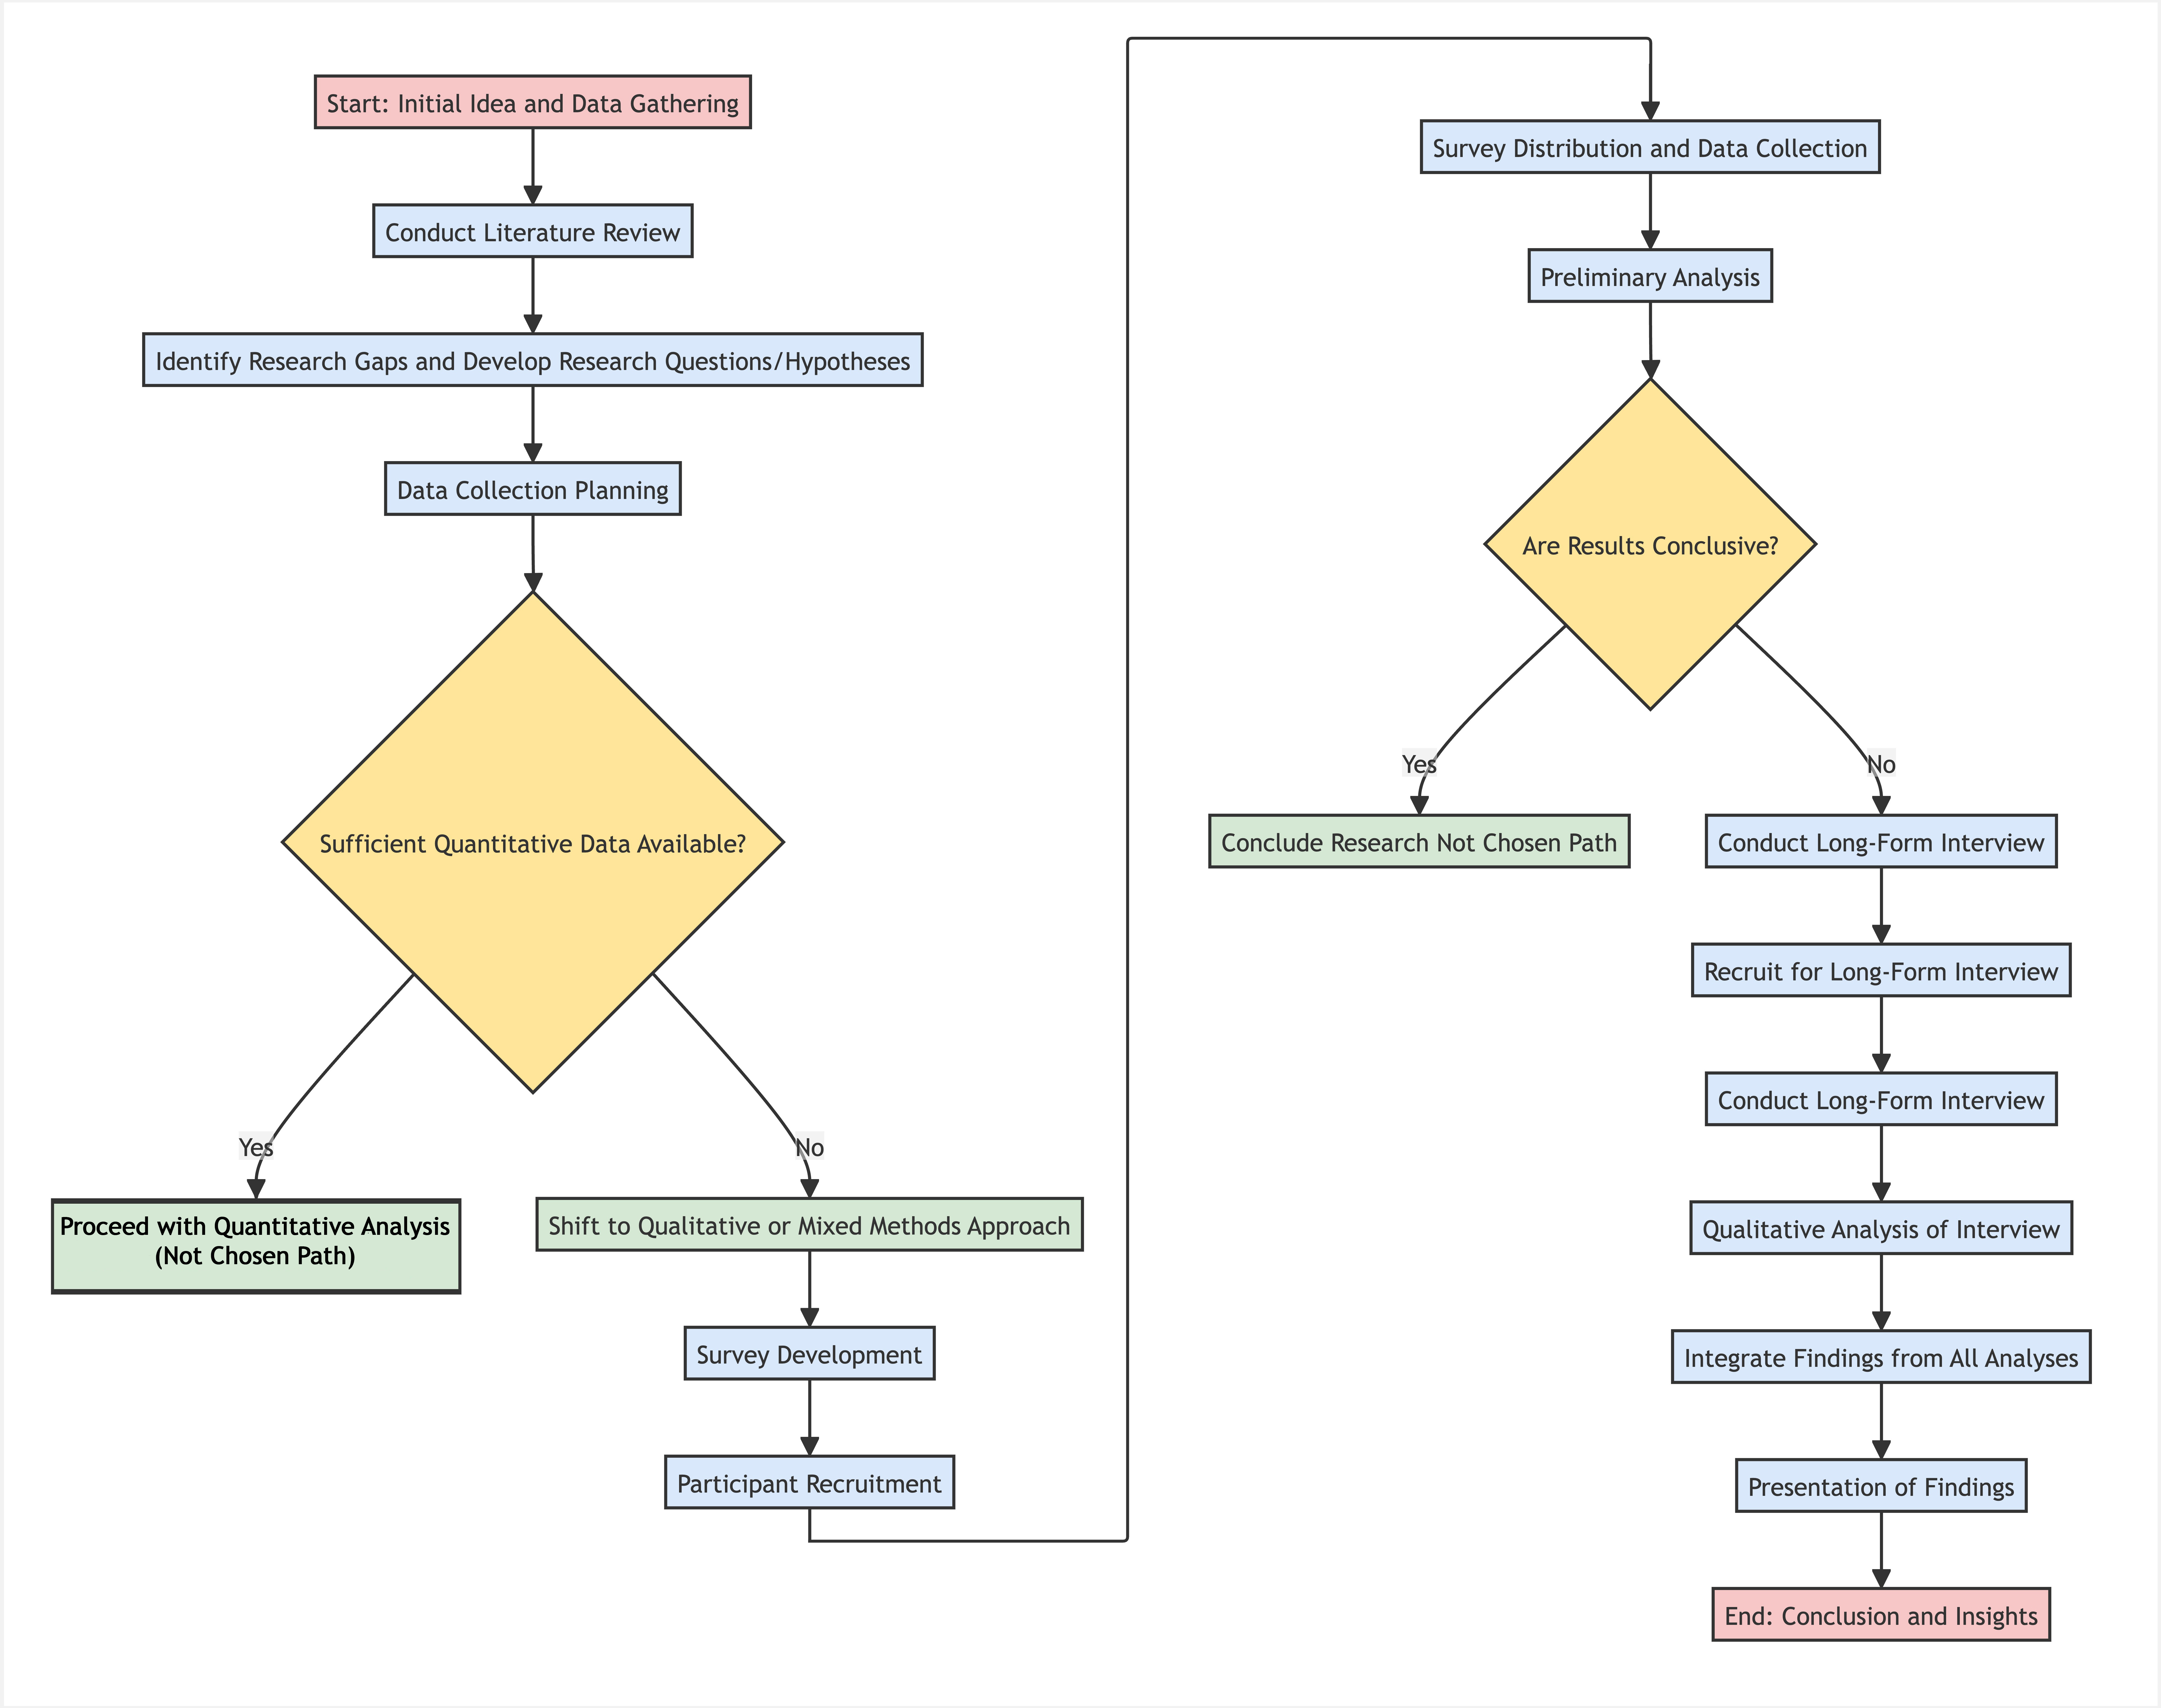
\includegraphics[width=1\textwidth]{figure/research_process.jpg}
  \caption{The research process.}
  \label{fig:research_process}
\end{figure}

\section{The Survey}

\subsection{Format of the survey}
In designing our survey for this study, we utilized a combination of Likert scale questions, yes/no questions, and a single subjective question, as previously mentioned. The Likert scale, a fundamental tool in social science research, was particularly useful for quantifying attitudes, beliefs, and behaviors related to supply chain resilience during the COVID-19 pandemic. By converting qualitative perceptions into quantitative data, it allowed us to perform a robust statistical analysis of these subjective constructs. While Likert scales can vary in length, we chose a 5-point scale (ranging from Strongly Agree to Strongly Disagree) to simplify the process for our respondents, thereby reducing their burden and encouraging higher completion rates. 

Our approach involved careful consideration of the number and type of questions included in the survey. Although it is common to use extensive Likert-scale questionnaires for detailed statistical analysis, we opted to limit the number of these questions to three, recognizing the low response rate and the need to maintain participant engagement. This decision was influenced by the initial literature review, which indicated that reducing the complexity of the survey could lead to more reliable data collection. The yes/no questions were strategically included to provide clear, straightforward insights into whether companies had implemented measures to address specific supply chain challenges, without delving into the success or failure of those measures. To develop the Likert scale questions, we conducted a thorough review of current topics in supply chain management, with a focus on resilience and challenges during the pandemic, as highlighted in several key publications. These questions were designed to be clear, concise, and free from bias, each aiming to capture the respondents' level of agreement or disagreement with statements reflecting critical aspects of their internal processes. 

The layout of our survey was meticulously crafted to minimize confusion and bias. We ensured that instructions were clear and emphasized that there were no right or wrong answers, which was crucial for maintaining the anonymity and confidentiality of respondents. This approach was intended to foster honest and thoughtful responses. The inclusion of a single open-ended question at the end of the survey allowed participants to provide additional insights or recommendations, adding a qualitative dimension to our analysis. In terms of administration, the survey was conducted online to maximize reach and convenience, given the constraints of the pandemic. This method was chosen to increase the response rate and ensure that we collected a representative sample. The combination of Likert scale questions with yes/no questions provided a comprehensive view of supply chain resilience, allowing us to understand not only the existence of specific measures but also the attitudes and thought processes behind them. This mixed-method approach ultimately provided a nuanced understanding of the challenges faced by supply chains during the pandemic.

\subsection{Survey Design and Rationale}

The survey developed for this study was meticulously designed to capture a comprehensive understanding of the impact of the COVID-19 pandemic on supply chain resilience, particularly within the context of perishable goods. Each question was carefully crafted to elicit specific insights while allowing for future in-depth analysis based on the data collected. The rationale behind the selection and formulation of each question reflects our intent to gather both quantitative and qualitative data that can inform broader discussions on supply chain strategies and their efficacy during unprecedented disruptions.

\subsubsection*{Identification of Perishable Goods}
The initial question aimed to categorize the type of perishable goods managed by the respondents' companies. Recognizing the diversity in perishable goods—ranging from vegetables and dairy products to meat, poultry, and seafood—this question was essential for contextualizing the subsequent responses. By allowing participants to select multiple categories, the survey accounted for companies dealing in various types of perishable goods. This categorization facilitated the understanding of industry-specific challenges and also enabled potential comparative analysis across different types of perishable goods. Defining "perishable goods" within the survey ensured that all participants had a consistent understanding, thereby reducing any ambiguity in their responses.

\subsubsection*{Company Turnover and Size}
The subsequent questions concerning the company’s turnover and size were designed to explore the potential correlation between a company’s scale and its response to supply chain disruptions. The turnover question was included to differentiate between small, medium, and large enterprises, allowing us to assess whether financial resources influenced the effectiveness of supply chain strategies during the pandemic. Larger companies, with their broader reach and potentially more complex supply chains, might have different strategies compared to smaller firms with more localized operations. This question set the stage for analyzing whether the scale of operations impacted a company’s ability to adapt to the pandemic-induced challenges. Similarly, the question regarding company size, classified into small (up to 50 employees), medium (51-250 employees), and large enterprises (over 250 employees), was intended to further refine our understanding of how organizational structure and capacity might influence supply chain resilience. By capturing this data, we anticipated the ability to segment responses and explore trends that might differ based on the size of the organization. For instance, larger enterprises might have more formalized strategies and resources, while smaller companies might rely on more agile and ad-hoc approaches.

\subsubsection*{Supply Chain Disruptions and Strategic Responses}
A critical component of the survey involved assessing the extent to which the COVID-19 pandemic disrupted supply chains, specifically for perishable goods. This question utilized a Likert scale, ranging from 1 (not at all) to 5 (very significantly), to capture the severity of the disruption as perceived by the respondents. The use of a Likert scale in this context allowed for a nuanced understanding of the impact, enabling respondents to express varying degrees of disruption. This data is crucial for understanding the scale of the challenge faced by different companies and sets the foundation for analyzing how these disruptions influenced subsequent strategic decisions. Following this, the survey inquired whether the company had implemented any changes to its supply chain strategies during the pandemic. This yes/no question aimed to capture a binary response, providing a clear indicator of whether companies actively adapted their supply chain practices in response to the crisis. This question was followed by another yes/no question regarding whether companies had diversified their supplier base—a common strategy to mitigate risks associated with supply chain disruptions. The sequential nature of these questions was intentional, designed to lead respondents from the recognition of disruption to specific strategic responses, thus creating a logical flow in the survey.

\subsubsection*{Evaluating the Effectiveness of Resilience Strategies}
The survey then probed the effectiveness of the resilience strategies that were in place before the pandemic. Using a Likert scale from 1 (not effective) to 5 (extremely effective), this question sought to gauge how well-prepared companies were to handle the unprecedented challenges posed by the pandemic. By asking participants to evaluate the success of their existing strategies, the survey aimed to identify potential gaps in preparedness and areas where companies may have over or underestimated their resilience. Further, the survey explored whether companies had developed any backup plans for future disruptions. This question, also structured as a yes/no option, was critical in understanding the lessons learned by companies during the pandemic and whether they had proactively taken steps to bolster their supply chain resilience against future crises. The inclusion of this question allowed us to assess the forward-thinking approaches of companies and their commitment to improving resilience post-pandemic.

\subsubsection*{Adjustments in Demand Forecasting and Pandemic Preparedness}
The survey also addressed whether companies had adjusted their demand forecasting methods in response to the pandemic. Accurate demand forecasting is pivotal in supply chain management, especially in times of uncertainty. The question sought to determine if companies had recognized the need for more adaptive forecasting techniques as market conditions rapidly changed during the pandemic. The final structured question asked whether the company had established a formal pandemic preparedness plan for future events. This yes/no question aimed to determine whether the experiences of the COVID-19 pandemic had led to the institutionalization of specific preparedness measures. The presence of such a plan would indicate a company’s strategic shift towards long-term resilience and readiness for potential future disruptions.

\subsubsection*{Subjective Insights from Participants}
To complement the structured questions, the survey included a subjective, open-ended question inviting respondents to share additional insights based on their personal experience of handling supply chain issues during the pandemic. This question was strategically placed at the end of the survey to provide participants with the opportunity to elaborate on any points not covered by the structured questions. It allowed for the collection of qualitative data that could offer deeper insights into the challenges and strategies employed by different companies. This open-ended format included to capture the unique perspectives and innovative solutions that may not have been addressed through the more structured questions.

\subsection{Survey Distribution and Targeting}

The survey for this study was created using Google Sheets, allowing us to generate a shareable link that could be easily distributed to potential participants. The complete set of survey questions can be found in Appendix \ref{appendix:survey}. The focus of our work was narrowed to contain only European countries as we, the authors, are located in European Union member countries and found that this demographic affects us the most. Our focus was exclusively on participants from Europe, reflecting our research's geographic concentration. To identify suitable participants, we conducted extensive research on LinkedIn. We filtered potential contacts by country and then searched for individuals holding prominent positions relevant to supply chain management, such as Purchasing Assistant, Store Manager, Location Manager, and Director of Procurement, among others. 

This approach enabled us to target professionals directly involved in supply chain operations across various European countries. The companies selected were among the top 5 chain supermarkets in countries with the highest GDP in the Union. Some of the countries selected are such but not limited to Sweden, Norway, Czech Republic, the Netherlands, England, Spain, Germany, and etc. This ensured that we take samples of countries with different Geo-locations. As can be seen, some countries are Nordic, which are larger landmass countries with scarcely populated cities, where other countries such as the Netherlands, Spain, and France are evenly populated or almost densely populated areas. 

After identifying potential participants on LinkedIn, we initiated contact primarily through LinkedIn messaging. In cases where contact details were not readily available, we supplemented our efforts by sending emails. For those whose emails were not publicly available, we employed a common email format (first name dot last name at the company's domain) to reach out to them. We ensured that participants were informed that their responses would remain anonymous, with no personal details being recorded. This information was clearly communicated in both the LinkedIn messages and emails sent to potential respondents. 

Additionally, we emphasized that participation in the survey was entirely voluntary, with no mandatory questions. This approach was designed to make it easier for participants to complete the survey, even if they chose not to answer every question. Understanding that respondents might be reluctant to spend significant time on surveys, we streamlined the process by designing the entire survey to fit on a single page, eliminating the need for a "next" button. Despite the absence of incentives such as prize money or other benefits, we encouraged participation by emphasizing the importance of their input in our research. In total, we targeted participants from 16 European countries and successfully contacted approximately 275 individuals across a range of supermarkets, including Netto, Coop, Lidl, Kiwi, Aldi, Carrefour, and more. For a detailed breakdown of the number of people contacted, the countries involved, the supermarkets represented, and the typical positions targeted, please refer to Table \ref{tab:survey-participants}.



\begin{table}[H]
\scriptsize
\centering
\begin{tabular}{@{}|l|l|l|l|@{}}
\toprule
\textbf{Country} & \textbf{\begin{tabular}[c]{@{}l@{}}Number of \\ People \\ Contacted\end{tabular}} & \textbf{Supermarkets}                                                                                          & \textbf{Positions}                                                                                                                                                                                             \\ \midrule
Sweden           & 43                                                                                & \begin{tabular}[c]{@{}l@{}}Citigross, Martin \& Cervera, \\ Coop, Hemshop, ICA, Willys, \\ Mathem\end{tabular} & \begin{tabular}[c]{@{}l@{}}Store Manager, Purchasing Assistant, \\ Location Manager, Purchasing \\ Manager, Perishable Purchaser\end{tabular}                                                                  \\ \midrule
Norway           & 9                                                                                 & Kiwi, Coop                                                                                                     & \begin{tabular}[c]{@{}l@{}}Store Manager, Purchaser, Head of \\ Indirect Procurement, Senior \\ Strategic Buyer\end{tabular}                                                                                   \\ \midrule
Denmark          & 19                                                                                & Netto, Coop, Lidl                                                                                              & \begin{tabular}[c]{@{}l@{}}Senior Buyer, Category Manager, \\ Purchasing Assistant, \\ Category Director\end{tabular}                                                                                          \\ \midrule
Finland          & 4                                                                                 & S-Market, K-Supermarket, Lidl                                                                                  & \begin{tabular}[c]{@{}l@{}}Junior Purchasing Manager, \\ Purchasing and Sales Director\end{tabular}                                                                                                            \\ \midrule
Belgium          & 19                                                                                & Aldi, Carrefour, Lidl, Colruyt                                                                                 & \begin{tabular}[c]{@{}l@{}}Senior Buyer, Head of Sales \\ and Purchasing, Technical \\ Purchasing Manager, Reverse \\ Logistics Manager\end{tabular}                                                           \\ \midrule
Netherlands      & 15                                                                                & Albert Heijen, Aldi, Lidl                                                                                      & \begin{tabular}[c]{@{}l@{}}Manager Procurement, \\ Purchasing Manager, \\ Senior Director Procurement\end{tabular}                                                                                             \\ \midrule
Spain            & 34                                                                                & \begin{tabular}[c]{@{}l@{}}Marchedona, Carrefour, Lidl, \\ Aldi, Supercore\end{tabular}                        & \begin{tabular}[c]{@{}l@{}}CSR Manager, IT Procurement \\ Manager, Senior Buyer, Indirect \\ Purchasing VP, \\ Supply Chain Manager\end{tabular}                                                               \\ \midrule
Portugal         & 18                                                                                & \begin{tabular}[c]{@{}l@{}}Pingo Doce, Continente, \\ Intermarche\end{tabular}                                 & \begin{tabular}[c]{@{}l@{}}Category Manager, National Retail \\ Operations Director, Store Manager, \\ Digital Channels Director\end{tabular}                                                                  \\ \midrule
France           & 18                                                                                & \begin{tabular}[c]{@{}l@{}}Carrefour, Intermarche, \\ Monoprix\end{tabular}                                    & \begin{tabular}[c]{@{}l@{}}Global Category Management, \\ International Head of Buying, \\ Import Director, Director of \\ Supply Chain, Trader\end{tabular}                                                   \\ \midrule
Greece           & 9                                                                                 & \begin{tabular}[c]{@{}l@{}}Sclavenitis, Alpha Beta \\ Vassilopoulos\end{tabular}                               & \begin{tabular}[c]{@{}l@{}}Category Manager, Buyer, Logistic \\ Project Manager, Warehouse Manager\end{tabular}                                                                                                \\ \midrule
Switzerland      & 27                                                                                & Denner, Migros, Aldi                                                                                           & \begin{tabular}[c]{@{}l@{}}Logistic B. Denner, Product \\ Manager, Senior Group Category \\ Director, Buying Director, Country \\ Managing Director, Manager, \\ National Supply Chain Management\end{tabular} \\ \midrule
Italy            & 20                                                                                & \begin{tabular}[c]{@{}l@{}}Conad, Gruppo Selex, \\ Eurospin\end{tabular}                                       & \begin{tabular}[c]{@{}l@{}}Category Manager, Director Supply \\ Chain, National Category Manager, \\ Logistics Manager, Buyer, \\ Logistics Specialist\end{tabular}                                            \\ \midrule
Austria          & 14                                                                                & Rewe, Hofer                                                                                                    & \begin{tabular}[c]{@{}l@{}}Senior Category Manager, Head of \\ Shift Logistic, Procurement Manager, \\ Buying Manager, Buying Specialist, \\ Group Director at Supply \\ Chain Management\end{tabular}         \\ \midrule
Czech Republic   & 10                                                                                & Albert, Tesco                                                                                                  & \begin{tabular}[c]{@{}l@{}}Head of Supply Chain, Supply Chain \\ Manager, Director of Strategic Sourcing, \\ Buying and Merchandising Director\end{tabular}                                                    \\ \midrule
Poland           & 13                                                                                & Eurocash, Zabka                                                                                                & \begin{tabular}[c]{@{}l@{}}Supply Chain Planning Manager, \\ Senior Supply Chain Manager, \\ Logistics Controlling Manager, \\ Logistics Operation Manager\end{tabular}                                        \\ \midrule
Slovakia         & 3                                                                                 & Tesco                                                                                                          & \begin{tabular}[c]{@{}l@{}}Stock Controller Coordinator, \\ Big Data Analyst for Supply \\ Chain, Supply Chain Promotion Manager\end{tabular}                                                                  \\ \bottomrule
\end{tabular}
\caption{Number of people contacted for the survey. Total number of contacts - 273. Total responses - \participantCount}
\label{tab:survey-participants}
\end{table}

When we encountered challenges in gathering sufficient responses for our study on supply chain resilience, especially from experts in specialized fields, we found that a multi-faceted approach was necessary. We expanded our reach by leveraging our extended professional networks through platforms like LinkedIn. We urged our first or second circle contacts to reach out to their contacts and help us with the surveys and finally, we picked up the phone and tried to reach those individuals through company reception numbers and cold-calling professionals at their office numbers within our local country and beyond. Additionally, we utilized  social media forums and professional networks to connect directly with potential participants.  These strategies significantly enhanced our ability to collect the necessary data efficiently  enabling the accumulation of sufficient data to conduct a substantive analysis, ensuring that the qualitative research met statistical validity and reliability criteria.

% \label{sec:pls-sem}

\subsection{Methodology for Survey Analysis}

Data analysis is a critical component of research across various domains, providing essential insights and driving informed decision-making. As data complexity and volume continue to grow, so does the need for sophisticated techniques to analyze and interpret this data effectively. This section explores several prominent data analysis techniques used in contemporary research, followed by an in-depth discussion of Partial Least Squares Structural Equation Modeling (PLS-SEM). We will conclude with a rationale for choosing PLS-SEM as the most suitable method for our thesis. 

\subsubsection{Data Analysis Techniques}

The field of data analysis encompasses a wide range of techniques and methods designed to extract meaningful insights from complex datasets. These techniques serve various analytical purposes, from understanding fundamental patterns in data to developing sophisticated predictive models. Given the diversity of data types, research objectives, and contexts in which data is analyzed, selecting the appropriate method is crucial for achieving reliable and valid results. This section provides a concise overview of several key data analysis techniques commonly employed in academic and professional research. Each method offers unique advantages and is suited to specific types of data and research questions, contributing to the robust analysis and interpretation of data in various domains.

\begin{description}[font=\normalfont\itshape]
    \item[\textit{\textbf{Descriptive Statistics}}] Descriptive statistics provide a foundational understanding of data by summarizing its main characteristics through measures such as mean, median, mode, and standard deviation. These statistics are essential for preliminary data analysis, offering a snapshot of data distribution and variability \parencite{Mann2018IntroductoryStatistics}.

    \item[\textit{\textbf{Regression Analysis}}] Regression analysis is a powerful technique used to understand the relationship between dependent and independent variables. It includes various forms such as linear regression, logistic regression, and multiple regression, each serving specific analytical needs \parencite{Montgomery2021IntroductionAnalysis}.

    \item[\textit{\textbf{Factor Analysis}}] Factor analysis is used to identify underlying relationships between measured variables. It helps in data reduction by grouping variables into factors based on their correlations, making complex data more manageable and interpretable \parencite{Andy2018DiscoveringStatistics}.

    \item[\textit{\textbf{Cluster Analysis}}] Cluster analysis involves grouping a set of objects in such a way that objects in the same group (or cluster) are more similar to each other than to those in other groups. This technique is widely used in market research, pattern recognition, and bioinformatics \parencite{Hair2019WhenPLS-SEM}.

    \item[\textit{\textbf{Time Series Analysis}}] Time series analysis focuses on analyzing data points collected or recorded at specific time intervals. Techniques such as ARIMA and Exponential Smoothing are used to forecast future trends based on historical data \parencite{Box2015TimeControl}.

    \item[\textit{\textbf{Partial Least Squares Structural Equation Modeling (PLS-SEM)}}] \hfill \\
    PLS-SEM is a multivariate statistical analysis technique used to analyze complex relationships among variables. It is particularly useful for predictive modeling and theory building in situations where the data is not normally distributed or the sample size is small \parencite{Sarstedt2017PartialModeling}.
\end{description}

\subsubsection{PLS SEM for Research}

Partial Least Squares Structural Equation Modeling (PLS-SEM) is a powerful statistical technique and a second-generation multivariate method gaining traction in various research fields, particularly in social sciences, business research, marketing, and information systems. It allows researchers to construct and test complex models involving multiple latent and observed variables and is particularly useful for models with numerous variables, intricate relationships, and multiple indicators for each variable \parencite{Sarstedt2017PartialModeling, Henseler2015AModeling}. PLS-SEM helps researchers analyze the interplay between multiple variables, including those not directly measurable (latent variables), thereby providing a deeper understanding of cause-and-effect relationships in complex systems \parencite{Sarstedt2017PartialModeling}. Unlike Covariance-Based SEM (CB-SEM), PLS-SEM focuses on maximizing the explained variance of dependent constructs, making it an ideal choice for predictive modeling, theory development, and exploratory research \parencite{Chin1998TheModeling} \parencite{Sarstedt2017PartialModeling}. In contrast to techniques focused on confirming existing theories, PLS-SEM is particularly suited for developing new theories or extending existing ones, especially when the goal is to predict or identify key factors influencing a phenomenon \parencite{Chin1998TheModeling}. PLS-SEM thrives in contexts where data complexity is the norm, such as in studying intricate systems like family businesses or large-scale marketing campaigns \parencite{Henseler2015AModeling}. PLS-SEM's robustness and flexibility allow it to handle challenging data conditions that traditional methods may not manage effectively. It accommodates both reflective and formative measurement approaches, offering the flexibility to choose between indicators that either reflect or form the underlying concept, depending on the research question \parencite{Chin1998TheModeling}. 

This method is advantageous in dealing with real-world data that does not always follow a perfect normal distribution, making minimal assumptions about the underlying data distribution \parencite{Lohmoller1989LatentSquares}. It also supports the evaluation of theoretical models, even with smaller sample sizes, unlike other techniques that require larger samples for accuracy \parencite{Sarstedt2017PartialModeling}. The methodology has gained popularity in fields such as marketing, information systems, and social sciences due to its capacity to model intricate relationships and assess the reliability and validity of constructs, even with small samples and non-normal data distributions \parencite{Chin1998TheModeling}. 

It effectively tackles common challenges in social science research, making it particularly suitable for complex models where data may be limited or challenging to collect. Moreover, PLS-SEM has been highlighted as a robust solution in evaluating theoretical models in the social sciences, business research, and other fields where data complexity is prevalent \parencite{Sarstedt2017PartialModeling}.

PLS-SEM is well-suited for exploratory research and prediction-oriented studies due to its focus on maximizing the explained variance of the dependent variables \parencite{Henseler2015AModeling}. Unlike traditional covariance-based SEM methods, which often require larger sample sizes and confirmatory analysis, PLS-SEM provides a reliable alternative for research scenarios that demand flexibility and adaptability in dealing with diverse data structures and research objectives.

\paragraph{Key Features of PLS-SEM}

PLS-SEM prioritizes prediction, making it suitable for exploratory research where theory is less developed.It is capable of handling both reflective and formative measurement models \parencite{Chin1998TheModeling}. It is effective with small to medium sample sizes, which is often a limitation in other SEM approaches \parencite{Sarstedt2017PartialModeling}. It is robust against deviations from normality, allowing for broader applicability across different datasets \parencite{Henseler2015AModeling}. Additionally, PLS-SEM offers a valuable toolkit for researchers navigating complex relationships and data limitations. Its ability to handle intricate models, work with small samples, and provide flexibility in measurement makes it a compelling choice for various research endeavors \parencite{Tenenhaus2005PLSModeling}.

\paragraph{Steps in PLS-SEM}

\begin{itemize}
    \item \textbf{Model Specification}: Define the structural and measurement models. The structural model (inner model) specifies relationships between latent variables, while the measurement model (outer model) links latent variables to their indicators \parencite{Lohmoller1989LatentSquares}.

    \item \textbf{Model Identification}: Ensure the model is identified with sufficient data points to estimate parameters.

    \item \textbf{Data Collection}: Gather data for all observed variables.

    \item \textbf{Model Estimation}: Use the PLS algorithm to estimate path coefficients, weights, and loadings \parencite{Wold1985SystemsSquares}.

    \item \textbf{Model Evaluation}: Assess the model using criteria such as convergent validity, discriminant validity, composite reliability, and R² values \parencite{Tenenhaus2005PLSModeling}.

    \item \textbf{Model Interpretation}: Interpret the results to draw meaningful conclusions about the relationships between constructs.
\end{itemize}

\paragraph{Model Evaluation Criteria}

\begin{itemize}
    \item \textbf{Convergent Validity}: Assessed through Average Variance Extracted (AVE), which should exceed 0.50 \parencite{Henseler2015AModeling}.

    \item \textbf{Discriminant Validity}: Evaluated using the Fornell-Larcker criterion, where the AVE of each construct should be greater than the squared correlations with other constructs \parencite{Henseler2015AModeling}.

    \item \textbf{Composite Reliability}: Should be above 0.70 to ensure reliability of constructs \parencite{Sarstedt2017PartialModeling}.

    \item \textbf{R\textsuperscript{2} Values}: Indicate the amount of variance in the dependent variables explained by the model.
\end{itemize}

\paragraph{Motivation for Using PLS-SEM}

The choice of PLS-SEM for our research is motivated by several key factors that align with the nature of our dataset and research objectives. Our research model, while not overly complex, involves three key constructs that require a nuanced analysis of relationships and interactions. PLS-SEM is particularly suited for this type of model, as it allows us to efficiently explore the connections between these constructs without being restricted by the limitations of simpler modeling techniques. Moreover, our study seeks to understand the relationships between pandemic-induced disruptions, change management practices, and resilience strategies, necessitating a method that can simultaneously assess both the measurement model (which evaluates the reliability and validity of constructs) and the structural model (which examines the relationships between constructs). This dual focus is critical for addressing our research questions, particularly given our initial assumptions about the significance of resilience strategies prior to the survey.

Additionally, PLS-SEM offers flexibility in handling low variance data, which is particularly relevant given the minimal variance observed in our responses; traditional methods that depend on maximizing explained variance would not be suitable in this context. Instead, PLS-SEM enables us to model and interpret the structural relationships effectively, even when the variance explained by the model is low, emphasizing the estimation of path coefficients and identifying key drivers. The method's robustness to data and sample size constraints also makes it ideal for our study, as our dataset is moderately sized and may not meet the stringent requirements of other SEM techniques that rely on larger sample sizes and normal data distributions. Furthermore, PLS-SEM is particularly suited for exploratory research, allowing us to uncover new insights and develop theoretical models. Given that our primary aim was to explore potential relationships between constructs rather than confirm them definitively, PLS-SEM serves as an appropriate and reliable choice for our analysis.

\noindent In conclusion, PLS-SEM offers a valuable toolkit for researchers navigating complex relationships and data limitations. Its ability to handle intricate models, work with small samples, and provide flexibility in measurement makes it a compelling choice for various research endeavors \parencite{Tenenhaus2005PLSModeling}.

\subsection{Keyword Extraction for Open-Ended Question}

As discussed previously, we have introduced one open-ended question within our survey, namely: (Refer the entire questionnaire in Appendix \ref{appendix:survey}).

\begin{tcolorbox}[colback=blue!5!white, colframe=blue!15!black, boxrule=0.5mm, title=Subjective Question, fonttitle=\bfseries]
  We would really appreciate it if you can add some insights based on your personal experience of handling supply chain issues during the pandemic.
\end{tcolorbox}

Due to the nature of this question, a different approach was needed to analyse all the responses. While we have engaged in a thorough qualitative examination of the subjective responses—employing a traditional interpretative approach to manually read and derive inferences from the survey data—our analysis did not stop there. Recognizing the value of quantifiable insights in enhancing the reliability and generalizability of our findings, we subsequently applied statistical methods to analyze these responses. This dual approach enabled us to capture the nuanced perspectives offered by the respondents, and also to quantify patterns and trends that could be systematically validated. In this section we will discuss the quantitative methodology employed by us. 

There are various recognised methodologies that are used to analyse subject data. \textcite{Joshi2024AAnswers} have analysed various methodologies that are used to perform automated assessment for subjective responses as we have received in our questionnaire. Content Analysis \parencite{Harwood2003AnAnalysis}, which is a systematic technique for interpreting textual data by categorizing the content into various groups based on specific criteria. While it can be both qualitative and quantitative, often the frequency of words, phrases or topics are counted to identify patterns or trends. Another prominent methodology, Thematic Analysis \parencite{terry2017thematic} predominantly qualitative and focuses on identifying and analyzing patterns or themes within data. It involves closely reading the text to code data and sort these codes into themes that emerge organically. It's flexible and can uncover rich, detailed, and complex data interpretations. 

Discourse Analysis \parencite{gill2000discourse}, while defined differently in many literature, generally goes beyond the content of text to consider the context and means of communication. It examines how language is used in the text to convey messages, and how this relates to social and cultural contexts. In addition, another prominent method, Grounded theory \parencite{birks2015grounded_ch1} is used to generate or discover a theory through the data collected. It involves collecting data and analyzing it iteratively. As more data is collected, and analysis proceeds, the emerging theory or conceptual framework starts to take shape. This method is particularly useful for new areas of research where existing theories might not apply. Another prominent methodologies are Sentiment Analysis \parencite{Wankhade2022AChallenges}, Lexical Analysis \parencite{Bolden2000BridgingDivide}, Narrative Analysis \parencite{Burck2005ComparingAnalysis}, Machine Learning Techniques \parencite{Jain2021AReviews, Alantari2022AnReviews} and Keyword Extraction.

Keyword Extraction \parencite{Firoozeh2020KeywordMethods, Bharti2017AutomaticSurvey} is a broad umbrella that includes various automatic and manual methodologies that prominently focuses on extracting keywords from subjective texts. \textcite{Yuan2018TextStrategy} describe some prominent Keyword Extraction algorithms. TF-IDF (Term Frequency-Inverse Document Frequency) is about weighting the frequency of a word in a document against its frequency across all documents to identify its importance, while LDA (Latent Dirichlet Allocation) is a probabilistic model that identifies topics distributed across a corpus of texts and assigns keywords to these topics based on their distribution, furthermore, TextRank is a graph-based ranking model for text processing which forms a network from the text and uses the structure of this network to determine the importance of words or phrases. 

Building on the array of methodologies previously described for analysing textual responses, our approach used in this study diverges somewhat from conventional automated techniques. Insted of deploying established algorithms such as TF-IDF, LDA, or TextRank, we adopted a manual extraction method. This methodological choice was chosen on several key considerations. Firstly, the manageable scope of the dataset - comprising of \participantCount{} responses, each encapsulated within two to three sentences - rendered manual analysis both feasible and practical. This hands-on approach ensured we understand the overall theme of the response, and that we can perform nuanced comprehension and interpretation, which could easily be missed by employing any simple text parsing or word frequency analysis tools/algorithms. For instance, different respondents might articulate similar sentiments or ideas using disparate linguistic expressions, something that purely automated systems could potentially overlook. 

This manual method, could possibly be categorised, or partially categorised under various analytical paradigms. It shares affinities with \textit{content analysis} in its meticulous parsing of text to identify key terms; and with \textit{thematic analysis} in its sensitivity to underlying themes conveyed across all responses. This technique, however, does not align strictly with any single established methodology like \textit{sentiment analysis} or \textit{discourse analysis}, although it incorporates elements of these through its interpretative elements. The decision to abstain from fully automated methods was also taken due to the desire to preserve the integrity and depth of qualitative data, ensuring that the richness of the respondents' expressions was fully captured and reflected in the analysis. 

In our approach of keyword extraction, our methodology entailed a meticulous manual review of each response. We initiated this process by reading through the first entry comprehensively, extracting prominent keywords that capture the the essence of the respondents' perspectives. Some noteworthy keywords involve "\textit{diversified supplier base}", "\textit{demand forecasting}" and "\textit{strengthening supply ties}". This will be discussed in detail in further sections. It is important to note that the response need not contain the exact phrase of \textit{diversified supplier base}; however, if the respondent talks about diversifying their supplier base in any other way, we have used the a common and popular term that could explain their sentiments in our extraction. The same process is employed in extraction any other keywords from the answer. Subsequent to this extraction, we engage in an iterative review process, where we similarly analyse the next response. If this response discusses something that aligns with any of the existing keywords, we increase the frequency of those keywords by one, meanwhile also trying to extract any more prominent keywords from the response. We keep doing it for all \participantCount{} responses and thus, end up with a list of keywords and their frequencies. Note that the entire process is performed manually by reading through each responses. Eventually, from the list of all available keywords, most frequent keywords are then chosen for any further analysis. Figure \ref{fig:kye_extraction} diagrammatically describes the entire keyword extraction process used.

\begin{figure}[ht]
  \centering
  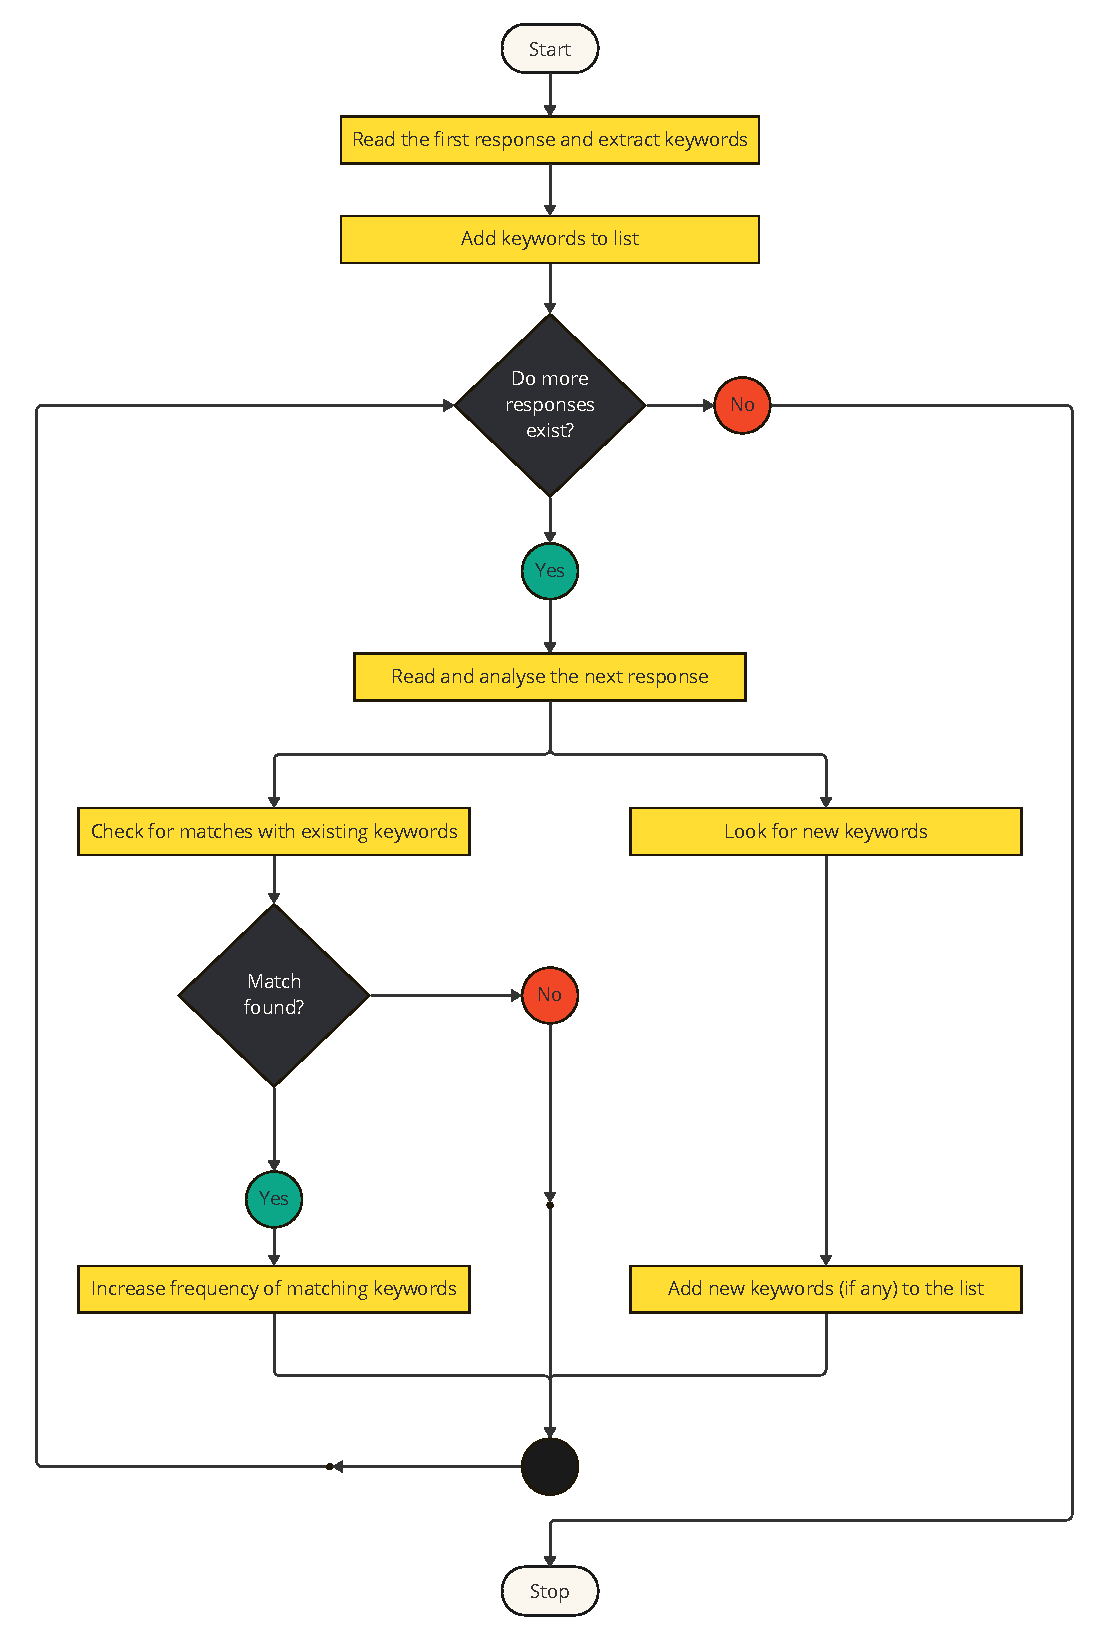
\includegraphics[width=0.6\textwidth]{figure/keyword_extraction_flowchart.pdf}
  \caption{Flowchart of the keyword extraction methodology employed.}
  \label{fig:kye_extraction}
\end{figure}


\subsection{Limitations and Ethical Considerations}

We ensured the ethical treatment of all participants throughout the research process, strictly adhering to GDPR guidelines to protect personal data and privacy. In line with these regulations, we made certain that no personal data was recorded at any stage of the survey. Participants were informed from the outset that their responses would remain completely anonymous, and we explicitly stated that no identifiable information would be collected. This was done to maintain the confidentiality of the data and to ensure participants felt secure in providing honest responses. Participation in the survey was entirely voluntary, with no questions marked as mandatory. This approach was designed to respect the autonomy of the respondents, allowing them to skip any questions they were uncomfortable answering without affecting their ability to submit the survey. 

Additionally, we offered participants the option to engage in a follow-up interview for more in-depth discussion. This option was also presented as entirely voluntary, and participants were given the choice to provide their contact details only if they were interested in participating further. This approach allowed us to gather richer qualitative data from those who were willing, while still respecting the privacy of those who chose not to engage further. One of the key limitations of our study was the decision not to record any identifying information about the participants, in order to comply with ethical standards and data protection regulations. While this ensured the anonymity and confidentiality of the respondents, it also introduced a significant limitation: we were unable to link responses back to specific individuals, countries, companies, or job positions. 

This lack of granularity in the data meant that while we knew which countries, companies, and positions were targeted, we could not directly associate specific responses with these variables. Consequently, our analysis could not account for potential differences in responses based on these factors, which may have provided additional insights into the impact of the pandemic on different segments of the supply chain. Another limitation was related to the survey design itself. Initially, we developed a more extensive set of questions, which we sent to a small group of known contacts for feedback. The feedback indicated that the survey was too lengthy, particularly given that participation was voluntary and there were no incentives offered. 

Respondents expressed reluctance to complete a long survey, which led us to significantly shorten the questionnaire. The final survey consisted of only 10 questions, with only 7 designed for quantitative analysis and 1 for qualitative analysis. This reduction in the number of questions limited the depth of the data we could collect, particularly in terms of more focused or detailed inquiries that might have provided richer insights. The trade-off, however, was an increased likelihood of participation, which was crucial given the challenges of obtaining responses without offering incentives.

Thus, while we took significant steps to ensure the ethical treatment of participants and to protect their privacy, these measures also introduced limitations in the scope and depth of our analysis. The constraints imposed by the need for anonymity, the voluntary nature of the survey, and the decision to limit the number of questions all impacted the breadth and specificity of the data collected. It should be noted that these limitations are acknowledged and should be considered when interpreting the findings of this study.

\section{The Interviews}

In our research, following the initial survey phase, we recognized the need for a more in-depth qualitative exploration to complement the limited data obtained (will be discussed in further sections) from the survey responses. The objective of this next methodological step was to conduct personal interviews with professionals who could offer deeper insights into the functioning of supply chains during the COVID-19 pandemic and the subsequent adjustments made in response to the challenges faced. Given the lower-than-expected response rate to our survey, despite our efforts to streamline the questions and ensure their relevance and ease of completion, we decided to pursue interviews as a means to bolster our research findings. 

Although our survey was carefully designed to minimize respondent burden—featuring voluntary participation, non-mandatory questions, and a concise structure—we observed that the engagement was insufficient to draw comprehensive conclusions from the quantitative data alone. To address this limitation and enhance the robustness of our research, we moved forward with conducting personal interviews. The initial plan to recruit interview participants involved leveraging the same pool of respondents from our survey. As previously mentioned, we included a question in the survey asking if participants were willing to engage in a follow-up interview for a more detailed discussion. Unfortunately, none of the survey respondents expressed interest in participating further, leaving us without candidates from the survey pool.

Consequently, we had to pivot our approach by once again reaching out to our professional networks, particularly through LinkedIn and other channels, to identify individuals who met the specific criteria required for the interview. It was essential that the interviewee had significant experience in the perishable goods sector and a background in supply chain management. This criterion was crucial to ensure that the insights provided during the interview were both relevant and valuable to our research. Consequently, this requirement also narrowed down people we could contact for the interview. After extensive outreach, we were able to secure a single interview with a participant whose qualifications were highly pertinent to our study. The individual in question had two years of direct experience in supply chain management at Nestlé, a leading company in the perishable goods industry. 

Additionally, the participant had professional experience with financial institutions such as S\&P. Academically, the interviewee held a master's degree in both finance and supply chain management, and a PhD in logistics supply chain, albeit with a focus on construction transport. At the time of the interview, the participant was employed as a Supply Chain Design Specialist at Volvo, adding a layer of credibility to the insights they provided.

% -------------------

Upon receiving agreement from the selected participant, one of the authors conducted the interview via an online Zoom meeting. Prior to the interview, the participant was fully informed of all ethical considerations, including the assurance that no personal data or personal information would be recorded or shared. The interview was conducted under the condition of anonymity, with the understanding that the participant's credentials would be disclosed to demonstrate their credibility and qualifications, but only with their explicit permission. The questions posed during the interview were carefully crafted based on the analysis of the survey data. Specifically, the questions were derived from the analysis of the multiple-choice questions using the PLS-SEM method, which will be elaborated upon in Section \ref{sec:pls-sem}, and from keyword analysis of the responses to subjective questions, as discussed in Section \ref{sec:keyword-analysis}. 

This ensured that the interview questions were directly relevant to the key points identified in the survey and allowed us to explore them in greater depth. In total, approximately 30 questions were prepared for the interview. However, it was understood that this list would serve as a flexible outline rather than a rigid script. The interview was designed to be conversational, allowing for the possibility of skipping certain questions or adding new ones depending on the flow of the discussion. Although no follow-up questions were pre-determined, the interview process included spontaneous follow-up questions to delve deeper into the insights provided by the participant. 

This flexibility was crucial in allowing the interviewer to explore the participant's responses more thoroughly and to gather more nuanced data. The questions covered a wide range of topics, from specific vulnerabilities within the supply chain to strategies for enhancing collaboration with suppliers and the role of technology in improving supply chain visibility and traceability. For example, one of the questions asked the participant to identify specific vulnerabilities within the supply chain, with a follow-up question probing whether they had encountered health-related problems in the food industry. Another question explored the flexibility and adaptability of the supply chain in responding to changes in demand or supply, with a follow-up asking for a specific example from the participant's experience.

The interview was conducted successfully, and the insights gathered provided valuable qualitative data that supplemented the quantitative findings from the survey. This data will be integrated into the overall analysis to provide a more comprehensive understanding of supply chain resilience during the pandemic. After the interview was completed, the actual list of questions and follow-up questions that were asked was compiled and can be found in Appendix \ref{appendix:interview}. This documentation ensures transparency in our methodology and allows for the replication of the study in future research. 

The interview conducted proved to be invaluable, offering detailed qualitative data that supplemented the limited quantitative results from our survey. The expertise and experience of the interviewee provided a depth of understanding that enriched our analysis, particularly regarding the resilience and adaptability of supply chains in the face of unprecedented disruptions like those caused by the COVID-19 pandemic. The insights gained from this interview will be discussed in further detail in the analysis and findings section of this paper, where we will integrate both the survey data and the qualitative insights to present a comprehensive view of the study's results.

% \todo[inline]{research process subsection to be added, where we summarise chronologically the entire process that was done}

\section{Survey Analysis: PLS-SEM}
\label{sec:pls-sem}

The aforementioned surveys and interviews yielded a total of \participantCount{} survey responses and one in-depth interviews. Current and following sections delineate the analytical methodologies employed to scrutinize the data obtained from these surveys and interviews.

In our study, we utilized SmartPLS 4 \parencite{smartpls2024} to analyze the structural equation model (SEM) based on the survey data collected. The constructs and hypotheses were operationalized through a series of survey questions, each carefully designed to measure specific aspects of the constructs in question. Below, we will elaborate on the process of model construction and the rationale behind the arrows and dependencies depicted in the Figure \ref{fig:constructs}. The survey data comprised questions targeted at measuring three main constructs: Pandemic Disruption, Change Management, and Resilience Effectiveness. Each of these constructs was associated with specific questions from the survey. For Pandemic Disruption, we used Question 4 which assesses the extent to which companies experienced supply chain disruptions due to the pandemic. 

This question serves as a critical indicator of the impact of COVID-19 on operational stability. Change Management was measured using Questions 5, 6, 8, 9, and 10. These questions capture various strategic responses implemented during the pandemic, including changes in supply management strategies, supplier diversification, creation of backup plans, adjustment of demand forecasting methods, and the presence of formal pandemic preparedness plans. These aspects collectively reflect the strategic adaptability and preparedness measures undertaken by companies in response to the pandemic. Resilience Effectiveness was gauged through Question 7, which evaluates the effectiveness of the company's resilience strategies such as inventory management and supplier diversification during the pandemic. This construct provides insights into how well existing strategies mitigated the pandemic's impact. The diagram also incorporates the specific survey questions associated with each construct, denoted by the yellow text boxes. For example, CMQ10, CMQ5, CMQ6, CMQ8, and CMQ9 represent the questions related to Change Management. The arrows pointing towards the Change Management node indicate the reflective measurement model, where each question (indicator) is influenced by the underlying construct. 

PLS-SEM analysis is well suited for various types of research data, some of them being the Likert Scale, which typically is a 5-point scale where respondents indicate their level of agreement or disagreement with a statement. The scales usually range from "Strongly Agree" to "Strongly Disagree", or similar. Likert scales are popular in measuring attitudes, perceptions, and behavioral intentions. It is also suited for Binary or Dichotomous Scales, which are simple yes/no or true/false responses. In our case, the responses for Questions 4 and 7 are in the Likert Scale and the responses for Questions 5, 6, 8, 9 and 10 are within the Binary Scale. This is briefly described below.

\subsection{The analysis process}

\begin{enumerate}

    \item \textbf{Selection of Questions for Analysis:} To apply PLS-SEM, we selected questions 4 to 10 for analysis. These questions were chosen because they are either yes/no questions or questions with answers on a scale ranging from 0 to 5, which are suitable for the PLS-SEM modeling approach.

    \item \textbf{Construct Development:} Constructs are developed based on the questions asked, specifically questions 4-10, to create meaningful hypotheses. Constructs represent the theoretical concepts that underpin the variables of interest in the study.

    \item \textbf{Hypothesis Creation and Validation:} The primary objective is to formulate hypotheses based on the research questions and subsequently validate or invalidate them using the responses received. The validation will be conducted through the results obtained from the PLS-SEM analysis.

\end{enumerate}


\subsection*{Summary:}
\noindent Here we will summarise the aforementioned process.

\begin{itemize}
    \item \textbf{Step 1:} Select objective questions (Questions 4-10).
    \item \textbf{Step 2:} Develop constructs based on the selected questions.
    \item \textbf{Step 3:} Formulate hypotheses related to the developed constructs.
    \item \textbf{Step 4:} Apply PLS-SEM to analyze the data and obtain results.
    \item \textbf{Step 5:} Validate or invalidate the hypotheses based on the analysis results.
\end{itemize}

\subsection{Constructs Developed}

Based on the selected questions, we have developed a total of three constructs by grouping similar questions. Each construct is designed to measure different dimensions of supply chain resilience in the context of the COVID-19 pandemic. The constructs and their corresponding rationale are as follows:

\begin{itemize}

    \item \textbf{Construct 1: Pandemic Disruption}
    \begin{itemize}
        \item \textbf{Question Used:} Question 4
        \item This construct is derived from a question that assesses the extent of disruption experienced by companies in their supply chain due to the pandemic. It serves as an indicator of the overall impact of COVID-19 on business operations and highlights the vulnerabilities within supply chains during this period.
    \end{itemize}

    \item \textbf{Construct 2: Change Management}
    \begin{itemize}
        \item \textbf{Questions Used:} Questions 5, 6, 8, 9, 10
        \item This construct is based on multiple questions that address various changes implemented in response to the pandemic. These include adjustments in management strategies, diversification of suppliers, creation of backup plans, modification of forecasting methods, and the establishment of formal preparedness plans. Together, these questions capture the strategic adaptability and proactive measures adopted by companies to manage pandemic-induced disruptions.
    \end{itemize}

    \item \textbf{Construct 3: Resilience Effectiveness}
    \begin{itemize}
        \item \textbf{Question Used:} Question 7
        \item This construct focuses on evaluating the effectiveness of the resilience strategies employed by companies during the pandemic, such as inventory management and supplier diversification. It provides insights into how well these strategies mitigated the impact of disruptions and contributed to overall supply chain resilience.
    \end{itemize}

\end{itemize}


\begin{figure}[H]
  \centering
  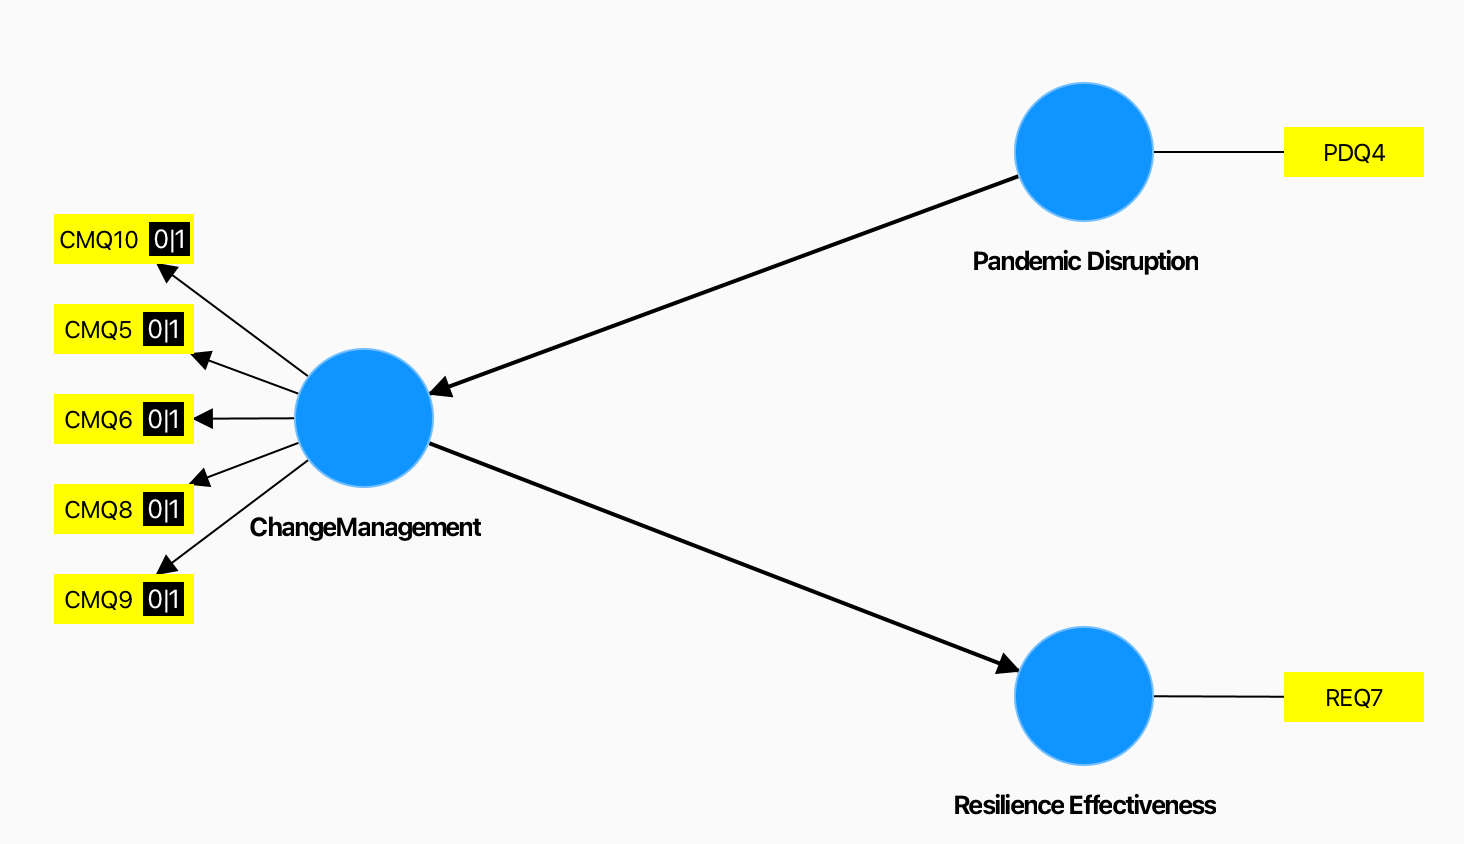
\includegraphics[width=1\textwidth]{figure/initial_model.png}
  \caption{Structural Model in SmartPLS showing the relationships between constructs. The model includes Pandemic Disruption (Q4), Change Management (Q5, Q6, Q8, Q9, 10), and Resilience Effectiveness (Q7). Arrows indicate hypothesized dependencies: Pandemic Disruption's impact on Change Management and Resilience Effectiveness, and Resilience Effectiveness's influence on Change Management. $[0|1]$ Adjacent to the question numbers indicate the binary nature of the questions. Other questions belong to the Likert Scale.}
  \label{fig:constructs}
\end{figure}


\noindent Using SmartPLS 4, we constructed a model (Figure \ref{fig:constructs}) to test our hypotheses. The structural model posits the following relationships:

\begin{enumerate}
    \item \textbf{Pandemic Disruption leads to Change Management (H1)}: This hypothesis suggests that higher levels of disruption due to the pandemic are positively associated with an increase in change management strategies. The arrow from Pandemic Disruption to Change Management in the diagram represents this hypothesis. The rationale is that significant disruptions necessitate strategic changes to adapt and mitigate the impact.

    \item \textbf{Resilience Effectiveness reduces the need for extensive Change Management (H2)}: This hypothesis proposes a negative relationship between the effectiveness of resilience strategies and the extent of change management. If a company’s existing resilience strategies are effective, it may not need to implement extensive changes. This is depicted by the arrow from Resilience Effectiveness to Change Management, indicating that effective resilience strategies can mitigate the need for further change.

    \item \textbf{Pandemic Disruption influences Resilience Effectiveness (H3)}: This hypothesis posits a positive relationship between the level of pandemic disruption and the perceived effectiveness of resilience strategies. Higher levels of disruption may prompt companies to evaluate and enhance their resilience strategies, thus leading to higher effectiveness. This relationship is shown by the arrow from Pandemic Disruption to Resilience Effectiveness in the diagram.

\end{enumerate}

Upon conducting the analysis using the SmartPLS tool for PLS-SEM, we can evaluate the validity of our hypothesized relationships among the constructs. By examining the path coefficients, significance levels (p-values), and the R² values for each endogenous construct, SmartPLS provides comprehensive insights into the strength and significance of the proposed causal paths. In our specific case, this involves assessing whether the hypothesized positive relationship between Pandemic Disruption and Change Management, the negative relationship between Resilience Effectiveness and Change Management, and the positive relationship between Pandemic Disruption and Resilience Effectiveness hold true. 

Additionally, the bootstrapping procedure available in SmartPLS allows us to obtain estimates of standard errors and confidence intervals, further solidifying our hypothesis testing. The evaluation of the model fit indices, such as the SRMR (Standardized Root Mean Square Residual), will help determine the overall adequacy of our model, enabling us to conclude whether the empirical data supports our theoretical propositions. Thus, the detailed results obtained from SmartPLS will enable us to confirm or refute our hypotheses with a considerable degree of statistical confidence. In configuring the SmartPLS software for our PLS-SEM analysis, several key settings were chosen to ensure interpretable results. We selected the Principal Component Analysis (PCA) weighting scheme, a common default choice, as it uses the first principal component of the block’s indicators as the composite score, providing a reliable and standard approach. To facilitate easier interpretation of path coefficients and enable comparisons across constructs, we opted for standardized results, which convert all variables to a common scale. 

For the initial weights, we adhered to the algorithm’s default settings. Regarding the handling of missing values, considering that only one response was partially missing, we utilized casewise deletion, provided it did not significantly reduce our sample size below acceptable limits for robust analysis. Lastly, we did not apply any additional weighting vectors, as none were necessary for our analysis.

\section{Survey Analysis: Keyword Extraction}
\label{sec:keyword-analysis}

The analysis resulted in 10 keywords which were used the most by all our survey-takers. The first round of elimination was to use a cut off of all the words which have less than 5 occurrences. Through this cut off we could make sure that the words that have been chosen for keyword analysis were really the words that had significance for our survey subjects. This resulted in 21 keywords that were chosen for the next round of analysis/elimination. The next round was more based on the context and similarity of the wording used by our survey subjects. For example, words such as "perishable" and "meat and dairy", and/or vegetables are categorized as a single keyword and the frequencies were added to get a cumulative number. Other words such as "demand forecasting" and "strategic foresight" were also put together to add their number of occurrence and shorten our list of keywords. Finally after this process of contextual analysis we ended up with 10 most important keywords which were used by our survey subjects which are stated in Table \ref{tab:keyword-frequency} in order of their significance of occurrence.

\begin{table}[h!]
\centering
\begin{tabular}{|c|c|}
\toprule
\textbf{Keyword} & \textbf{Frequency} \\ 
\midrule
Resilience & 41 \\ 
\hline
Diversified Supplier Base & 30 \\
\hline
Innovation & 27 \\
\hline
Operational Continuity & 26 \\
\hline
Demand Forecasting & 25 \\ 
\hline
Adaptability & 25 \\ 
\hline
Sustainability & 18 \\ 
\hline
Pandemic-induced Supply Chain Disruptions & 13 \\ 
\hline
Agility & 12 \\ 
\hline
Perishables & 12 \\ 
\bottomrule
\end{tabular}
\caption{Frequency of Keywords Related to Supply Chain Resilience}
\label{tab:keyword-frequency}
\end{table}

Using these keywords we came up with 20 i.e. 2 interview questions per keyword to be able to interview our interviewees and understand their input on these significant keywords in our survey and understand their thoughts on these subjects. For this we studied several research papers to come up with interview questions relevant to the topics focused on our keywords \parencite{Tukamuhabwa2015SupplyStudy,Ponomarov2009UnderstandingResilience,Wu2007MethodologyAnalysis,Sawik2017AManagement,Chowdhury2021COVID-19Review}. To be able to prepare for the interview we followed the guidance provided by \textcite{Ghauri2020ResearchStudies} to perform the pre-interview, interview, and post-interview preparation and develop our skills on interviewing our subjects.

\section{Analysis of Long Form Interviews}
\label{sec:intervew-analysis}

The purpose of this interview analysis is to delve deeply into the experiences and insights shared by a supply chain professional to explore the various dimensions of supply chain resilience in the context of the COVID-19 pandemic. By systematically evaluating the interviewee's responses, we seek to validate or invalidate our hypotheses concerning the immediate impacts of the pandemic on supply chains and the strategies implemented by companies to mitigate these impacts and prepare for future crises. The insights gathered from this interview are crucial in validating our hypotheses, specifically those related to the challenges faced by suppliers of perishable goods during the pandemic and the strategies adopted to enhance supply chain resilience. Through the interview, we explore the interviewee's perspective on whether suppliers faced significant disruptions \textit{(Hypothesis 1)}. Additionally, we aim to understand whether these suppliers implemented new strategies to enhance resilience \textit{(Hypothesis 2)}. 
The relevance of this interview is emphasized by the interviewee's substantial experience in managing supply chains for perishable goods. With direct experience in supply chain management at Nestlé, a leading company in the perishable goods industry, and a current role as a Supply Chain Design Specialist at Volvo, the interviewee brings a nuanced perspective that bridges both practical and theoretical knowledge. Their academic qualifications, including a PhD in logistics supply chain and master’s degrees in finance and supply chain management, further enhance the credibility of their insights, particularly concerning complex supply chain dynamics and the need for adaptive strategies during crises. Moreover, the interviewee's background in both the perishable goods sector and broader supply chain management offers a unique vantage point to explore how companies have responded to the disruptions caused by the COVID-19 pandemic.

\subsection{Initial Challenges Faced by Suppliers of Perishable Goods}

The interview reveals several critical challenges that suppliers of perishable goods encountered during the COVID-19 pandemic, which align with the hypotheses proposed in our research. The interviewee described the pandemic period as a time of substantial difficulty, stating, “\textit{it was a great challenge for supply chain management because we have a global supply chain. So it was like really difficult to source the raw material and then send the finished product to the customers}.” This observation supports \textit{Hypothesis 1}, which asserts that suppliers of perishable goods faced significant disruptions in their supply chains due to the pandemic.

\subsubsection{Supply Shortages and Delays in Transportation}

The interviewee highlighted several immediate impacts on supply chains, including supply shortages and delays in transportation. One of the prominent examples mentioned was the incident at the Suez Canal, where “\textit{pirates...stopped the Canal, and it created a big challenge on how to fix it and how to send products through there}.” It is important to note that we could not find any significant incident involving pirates blocking the Suez Canal. However, we assume the interviewee may have mixed it up with the Ever Given incident in 2021, where a massive container ship ran aground, blocking the Suez Canal for nearly a week. This blockage led to a substantial global trade disruption, with an estimated daily loss of \$9.6 billion \parencite{Harper2021SuezDay}, critically affecting regions such as Dubai, where “\textit{all the material goes from that path...that area got critically affected because it got closed down for a long period of time}.” The incident illustrates the vulnerability of supply chains that rely heavily on specific transit routes, supporting the notion that external disruptions, such as geographical bottlenecks, can have a profound impact on the ability of suppliers to meet demand. Furthermore, the interviewee pointed out the complexities associated with managing delays caused by transportation issues. They stated, “\textit{it is really a challenge, like how we can meet the demand and...how much time before you have to place the order to incorporate in-transit time, transport time}.” This statement indicates that unpredictable delays created significant bottlenecks in the supply chain, requiring companies to re-calibrate their logistics and inventory management strategies frequently. These challenges, stemming from transportation delays and route blockages, provide strong evidence for Hypothesis 1, which posits that suppliers experienced considerable disruptions.

\subsubsection{Labor Constraints and Increased Costs}

In addition to supply shortages and transportation delays, labor constraints emerged as a significant challenge during the pandemic. Although the interviewee did not directly elaborate on labor issues, it is implied through their references to challenges in maintaining operations and managing increased costs. The global nature of supply chains meant that suppliers faced difficulties in both “\textit{sourcing the raw material and sending the finished product to the customers},” suggesting disruptions not only in material availability but also in the workforce needed to process and transport these materials. The increased need for labor to manage these disruptions, coupled with constraints due to health and safety regulations, likely resulted in additional costs, further complicating the supply chain management process.

\subsubsection{Comparative Analysis with Hypotheses}

Comparing these accounts with \textit{Hypotheses 1} provides a clear indication that Hypothesis 1 is more strongly supported by the interview data. The interviewee's experiences emphasizes significant disruptions in supply chains due to several factors, including logistical challenges, transportation delays, and supply shortages. Additionally, the arguments posed suggests that suppliers of perishable goods did not experience substantial disruptions. The cumulative impact of incidents like the Suez Canal blockage, coupled with the complexities of global supply chain management during a pandemic, illustrates that the disruptions were indeed significant and widespread.

\subsubsection{Specific Examples Illustrating Disruptions}

Several specific examples from the interview point out the types of disruptions encountered by suppliers. The Suez Canal incident, in particular, serves as a prime example of a transportation-related disruption that significantly affected supply chains. The interviewee mentioned that the closure of the canal had a "critical impact on the Dubai market," and the subsequent difficulty in “\textit{meeting demand}” illustrates the dependency of regional markets on specific supply routes. Moreover, the example highlights how disruptions in one part of the supply chain can have cascading effects across various regions, demonstrating the interconnectedness and fragility of global supply chains. Additionally, the interviewee referred to the broader challenges of managing supply chain operations amid the pandemic, emphasizing the need for “\textit{correct demand forecasting}” to prevent bottlenecks. This statement reflects the inherent difficulty in managing supply chains under uncertain conditions, where disruptions can occur suddenly and unpredictably. The reliance on accurate demand forecasting becomes even more critical in such scenarios to avoid excess inventory or stockouts, further supporting the notion of significant disruptions in supply chains during the pandemic. 

This account provides substantial evidence that suppliers of perishable goods faced multiple initial challenges during the COVID-19 pandemic, including supply shortages, transportation delays, labor constraints, and increased costs. These challenges align closely with \textit{Hypothesis 1}, suggesting that significant disruptions were experienced by suppliers. The examples provided, such as the Suez Canal blockage and regional market dependencies, illustrate the fragility of global supply chains and the cascading impact of localized disruptions. Therefore, the initial analysis strongly supports the argument that the pandemic had a profound and widespread impact on supply chain operations for suppliers of perishable goods.

%===================3rd Section

\subsection{Strategies Adopted by Suppliers During the Pandemic}

The interview provides an overview of both immediate and long-term strategies adopted by suppliers of perishable goods in response to the disruptions caused by the COVID-19 pandemic. These strategies were crucial for maintaining supply chain resilience and ensuring the continuous flow of goods, despite unprecedented challenges.

\subsubsection{Immediate Response Strategies}

The interviewee detailed several short-term strategies employed by suppliers to cope with the immediate disruptions caused by the pandemic. One key strategy was sourcing alternatives, as the interviewee noted, “\textit{it was really difficult to source the raw material and then send the finished product to the customers}.” This difficulty led companies to diversify their supply base to reduce dependency on single sources. The interviewee emphasized the importance of local partnerships, suggesting that “\textit{we should have more supply partnerships in local markets… so our reliance will not become our sole responsibility}.” This reflects a strategic pivot towards sourcing materials from more geographically proximate suppliers, thereby reducing the risk associated with long-distance supply chains.

Additionally, there was a significant focus on using local warehouses to mitigate disruptions in global supply chains. The interviewee mentioned that companies began to “\textit{consider the concept of local warehouses… because they are closer to where things are needed}.” This strategy aligns with \textit{Hypothesis 2}, which posits that suppliers of perishable goods have implemented new strategies and procedures to enhance supply chain resilience. By utilising local warehouses, suppliers could reduce transportation time and costs while increasing the speed of response to sudden changes in demand. The diversification of suppliers also played a critical role in managing risks. 

The interviewee highlighted the benefits of having a combination of large and small suppliers, noting that “\textit{small suppliers are more flexible, whereas larger suppliers are often less adaptable}.” This mix allowed companies to benefit from the flexibility and adaptability of smaller suppliers while still maintaining relationships with larger, more established suppliers for bulk procurement needs. This diversification strategy is consistent with the need for flexibility in responding to disruptions, as outlined in \textit{Hypothesis 2}. Additionally, suppliers enhanced collaboration with both small and large suppliers to manage risks better. As the interviewee noted, “\textit{there should be collaborative partnerships and more involvement of different stakeholders}.” 

This approach enabled suppliers to share risks and responsibilities, fostering a more resilient supply chain network. For example, the interviewee described the increased use of third-party transporters and more flexible transport terms, which allowed suppliers to adapt quickly to changing circumstances. The inclusion of third-party logistics providers facilitated a more agile and responsive supply chain, capable of overcoming sudden transportation challenges or bottlenecks.

\subsubsection{Long-Term Strategic Changes}

In addition to immediate responses, companies made several longer-term strategic changes to enhance supply chain resilience. The interviewee noted that technology adoption became a key focus, with companies looking to integrate technologies such as the Internet of Things (IoT) and Artificial Intelligence (AI) into their supply chains. These technologies were seen as crucial for “\textit{tracking and traceability of the products in real-time},” which is vital for managing perishable goods that require strict monitoring of storage conditions and transportation timelines. The use of IoT and AI could help “\textit{resolve all the bottlenecks and buffer stocks and safety stocks}” by providing real-time data and insights, enabling companies to make more informed decisions quickly. However, it is important to note that the interviewee acknowledged a lack of expertise in computer science or related technical fields, resulting in a limited understanding of AI and IoT. 

Moving on, the interviewee also highlighted the development of new supplier partnerships and a shift towards more comprehensive contingency planning. After the pandemic, many companies began to establish crisis management teams whose “\textit{sole job is to understand and work only on alternative solutions}.” This move illustrates a proactive approach to preparedness, ensuring that companies are better equipped to handle future disruptions. Such investments in crisis management and planning are consistent with \textit{Hypothesis 2}, which suggests that suppliers have implemented new strategies to enhance their resilience.

Additionally, the interview data suggests that several suppliers have indeed made substantial changes, such as adopting new technologies and establishing dedicated crisis management teams. The shift towards technology adoption and the development of new supplier partnerships indicate that companies are actively seeking to enhance their supply chain resilience in preparation for future pandemics or similar disruptive events. The interviewee also discussed the importance of continuous assessment and finding new suppliers to improve terms and conditions and maintain supply chain agility. They stated, “\textit{it is always good to keep looking for new suppliers, innovative ways, and new ways of transporting products}.” This approach reflects a commitment to dynamic supply chain management, where constant evaluation and adjustment are necessary to mitigate risks and respond to changing circumstances.

\subsubsection{Strategies Adopted - Summary}

Thus, the interview reveals that suppliers of perishable goods adopted a range of both immediate and long-term strategies to enhance supply chain resilience during the COVID-19 pandemic. Short-term strategies included sourcing alternatives, local warehousing, supplier diversification, and enhanced collaboration with third-party transporters. Long-term strategic changes focused on technology adoption, new supplier partnerships, and contingency planning. These actions align strongly with \textit{Hypothesis 2}, demonstrating a proactive approach to resilience and preparedness.

%=================SECTION 4

\subsection{Exploring Additional Themes}

\subsubsection{Flexibility and Adaptability of Supply Chains}
The interviewee highlighted the importance of flexibility and adaptability in supply chains, especially in response to uncertain demand changes during the pandemic. One of the key strategies mentioned was the adoption of a Just-In-Time (JIT) approach to inventory management, particularly for perishable goods. The interviewee explained, \textit{“we cannot even build more stock. So then the idea was to reduce the time when the item is in inventory, using more of a Just-In-Time kind of approach."} This method allowed companies to minimize inventory holding times, thereby reducing the risk of spoilage and wastage, which is critical for perishable goods. The flexibility of supply chains was further enhanced by employing more adaptable transportation methods and diversifying transport partners. For instance, the interviewee mentioned that during the pandemic, they “added actually more third-party transporters so that [they] meet [their] customer requirement.” 

This strategy ensured that the supply chain remained responsive to fluctuating demands and unforeseen disruptions.  These measures are essential for enhancing the overall resilience of supply chains. By adopting adaptable inventory management and transportation strategies, companies can better withstand disruptions and respond more effectively to sudden changes in demand or supply. These insights are directly aligned with the research question, which seeks to understand how suppliers of perishable goods enhance their resilience during and after pandemics.

\subsubsection{Role of Technology and Digitalization}
The interviewee also emphasized the role of digital platforms in enhancing supply chain resilience. The use of digital platforms was suggested as a means to improve real-time communication and coordination among stakeholders. The interviewee noted, “if there will be a shared digital platform… it is easy to access, everybody can access it and also it will be real-time." This could significantly improve the responsiveness and transparency of supply chains, allowing for quicker adjustments to changing circumstances. Furthermore, the interviewee identified the potential of digital platforms in fostering collaboration and joint risk management, particularly in crisis situations like the pandemic. Despite recognizing the benefits, the interviewee also acknowledged challenges, such as the need for standardization across markets and the complexity of integrating such platforms into existing systems. These observations emphasize both the potential advantages and the implementation challenges of digital solutions in supply chain management for perishable goods.

\subsubsection{Collaboration and Communication Challenges}
Collaboration and communication among suppliers, partners, and other stakeholders were highlighted as crucial for enhancing supply chain resilience. The interviewee pointed out several examples of poor communication and lack of coordination that created inefficiencies. For example, they mentioned, “the transporter doesn’t communicate with the materials, the receiver… [leading to] inefficiencies,” and similarly, “the factory doesn’t communicate… what is their production schedule or what is their capacity." Such breakdowns in communication led to mismatches in supply and demand and contributed to delays and waste. To mitigate these issues, the interviewee suggested the adoption of shared digital platforms to facilitate real-time communication and transparency. This aligns with their earlier point about technology adoption, emphasizing the need for integrated systems that provide all stakeholders with access to relevant information in real time. The interviewee recommended, “regular communication channels… shared responsibility or shared performance measures or some decision-making process,” which would foster joint planning and ensure that all parties are aligned in their goals and responses to disruptions.

\subsubsection{Insights}

The interview provided valuable insights into the challenges faced by suppliers of perishable goods during the COVID-19 pandemic and the strategies implemented to enhance supply chain resilience. The interviewee's experiences confirmed that significant disruptions occurred, validating Hypothesis 1. The evidence also demonstrated that companies adopted various strategies, both short-term and long-term, to address these disruptions, supporting Hypothesis 2. Additional insights emerged regarding the critical role of flexibility and adaptability in supply chains, particularly in response to unpredictable demand changes and the importance of Just-In-Time inventory strategies. The interview also highlighted the need for enhanced communication and collaboration among supply chain stakeholders to improve transparency and trust, suggesting the use of shared digital platforms for real-time information sharing.

Additionally, the interview also pointed to several areas where further research is needed. For example, future studies could explore the practical challenges and feasibility of implementing advanced technologies, such as IoT and AI, in the supply chains of perishable goods. Moreover, further research could examine the long-term impacts of these strategic changes on supply chain resilience and performance in different geographic and market contexts.



% ANALYSIS
% \chapter{Data Analysis}



% =====================PLS SEM SECTION
% \textbf{Application of PLS-SEM} 

% Having developed the constructs and hypotheses, we will now apply PLS-SEM to analyze the data collected from the responses to questions 4-10. This analysis will involve the following steps: 

% \textbf{1. Model Specification:} 

% Define the relationships between constructs and indicators. Specify the hypothesized relationships among the constructs. 

% \textbf{2. Data Collection and Preparation:} 

% Gather responses to the selected questions. Prepare the data for analysis, ensuring it meets the requirements for PLS-SEM. 

% \textbf{3. Model Estimation:} 

% Use PLS-SEM software to estimate the model parameters. Assess the measurement model for reliability and validity. 

% \textbf{4. Structural Model Evaluation:} 

% Evaluate the structural model by examining path coefficients and the significance of hypothesized relationships. Assess the model’s explanatory power through measures such as R-squared and Q-squared statistics. 

% \textbf{5. Hypothesis Testing: }

 

% Test the formulated hypotheses using the results from the structural model evaluation. Validate or invalidate each hypothesis based on the significance and direction of the relationships. Through this systematic application of PLS-SEM, we aim to derive meaningful insights from our data and validate the proposed hypotheses, thereby advancing our understanding of the impact of pandemic disruptions on change management and resilience strategies. 

\subsection{Application of PLS-SEM}

In our study, we utilized SmartPLS 4 \parencite{smartpls2024} to analyze the structural equation model (SEM) based on the survey data collected. The constructs and hypotheses were operationalized through a series of survey questions, each carefully designed to measure specific aspects of the constructs in question. Below, we will elaborate on the process of model construction and the rationale behind the arrows and dependencies depicted in the Figure \ref{fig:constructs}. The survey data comprised questions targeted at measuring three main constructs: Pandemic Disruption, Change Management, and Resilience Effectiveness. Each of these constructs was associated with specific questions from the survey. For Pandemic Disruption, we used Question 4 which assesses the extent to which companies experienced supply chain disruptions due to the pandemic. This question serves as a critical indicator of the impact of COVID-19 on operational stability. Change Management was measured using Questions 5, 6, 8, 9, and 10. These questions capture various strategic responses implemented during the pandemic, including changes in supply management strategies, supplier diversification, creation of backup plans, adjustment of demand forecasting methods, and the presence of formal pandemic preparedness plans. These aspects collectively reflect the strategic adaptability and preparedness measures undertaken by companies in response to the pandemic. Resilience Effectiveness was gauged through Question 7, which evaluates the effectiveness of the company's resilience strategies such as inventory management and supplier diversification during the pandemic. This construct provides insights into how well existing strategies mitigated the pandemic's impact. The diagram also incorporates the specific survey questions associated with each construct, denoted by the yellow text boxes. For example, CMQ10, CMQ5, CMQ6, CMQ8, and CMQ9 represent the questions related to Change Management. The arrows pointing towards the Change Management node indicate the reflective measurement model, where each question (indicator) is influenced by the underlying construct. PLS-SEM analysis is well suited for various types of research data, some of them being the Likert Scale, which typically is a 5-point scale where respondents indicate their level of agreement or disagreement with a statement. The scales usually range from "Strongly Agree" to "Strongly Disagree", or similar. Likert scales are popular in measuring attitudes, perceptions, and behavioral intentions. It is also suited for Binary or Dichotomous Scales, which are simple yes/no or true/false responses. In our case, the responses for Questions 4 and 7 are in the Likert Scale and the responses for Questions 5, 6, 8, 9 and 10 are within the Binary Scale. This is briefly below.

\subsubsection{Methodology Steps}

\paragraph*{Selection of Questions for Analysis:} To apply PLS-SEM, we selected questions 4 to 10 for analysis. These questions were chosen because they are either yes/no questions or questions with answers on a scale ranging from 0 to 5, which are suitable for the PLS-SEM modeling approach.

\paragraph*{Construct Development:} To create meaningful hypotheses, constructs are developed based on the questions asked, specifically questions 4-10. Constructs represent the theoretical concepts that underpin the variables of interest in the study.

\paragraph*{Hypothesis Creation and Validation:} The primary objective is to formulate hypotheses based on the research questions and subsequently validate or invalidate them using the responses received. The validation will be conducted through the results obtained from the PLS-SEM analysis.

\paragraph*{Summary of Process:}

\begin{itemize}
    \item \textbf{Step 1:} Select objective questions (Questions 4-10).
    \item \textbf{Step 2:} Develop constructs based on the selected questions.
    \item \textbf{Step 3:} Formulate hypotheses related to the developed constructs.
    \item \textbf{Step 4:} Apply PLS-SEM to analyze the data and obtain results.
    \item \textbf{Step 5:} Validate or invalidate the hypotheses based on the analysis results.
\end{itemize}

\subsubsection{Constructs Developed}

\paragraph*{Construct 1: Pandemic Disruption}

\begin{itemize}
    \item \textbf{Question Used:} Question 4
    \item This construct is based on a question that measures the extent to which companies experienced disruption in their supply chain due to the pandemic. It serves as an indicator of the overall impact of COVID-19 on operations.
\end{itemize}

\paragraph*{Construct 2: Change Management}

\begin{itemize}
    \item \textbf{Questions Used:} Questions 5, 6, 8, 9, 10
    \item These questions pertain to various changes implemented in response to the pandemic, including adjusting management strategies, diversifying suppliers, creating backup plans, adjusting forecasting methods, and formalizing preparedness plans. These questions reflect the strategic adaptability and preparedness measures taken by companies.
\end{itemize}

\paragraph*{Construct 3: Resilience Effectiveness}

\begin{itemize}
    \item \textbf{Question Used:} Question 7
    \item This construct evaluates the effectiveness of the company’s resilience strategies during the pandemic, such as inventory management and supplier diversification.
\end{itemize}



\begin{figure}[H]
  \centering
  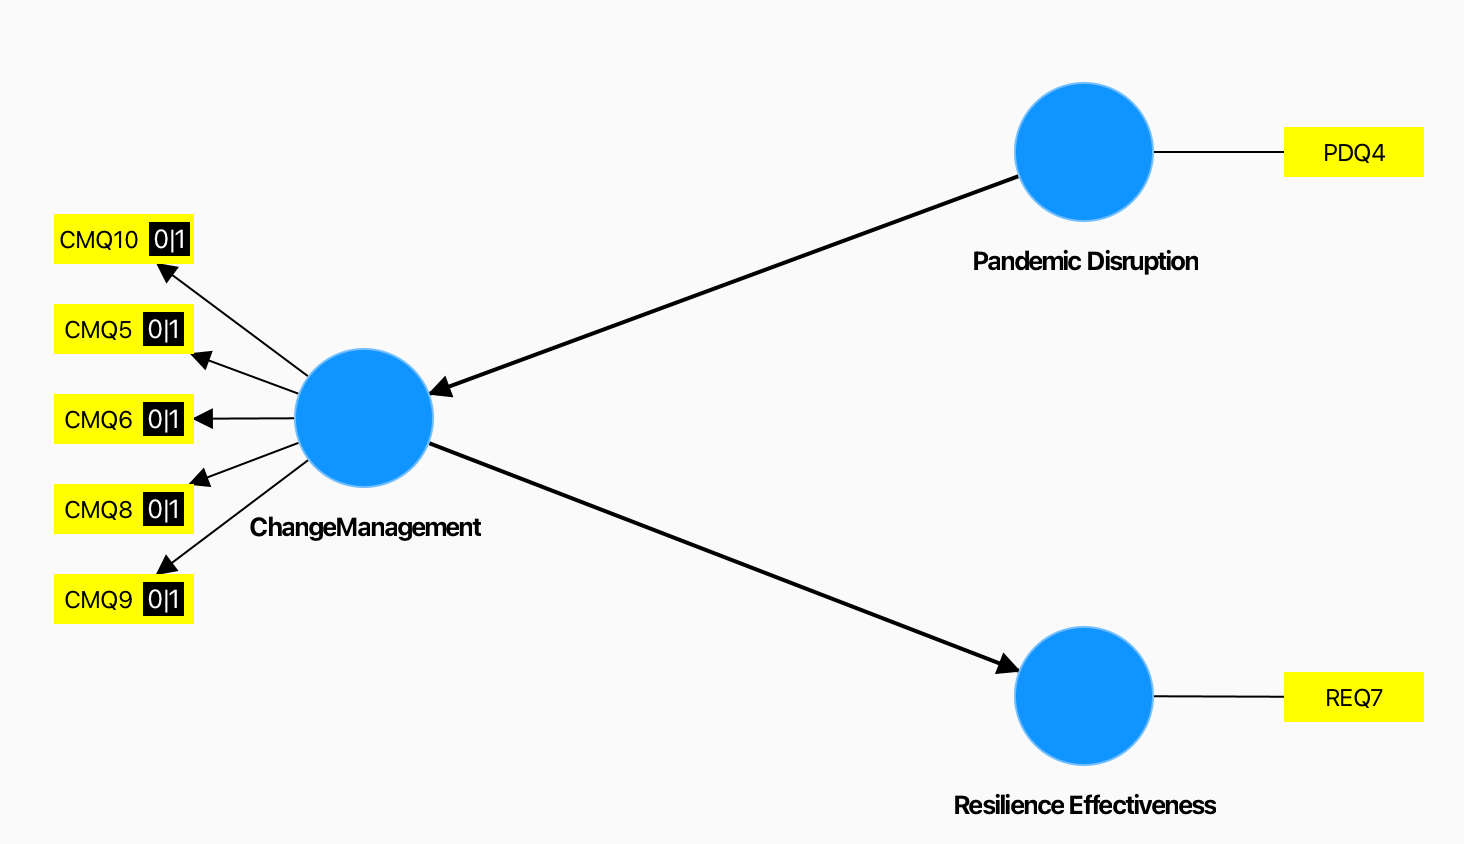
\includegraphics[width=1\textwidth]{figure/initial_model.png}
  \caption{Structural Model in SmartPLS showing the relationships between constructs. The model includes Pandemic Disruption (Q4), Change Management (Q5, Q6, Q8, Q9, 10), and Resilience Effectiveness (Q7). Arrows indicate hypothesized dependencies: Pandemic Disruption's impact on Change Management and Resilience Effectiveness, and Resilience Effectiveness's influence on Change Management. $[0|1]$ Adjacent to the question numbers indicate the binary nature of the questions. Other questions belong to the Likert Scale.}
  \label{fig:constructs}
\end{figure}


Using SmartPLS 4, we constructed a model (Figure \ref{fig:constructs}) to test our hypotheses. The structural model posits the following relationships:

\begin{enumerate}
    \item \textbf{Pandemic Disruption leads to Change Management (H1)}: This hypothesis suggests that higher levels of disruption due to the pandemic are positively associated with an increase in change management strategies. The arrow from Pandemic Disruption to Change Management in the diagram represents this hypothesis. The rationale is that significant disruptions necessitate strategic changes to adapt and mitigate the impact.

    \item \textbf{Resilience Effectiveness reduces the need for extensive Change Management (H2)}: This hypothesis proposes a negative relationship between the effectiveness of resilience strategies and the extent of change management. If a company’s existing resilience strategies are effective, it may not need to implement extensive changes. This is depicted by the arrow from Resilience Effectiveness to Change Management, indicating that effective resilience strategies can mitigate the need for further change.

    \item \textbf{Pandemic Disruption influences Resilience Effectiveness (H3)}: This hypothesis posits a positive relationship between the level of pandemic disruption and the perceived effectiveness of resilience strategies. Higher levels of disruption may prompt companies to evaluate and enhance their resilience strategies, thus leading to higher effectiveness. This relationship is shown by the arrow from Pandemic Disruption to Resilience Effectiveness in the diagram.

\end{enumerate}

Upon conducting the analysis using the SmartPLS tool for PLS-SEM, we can evaluate the validity of our hypothesized relationships among the constructs. By examining the path coefficients, significance levels (p-values), and the R² values for each endogenous construct, SmartPLS provides comprehensive insights into the strength and significance of the proposed causal paths. In our specific case, this involves assessing whether the hypothesized positive relationship between Pandemic Disruption and Change Management, the negative relationship between Resilience Effectiveness and Change Management, and the positive relationship between Pandemic Disruption and Resilience Effectiveness hold true. Additionally, the bootstrapping procedure available in SmartPLS allows us to obtain estimates of standard errors and confidence intervals, further solidifying our hypothesis testing. The evaluation of the model fit indices, such as the SRMR (Standardized Root Mean Square Residual), will help determine the overall adequacy of our model, enabling us to conclude whether the empirical data supports our theoretical propositions. Thus, the detailed results obtained from SmartPLS will enable us to confirm or refute our hypotheses with a considerable degree of statistical confidence. In configuring the SmartPLS software for our PLS-SEM analysis, several key settings were chosen to ensure interpretable results. We selected the Principal Component Analysis (PCA) weighting scheme, a common default choice, as it uses the first principal component of the block’s indicators as the composite score, providing a reliable and standard approach. To facilitate easier interpretation of path coefficients and enable comparisons across constructs, we opted for standardized results, which convert all variables to a common scale. For the initial weights, we adhered to the algorithm’s default settings. Regarding the handling of missing values, considering that only one response was partially missing, we utilized casewise deletion, provided it did not significantly reduce our sample size below acceptable limits for robust analysis. Lastly, we did not apply any additional weighting vectors, as none were necessary for our analysis.

\subsection{Results and Analysis of PLS-SEM}

\begin{figure}[h]
  \centering
  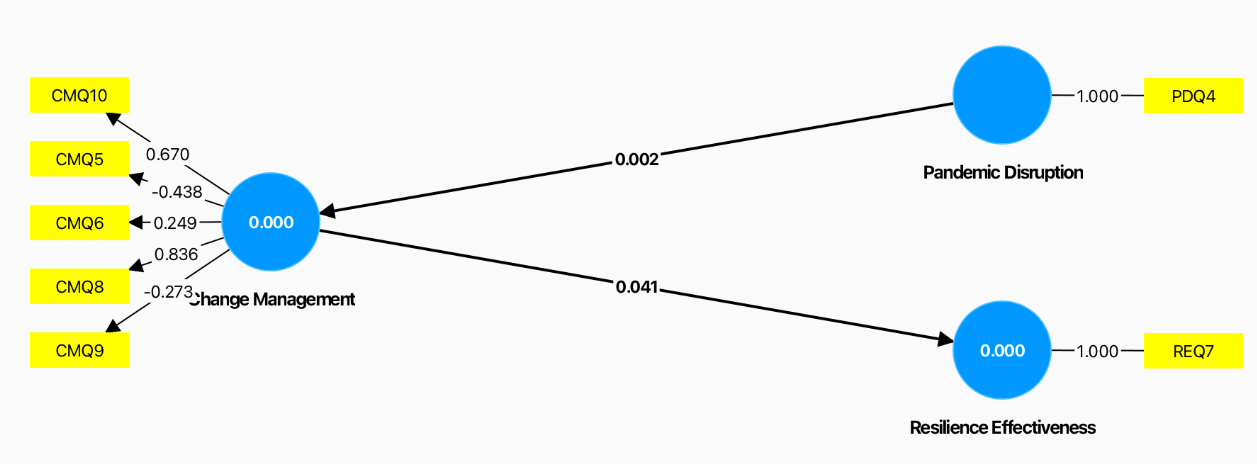
\includegraphics[width=1\textwidth]{figure/pls_sem_results_cropped.png}
  \caption{PLS-SEM Results showcasing path coefficients between constructs.}
  \label{fig:pls_sem_results}
\end{figure}

The results of our PLS-SEM analysis, depicted in Figure \ref{fig:pls_sem_results}, reveal the path coefficients among the constructs of Pandemic Disruption, Change Management, and Resilience Effectiveness. The path coefficient from Pandemic Disruption to Change Management is 0.002, suggesting a minimal positive influence of pandemic-induced disruptions on the extent of change management strategies implemented. This indicates that while pandemic disruptions might necessitate some strategic changes, the direct impact observed here is negligible. Conversely, the path coefficient from Resilience Effectiveness to Change Management is 0.041, implying a slight positive relationship. This suggests that as the effectiveness of resilience strategies increases, there is a marginal but positive impact on change management practices, indicating that companies with effective resilience strategies may still engage in proactive change management. The negative coefficients observed within the Change Management construct, such as -0.438 for CMQ5, -0.249 for CMQ6, and -0.273 for CMQ9, indicate that these specific aspects of change management may inversely relate to the overall construct. This could mean that certain change management practices, possibly those perceived as less effective or unnecessary, might detract from the overall strategic change efforts. The positive coefficients, such as 0.670 for CMQ10 and 0.836 for CMQ8, highlight the aspects that contribute positively to Change Management, signifying effective practices that enhance strategic adaptability. The significant values of 1.000 for PDQ4 and REQ7 indicate strong relationships of these specific questions with their respective constructs, emphasizing their reliability as indicators. Following the discussion on the path coefficients and their implications, we now turn our attention to additional metrics and validity assessments to provide further analysis of the model's performance.

\begin{figure}[h]
  \centering
  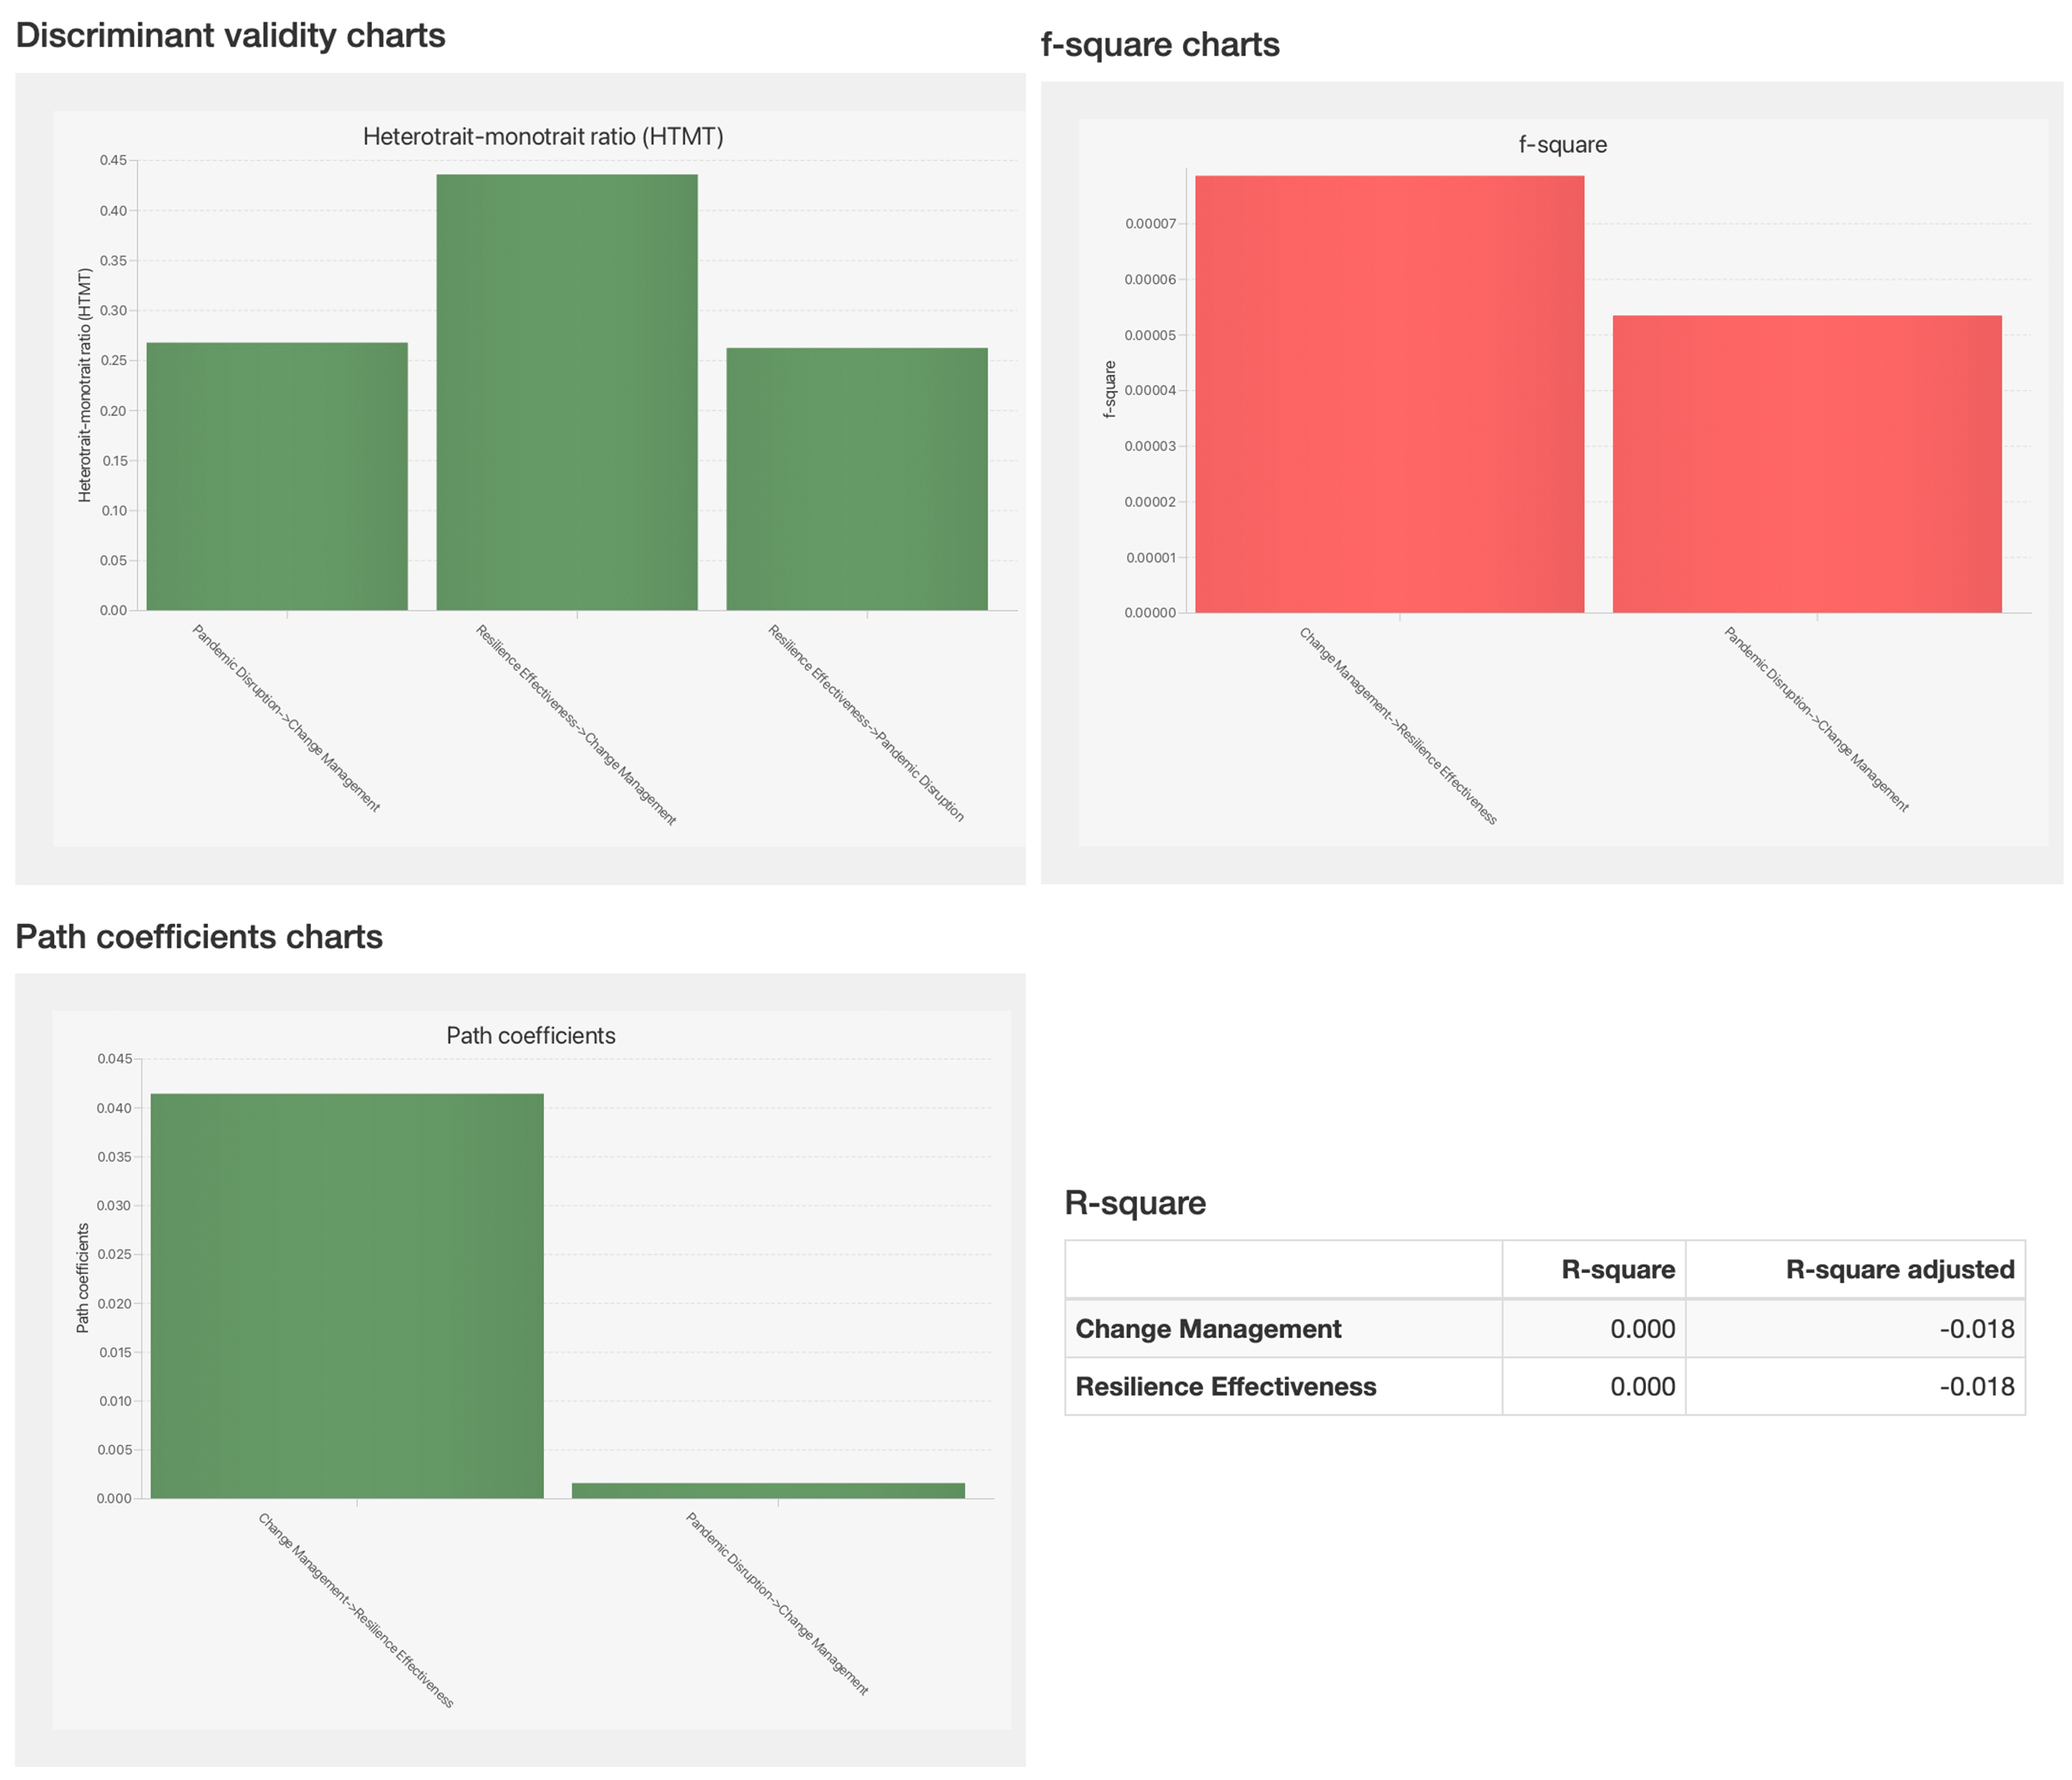
\includegraphics[width=1\textwidth]{figure/other_results.png}
  \caption{Other statistics from PLS-SEM analysis.}
  \label{fig:other_results}
\end{figure}

The results and analysis of PLS-SEM, as depicted in Figure \ref{fig:other_results}, offer further understanding of the relationships between the constructs of Pandemic Disruption, Change Management, and Resilience Effectiveness. The path coefficients chart confirms the previously discussed minimal impact, with the coefficient from Pandemic Disruption to Change Management being virtually zero (0.002), indicating a negligible direct effect. The slightly positive coefficient from Resilience Effectiveness to Change Management (0.041) suggests a weak but positive influence, implying that effective resilience strategies marginally contribute to change management efforts. The R-square values for both Change Management and Resilience Effectiveness are zero, indicating that the model does not explain any variance in these constructs, which may suggest either the lack of a strong relationship or limitations in the model's ability to capture the dynamics. The f-square values, though small, provide insight into the effect sizes, with Change Management to Resilience Effectiveness showing a slightly higher value compared to Pandemic Disruption to Change Management, indicating that resilience strategies have a somewhat more substantial influence on change management. The discriminant validity, assessed through the Heterotrait-Monotrait ratio (HTMT), indicates acceptable values below the threshold of 0.85, confirming that the constructs are distinct from each other. The SRMR (Standardized Root Mean Square Residual) values are 0.172 for the saturated model and 0.180 for the estimated model, both exceeding the recommended threshold of 0.08, suggesting a poor model fit and potential issues with the structural model specification. These results imply that while some relationships are weakly supported, the overall model does not adequately capture the variance and relationships between the constructs, indicating the need for model refinement or consideration of additional variables to better understand the dynamics at play.

Based on expert analysis and observation of our dataset, several factors have been identified that may explain why we were unable to establish strong correlations in our PLS-SEM analysis. Firstly, the lack of variability in the Change Management questions (CMQ5, CMQ6, CMQ8, CMQ9, CMQ10), where responses were predominantly '1' (Yes), significantly limits the statistical power of our analysis. The homogeneity in these responses means there is insufficient variation to explain the variance in dependent constructs, thereby hindering the detection of meaningful relationships. While the Pandemic Disruption variable (PDQ4) exhibited more variability, ranging from 0.8 to 5, its effectiveness in revealing correlations is compromised when paired with less variable indicators. Similarly, Resilience Effectiveness (REQ7) showed reasonable variability, ranging from 1.5 to 5, but the overall analysis suffers from the lack of diversity in binary responses. The binary nature and the high prevalence of a single response category diminish the ability of PLS-SEM to uncover underlying patterns, as significant paths are often established through variance explained by independent variables. The presence of potential ceiling effects, where binary indicators in the Change Management construct consistently hit the upper limit of their scale, further complicates the analysis by obscuring genuine relationships. This effect results in insufficient differentiation among responses, making it difficult to discern how changes in one variable relate to another. Lastly, the model configuration and theoretical considerations play a crucial role; our current model setup may not adequately capture the expected relationships if the theoretical assumptions are not perfectly aligned with the observed data. The predominance of 'yes' responses in the Change Management questions indicates that minor deviations might not statistically explain variations in Resilience Effectiveness, especially if the resilience question encompasses broader aspects of the pandemic's impact than anticipated. Consequently, while the results might indicate no correlation, it is also possible that due to the dataset's characteristics, existing correlations could not be established, highlighting the need for further refinement and consideration of additional variables.
















% \subsubsection{Purpose}
% Placeholder Text

% \subsubsection{Overview}
% Placeholder Text

% \subsection{Model Specification}
% Placeholder Text

% \subsubsection{Constructs and Measurement}
% Placeholder Text

% \subsubsection{Model Design}
% Placeholder Text

% \subsection{Evaluation of Measurement Model}
% Placeholder Text

% \subsubsection{Indicator Reality}
% Placeholder Text

% \subsubsection{Construct Reliability and Validity}
% \textbf{Internal Consistency Reliability}

% \textbf{Convergent Validity}

% \subsubsection{Discriminant Validity}

% \subsubsection{Summary}

% \subsection{Evaluation of Structural Model}

% \subsubsection{Path Analysis}
% \textbf{Path Coefficients}
% \textbf{Direct and Indirect Effects}

% \subsubsection{Model Fit}

% \subsubsection{R-Squared $(R^2)$ Values}

% \subsubsection{Effect Sizes $(f^2)$ Values}

% \subsection{Model Assessment and Validation}

% \subsubsection{Collinearity Statistics}

% \subsubsection{Robustness Checks}

% \subsection{Discussion of Findings}

% \subsubsection{Interpretation of Results}

% \subsubsection{Implications}

% \subsection{Limitations and Future Research Directions}

% \subsection{Conclusion}
% =====================PLS SEM SECTION




% RESULTS
\chapter{Results}

\section{Hypothesis Evaluation}
\todo[inline]{
    Note that this is only the results based on the interview, which is also currently partial. This section will be updated with the entire results for the research in the next submission.
}

\subsection{Evaluation of Hypothesis 1 and 2}

Based on the detailed analysis of the interview, we can determine that the evidence strongly supports Hypothesis 1, which asserts that suppliers of perishable goods faced significant disruptions in their supply chains due to the COVID-19 pandemic. The interview highlighted multiple challenges, such as supply shortages, transportation delays, and the need for rapid adjustments in inventory strategies. These challenges are consistent with the notion that the pandemic caused substantial disruptions across various supply chain components. For instance, the analysis accentuates that external events, such as the blockage of the Suez Canal, created severe transportation delays, leading to bottlenecks and increased complexity in demand forecasting. Such incidents illustrate the vulnerability of supply chains to sudden disruptions and emphasize the importance of flexibility in managing these challenges. The interview further revealed that managing transportation delays and shortages necessitated frequent recalibration of logistics and inventory management strategies, underscoring the reality of significant disruptions. Moreover, the presence of labor constraints and increased costs due to global health and safety regulations further validates Hypothesis 1. Although the interview did not directly delve into labor issues, it implied that disruptions in material availability and workforce management were critical challenges, contributing to higher operational costs and supply chain instability. Conversely, there is little to no evidence supporting Hypothesis 2, which suggests that suppliers of perishable goods did not experience substantial disruptions. The cumulative evidence points towards a broad range of disruptions, affecting both upstream and downstream supply chain activities.

Thus, the evaluation concludes that Hypothesis 1 is validated by the evidence presented in the interview, while Hypothesis 2 is contradicted by the same evidence. The interviewee's account of the supply chain challenges faced during the pandemic provides clear confirmation that the disruptions were significant, widespread, and required substantial adjustments to supply chain strategies and practices.

\subsection{Evaluation of Hypothesis 3 and 4}

In evaluating Hypothesis 3, which suggests that suppliers of perishable goods have implemented new strategies and procedures to enhance resilience and preparedness, the evidence from the interview provides strong support. The interview highlighted various immediate and long-term strategies that companies adopted in response to the pandemic, such as local warehousing, diversification of suppliers, and increased collaboration with both large and small suppliers. These strategies are indicative of a proactive approach aimed at strengthening supply chain resilience and preparing for future disruptions. Further evidence supporting Hypothesis 3 is seen in the long-term strategic changes implemented by companies, such as the adoption of technology for real-time data sharing and enhanced visibility across the supply chain. The creation of crisis management teams and the development of new supplier partnerships also demonstrate a commitment to improving preparedness for future crises. These changes reflect a strategic shift towards more resilient and flexible supply chains, which aligns with the hypothesis that companies have made significant efforts to enhance their resilience. Conversely, the evidence contradicts Hypothesis 4, which posits that suppliers have not implemented significant changes or strategies to enhance supply chain resilience. The findings show that companies have actively pursued various strategic responses to address the challenges posed by the pandemic. The use of technologies, establishment of crisis management teams, and the emphasis on continuous evaluation of supplier networks all point towards a deliberate effort to improve supply chain robustness.

In summary, the evidence from the interview strongly supports Hypothesis 3, demonstrating that suppliers have implemented various strategies to enhance resilience and preparedness. Meanwhile, Hypothesis 4 is contradicted by the findings, as companies have indeed made significant strategic changes to improve their supply chain resilience in anticipation of future disruptions.



% CONCLUSION
% \chapter{Timeplan}

Below is the tentative timeplan as proposed in the course guidelines:

% \usepackage{tabularx} % Include this line in the preamble of your document

\begin{table}[h]
\centering

\begin{tabularx}{\textwidth}{|l|X|X|}
\hline
\textbf{Date}         & \textbf{Milestone}                                          & \textbf{Deliverables}                                 \\ \hline
Feb 19, 2024          & Submit revised problem formulation, purpose, question, and first version of previous research and theory & Chapter on problem formulation, purpose, question, and previous research and theory \\ \hline
Mar 11, 2024          & Submit revised problem statement, purpose, question, and first version of method chapter                     & Revised chapters and first version of method chapter  \\ \hline
Apr 15, 2024          & Submit revised chapters and first version of analysis and final discussion chapter                           & Analysis chapter and final discussion chapter         \\ \hline
May 6, 2024           & Submit first version of entire thesis                                                                & Entire thesis                                         \\ \hline
May 13, 2024          & Supervisors notify course supervisor                                                     &                                                      \\ \hline
May 20, 2024          & Submission of final thesis version                                                      & Final thesis version                                  \\ \hline
May 22, 2024          & Contact examiner for opposition seminar                                                  &                                                      \\ \hline
\end{tabularx}

\caption{Thesis Timetable}
\label{tab:thesis_timetable}
\end{table}


\break
\section{Proposed Meeting Dates}

Below is the authors' proposed meeting dates with the thesis supervisor, subject to change after approval from the supervisor. 

\begin{table}[h]
\centering
\begin{tabular}{|l|p{10cm}|}
\hline
\textbf{Date}         & \textbf{Agenda}                                                                                               \\ \hline
Feb 13, 2024          & Review initial thesis structure and approach. Discuss problem formulation, purpose, and research questions. Guidance on conducting literature review. \\ \hline
Mar 7, 2024           & Review revised problem statement, purpose, and question. Feedback on initial research and theory. Discuss methodology chapter focusing on quantitative approach. \\ \hline
Apr 11, 2024          & Review revised problem formulation, purpose, question, and theory chapter. Discuss method chapter and analysis chapter. Initial discussion on final discussion chapter. \\ \hline
May 2, 2024           & Review first complete draft of thesis. Comprehensive feedback on all chapters. Discuss areas for refinement and preparation for submission. \\ \hline
May 14, 2024          & Review final version of thesis before submission. Final feedback and suggestions. Discussion on submission process and opposition seminar preparation. \\ \hline
\end{tabular}
\caption{Meeting Agendas}
\label{tab:meeting_agendas}
\end{table}

\chapter{Discussion}

The results of our study demonstrate significant alignment and, in some cases, divergence with the findings of previous research on supply chain resilience in the context of perishable goods during the COVID-19 pandemic. The integrated results from our PLS-SEM analysis and qualitative interviews provide insights into how suppliers were impacted by the pandemic and the strategies they adopted to enhance resilience. This discussion will compare our findings with the results reported in the studies cited above.

Our findings indicate that while there were substantial disruptions, including supply shortages, transportation delays, and increased operational costs, the suppliers did not significantly modify their management practices in response to these disruptions, as evidenced by the minimal direct impact of Pandemic Disruption on Change Management (0.002). This contrasts with the findings of \textcite{Sharma2022ImpactPerspective}, who emphasize that supplier visibility, facilitated by information sharing and supply chain traceability, significantly influences the adoption of sustainable practices and supply chain performance \parencite{Sharma2022ImpactPerspective}. The divergence can be explained by the focus of our study on the direct impact of disruption on management practices, whereas \textcite{Sharma2022ImpactPerspective}. examine how visibility affects sustainable practices indirectly. Our study highlights a more reactive approach by suppliers, primarily focusing on immediate crisis management rather than proactively enhancing sustainability. Nevertheless, it is important to note that the contrasting results obtained in our PLS-SEM analysis were also attributed to the lack of variance in our survey responses. 

With respect of another factor of Financial Performance and Preparedness, the negative impacts on financial performance due to the COVID-19 pandemic are also highlighted in our qualitative findings, where suppliers experienced increased operational costs and transportation delays. This aligns with the results of \textcite{Maharjan2023LogisticsPandemic}, who found that Japanese companies experienced both positive and negative impacts, with negative impacts predominantly affecting financial performance \parencite{Maharjan2023LogisticsPandemic}. However, our findings indicate that despite these financial setbacks, there was minimal change in management practices, whereas \textcite{Maharjan2023LogisticsPandemic} observed varying levels of preparedness and response strategies across different companies. This suggests that while the financial impact was universally felt, the extent of strategic changes and preparedness varied significantly across different contexts. 

Shifting focus to Strategies for Cold Supply Chain Resilience, both our study and the research by \textcite{Khan2023EnhancementCountry} identify the importance of logistics and inventory management in enhancing supply chain resilience. However, the authors specifically highlight "crisis simulation," "identification and securing of logistics," and "digitalization of cold supply chains" as critical strategies for maintaining the quality and resilience of cold supply chains \parencite{Khan2023EnhancementCountry}. Our findings support the adoption of these strategies, particularly the focus on logistics improvements, although "digitalization" was not identified as a key strategy, it is important to note that this was one of the strategies that was identified during the one-on-one interview discussed in the Section \ref{sec:intervew-analysis}. 

Additionally, in terms of Modeling Supply Chain Networks for Freshness and Cost Optimization, the emphasis on minimizing transmission risks and ensuring the freshness of goods in supply chains during the pandemic, as highlighted by \textcite{Asgharizadeh2023ModelingPandemic}, is consistent with our findings regarding the need for rapid adjustments to supply chain disruptions \parencite{Asgharizadeh2023ModelingPandemic}. Our study’s results, particularly from the qualitative interviews, align with the need for agile logistics strategies to maintain product freshness and manage operational costs. However, the modeling approach proposed by \textcite{Asgharizadeh2023ModelingPandemic}, involving optimization techniques and meta-heuristic algorithms, represents a more advanced and quantitative approach to addressing these challenges, which our study did not explore in depth.

When discussing the factors influencing supply chain resilience, our findings suggest that technology plays a supporting role in enhancing supply chain resilience through improved logistics and inventory management. This is partially aligned with the findings of \textcite{Ruamchart2023SupplyIndustry}, who identifies agility as the primary direct factor influencing supply chain resilience, with technology exerting an indirect effect through agility, flexibility, and collaboration \parencite{Ruamchart2023SupplyIndustry}. The indirect role of technology in our study is consistent with this view, suggesting that while technology is crucial, its primary impact may be in facilitating other resilience-enhancing factors, such as agility and flexibility. Furthermore, the concept of repurposing food supply chain management, as discussed by \textcite{Sangiumvibool-Howell2023RepurposingReview}, resonates with the strategic responses observed in our interviews, where suppliers diversified suppliers and improved logistics \parencite{Sangiumvibool-Howell2023RepurposingReview}. Both studies outline the need for adaptive strategies in managing food supply chains during the pandemic. However, our study focuses more on diversification and technological investments, while \textcite{Sangiumvibool-Howell2023RepurposingReview} emphasize re-purposing and localizing supply chains, suggesting a broader range of strategies in the literature.

In a different context of critical resilience factors, \textcite{Montanya2023ThePandemic} identify customer-oriented business awareness, proximity-based distribution models, and cooperative practices as critical resilience factors (albeit specifically in Agri-Food Supply Chains). These findings align with the strategic responses observed in our study, where diversification and improvements in logistics were key strategies adopted by suppliers. However, our study also emphasizes technological investments, which were not highlighted as prominently in \textcite{Montanya2023ThePandemic}'s review. This suggests a complementary view where both traditional (proximity-based and cooperative practices) and modern (technological) strategies are essential for building supply chain resilience.

The comparison of our findings with existing literature reveals a multidimentional approach to enhancing supply chain resilience during the COVID-19 pandemic. While there are areas of convergence, such as the emphasis on logistics improvements and the financial impacts of the pandemic, differences in the focus on technological investments and specific resilience strategies outline the diversity of approaches and contexts in supply chain management research. Our study contributes to this ongoing discourse by providing a nuanced understanding of how suppliers of perishable goods responded to the disruptions caused by the pandemic, complementing the existing body of knowledge with new insights on strategic adaptation and resilience-building efforts.

\section{Implications}

The results of this study have broader implications for both the theory and practice of supply chain management, particularly in the context of managing perishable goods during global disruptions. Beyond the immediate effects of the COVID-19 pandemic, the findings highlight the critical need for a paradigm shift in how supply chain resilience is approached. The minimal direct impact of pandemic disruptions on change management practices, as revealed by our PLS-SEM analysis, suggests that existing strategies and frameworks may be insufficient to address future crises. This calls for a more dynamic, adaptive approach that integrates flexibility, technological innovation, and robust contingency planning. Additionally, the qualitative insights from industry professionals emphasize the importance of fostering agile and responsive supply chains that can rapidly adjust to disruptions. This suggests the necessity for supply chain managers and policymakers to rethink traditional risk management strategies, moving towards a more holistic, system-wide perspective that considers both the micro and macro-level challenges in a rapidly changing global landscape. Furthermore, these results encourage further research into new models and frameworks that better capture the complexity and uncertainty of modern supply chains, ultimately contributing to a more resilient and sustainable supply chain ecosystem in the face of future global disruptions.

\chapter{Conclusion}

While this thesis aimed to investigate the impact of the COVID-19 pandemic on the supply chains of perishable goods and to explore the strategies adopted by suppliers to enhance resilience during the pandemic and in anticipation of future disruptions, this study has several limitations.

 

 \section{Limitations}
In this section we discuss the challenges and obstacles we faced while performing the research. The work undertaken could be a part of a larger study and multifaceted approach to the segment dividing the perishable goods into it's subcategories such as vegetables, fruits, meat and dairy, etc.

 \subsection{Anonymity and Lack of Data Granularity}

 One of the key limitations of our study was the decision not to record any identifying information about the participants, in order to comply with ethical standards and data protection regulations. While this ensured the anonymity and confidentiality of the respondents, it also introduced a significant limitation: we were unable to link responses back to specific individuals, countries, companies, or job positions. This lack of granularity in the data meant that while we knew which countries, companies, and positions were targeted, we could not directly associate specific responses with these variables. Consequently, our analysis could not account for potential differences in responses based on these factors, which may have provided additional insights into the impact of the pandemic on different segments of the supply chain. 

 

 \subsection{Survey Design Constraints}

 Another limitation was related to the survey design itself. Initially, we developed a more extensive set of questions, which we sent to a small group of known contacts for feedback. The feedback indicated that the survey was too lengthy, particularly given that participation was voluntary and no incentives were offered. Respondents expressed reluctance to complete a long survey, which led us to significantly shorten the questionnaire. The final survey consisted of only 10 questions, with 7 designed for quantitative analysis and 1 for qualitative analysis. This reduction in the number of questions limited the depth of the data we could collect, particularly in terms of more focused or detailed inquiries that might have provided richer insights. 

The trade-off, however, was an increased likelihood of participation, which was crucial given the challenges of obtaining responses without offering incentives. While we took significant steps to ensure the ethical treatment of participants and to protect their privacy, these measures also introduced limitations in the scope and depth of our analysis. The constraints imposed by the need for anonymity, the voluntary nature of the survey, and the decision to limit the number of questions all impacted the breadth and specificity of the data collected. These limitations are acknowledged and should be carefully considered when interpreting the findings of this study.

 

 \subsection{Model Fit in PLS-SEM Analysis}
 The PLS-SEM model employed exhibited poor fit, indicating that the chosen constructs may not have fully captured the complexity of the relationships between pandemic disruptions, resilience strategies, and change management. Future research should consider additional variables that may better explain these relationships.

 

 \subsection{Sector Focus}
 The study's scope was limited to suppliers of perishable goods. While this provided valuable insights specific to this sector, the generalizability of the findings to other sectors remains limited.

 

 \subsection{Incorporating Additional Variables}
 Future studies should explore other factors influencing change management and resilience, such as organizational culture, government policies, and external market conditions. These could provide a more holistic view of the factors shaping supply chain resilience during crises.

 \section{Future Research Directions}

This study opens several avenues for future research:

\subsection{Sector-Specific Strategies}
While the findings provide a broad view of resilience strategies, more focused studies are required to explore how these strategies can be tailored to meet the unique demands and challenges of different industries. Each sector presents its own regulatory frameworks, operational dynamics, and risks, and future research should aim to develop sector-specific adaptations of resilience strategies.

\subsection{Scalability of Integrated Supply Chain Models}
While strategies such as the integration of online and offline retail channels (e.g., "buy online, pick up in-store" or BOPS) have been explored in some models, there is a need for deeper research into the scalability and practical implementation of such models across various supply chain networks. Investigating sector-specific challenges, particularly for perishable goods, could yield valuable insights into how such models enhance resilience.

\subsection{Longitudinal Studies on Strategy Effectiveness}
Future research should consider conducting longitudinal studies to track the effectiveness of the resilience strategies adopted during the pandemic over time. Understanding the long-term outcomes of these strategies could help establish best practices and identify the conditions under which these strategies succeed or need modification.

\subsection{Role of Emerging Technologies}
As digital tools and technologies play an increasing role in supply chain management, future studies should explore how technologies such as artificial intelligence, blockchain, and the Internet of Things (IoT) can be integrated into supply chain resilience strategies. A deeper exploration of their scalability, sector-specific applications, and impact on resilience would contribute significantly to the field.

 Results of our research contributes to the understanding of how suppliers of perishable goods were impacted by the COVID-19 pandemic and how they responded to enhance their supply chain resilience. The study highlights that while significant disruptions occurred, suppliers adopted a range of short-term and long-term strategies to mitigate these impacts. Diversified supplier bases, innovation, and operational continuity were among the key strategies employed, indicating a proactive approach to building supply chain resilience.

However, the limitations imposed by the need for anonymity, the shortened survey design, and the poor fit of the PLS-SEM model suggest that further research is needed to expand on these findings. More granular data collection, sector-specific studies, and the exploration of digital tools in supply chain management can provide deeper insights and improve the preparedness of supply chains for future disruptions. Future research should aim to address these gaps and help businesses enhance their operational resilience in an increasingly unpredictable global environment.

 

% REFERENCES / BIBLIOGRAPHY
\cleardoublepage
\addcontentsline{toc}{chapter}{Bibliography}
% \input{include/backmatter/References}
\printbibliography

% APPENDICES
\cleardoublepage
\appendix
\setcounter{page}{1}
\pagenumbering{Roman}	% Capitalized roman numbering starting from I (one)

\chapter{Appendix 1 - Survey Questionnaire}
\label{appendix:survey}

\noindent Please complete the following questions regarding your company's supply chain management:

\begin{enumerate}[label=\textbf{Q\arabic*:},leftmargin=*]
    \item What type of perishable goods does your company supply? (Select all that apply)\\
    \textit{Perishable goods include any food which is likely to decay faster and has limited shelf life if it's not refrigerated.}
    \begin{enumerate}[label=\arabic*., leftmargin=2em]
        \item Vegetables
        \item Dairy products
        \item Meat and poultry
        \item Seafood
        \item Other: (Please write down)
    \end{enumerate}
    
    \item What is the turnover of your company?\\
    \textit{Annual turnover in terms of USD Million.}
    \begin{enumerate}[label=\arabic*., leftmargin=2em]
        \item Less than 0.5 million USD
        \item Between 0.5 to 2 million USD
        \item Greater than 2 million USD
    \end{enumerate}
    
    \item What is the size of your company?\\
    \textit{In terms of manpower employed.}
    \begin{enumerate}[label=\arabic*., leftmargin=2em]
        \item Small enterprise employing between 10 to 49 persons
        \item Medium enterprise employing between 50 to 249 persons
        \item Large enterprise employing more than 250 persons
    \end{enumerate}
    
    \item To what extent did the COVID-19 pandemic disrupt your supply chain for perishable goods?\\
    \textit{Scale: 1 - Not at all, 5 - Very significantly.}
    
    \item Did your company implement any changes to its supply management strategies during the pandemic?
    \begin{enumerate}[label=\arabic*., leftmargin=2em]
        \item Yes
        \item No
    \end{enumerate}
    
    \item Did you diversify your supplier base for perishable goods in response to the pandemic?
    \begin{enumerate}[label=\arabic*., leftmargin=2em]
        \item Yes
        \item No
    \end{enumerate}
    
    \item How effective were your existing resilience strategies (e.g., inventory management, supplier diversification) in mitigating the impact of the pandemic?
    \textit{Scale: 1 - Not effective at all, 5 - Extremely effective.}
    
    \item Did your company create backup plans for critical parts of the supply chain to ensure continuity during disruptions?
    \begin{enumerate}[label=\arabic*., leftmargin=2em]
        \item Yes
        \item No
    \end{enumerate}
    
    \item Did you adjust your demand forecasting methods to better respond to market changes during the pandemic?
    \begin{enumerate}[label=\arabic*., leftmargin=2em]
        \item Yes
        \item No
    \end{enumerate}
    
    \item Does your company have a formal pandemic preparedness plan in place for future events?
    \begin{enumerate}[label=\arabic*., leftmargin=2em]
        \item Yes
        \item No
    \end{enumerate}
    
    \item We would really appreciate it if you can add some insights based on your personal experience of handling supply chain issues during the pandemic.
    \begin{itemize}[leftmargin=2em]
        \item -- Subjective answer
    \end{itemize}
\end{enumerate}



\chapter{Appendix 2 - Interview Questionnaire}
\label{appendix:interview}

\begin{enumerate}[leftmargin=*, label=\textbf{\arabic*.}]
    \item Can you tell me any specific vulnerabilities within supply chain?
    \begin{itemize}[label=$\rightarrow$]
        \item \textit{Follow-up:} Have you experienced health-related problems in the food industry?
    \end{itemize}

    \item Can you provide an example of a health-related problem in the food industry?

    \item How is it possible to have complete end-to-end visibility in the supply chain?
    \begin{itemize}[label=$\rightarrow$]
        \item \textit{Follow-up:} What are the challenges in achieving this?
    \end{itemize}

    \item What strategies can we use to avoid overreliance on single sources to mitigate risk?

    \item How flexible and adaptable is our supply chain in responding to changes in demand or supply?
    \begin{itemize}[label=$\rightarrow$]
        \item \textit{Follow-up:} Can you share an experience related to this from the food industry?
    \end{itemize}

    \item What is the optimal inventory strategy that balances cost efficiency and other factors?
    \begin{itemize}[label=$\rightarrow$]
        \item \textit{Follow-up:} How does this apply globally, particularly in temperature-controlled transport?
    \end{itemize}

    \item How can we enhance collaboration with suppliers and partners to improve transparency, trust, and joint risk management?
    \begin{itemize}[label=$\rightarrow$]
        \item \textit{Follow-up:} What kind of collaboration would be effective during a pandemic?
    \end{itemize}

    \item Do you think AI, IoT, and other technologies are helpful in the supply chain?
    \begin{itemize}[label=$\rightarrow$]
        \item \textit{Follow-up:} How can these technologies solve tracking and traceability challenges?
    \end{itemize}

    \item How do we ensure compliance with global regulations and commitment to sustainability?
    \begin{itemize}[label=$\rightarrow$]
        \item \textit{Follow-up:} What are the specific strategies for reducing waste and ensuring proper use of resources?
    \end{itemize}

    \item Do we have any comprehensive crisis management plans that include supply chain disruption?
    \begin{itemize}[label=$\rightarrow$]
        \item \textit{Follow-up:} How was this handled during the COVID-19 pandemic?
    \end{itemize}

    \item What strategies are important for rapid recovery from supply chain disruptions?
    \begin{itemize}[label=$\rightarrow$]
        \item \textit{Follow-up:} Can you provide any specific examples of recovery strategies?
    \end{itemize}

    \item What were the most significant challenges faced with perishable goods during COVID-19?

    \item Do you have any main concerns regarding the potential impact of future pandemics on perishable goods?

    \item What are the most important measures the perishable goods industry can take to improve resilience for future pandemics?

\end{enumerate}


\newpage

%Header Last Page
\vtop{
    \null\vspace{-47.5mm}
    \centerline{\textcolor{thesisHeaderColor}{\rule{1.28\textwidth}{28mm}}}
    \null\vspace{-9mm}
    \centerline{\textcolor{headerBrown}{\rule{1.28\textwidth}{4pt}}}
    \vspace{187mm}
    \if\ThesisType M
    \centerline{
\includegraphics[width=0.2\pdfpagewidth]{figure/auxiliary/logo_circle.png}}
    \fi
    \if\ThesisType B
    \centerline{
\includegraphics[width=0.2\pdfpagewidth]{figure/auxiliary/logo_circle.png}}
    \fi
    \vspace{-220mm}
}

\addtolength{\voffset}{2cm}
\renewcommand{\familydefault}{\sfdefault} \normalfont % Set cover page font
\pagestyle{empty}
\vspace*{-4.3cm}
\noindent
\textcolor{white}{\footnotesize \textbf{\dept}\\
\textbf{\university} \\
\address \\
\href{\site}{\textcolor{white}{\site}}}



\end{document}